\clearpage

% --------------------------------------------------------------------------------------------

\section {$\bar{\nu}_e$ appearance analysis}
\label{sec:nuebarapp}

The significance to $\bar{\nu}_e$ appearance was given as a p-value.
The marginalisation method is used and all the Super-K samples are analyzed simultaneously.
The oscillation parameters priors used for the marginalisation are shown in \cref{tab:osc_params_joint_priors}.
Two different test statistics were used: rate-only and rate+shape

\subsection{Rate-only analysis method}
\label{sec:nuebarapp_rateonly}

The total number of observed events ($N_{obs}$), without using any information from the 
reconstructed energy shape, was used to quote the rate-only p-value. 
In order to simultaneously analyze 
all the Super-K samples a different procedure with respect to the one used in 2015 analysis
\cite{OurRun56AntiNueBarAppearanceAnalysis3Flavour}, 
where toys were performed by using the posterior distributions of the Run 1-4 Bayesian analysis,
has been adopted. 
For a single fit the following procedure was used:

\begin{itemize}
\item $N_{marg}$ toy experiments were performed taking into account only systematic uncertainties, but not the statistical fluctuations
\item For each toy the likelihood $\lambda_{marg}$ was calculated using eq.~\ref{eq:likemarg} and including only the samples which are not 
	affected by $\bar{\nu}_e$ appearance: neutrino mode muon-like, neutrino mode electron-like and antineutrino mode muon-like (called ``other samples")
\item Using the likelihood as a probability distribution function, 
	$\lambda_{marg}$ was then applied as a weight to the total number of observed events (of the toy) in the antineutrino mode electron-like sample
\item The procedure is repeated for all the $N_{marg}$ toy experiments. 
\end{itemize}

$N_{marg}$ is the number of marginalization toy experiments, which are needed to marginalise the systematic parameters and 
must be distinguished from the toy experiments that are used as fake-data sets in order to perform the p-value calculation.
Indeed the latter toys are performed by applying both systematic and statistical uncertainties.

It is worth to note that reweighting the number of events with the likelihood computed with the ``other samples", 
is mathematically the same as performing a likelihood ratio fit of the ``other samples", taking the posterior distribution of the systematic parameters 
and using it to extract the systematic parameters in a toy experiment.

The advantage of this method is that correlations between all the samples are taken correctly into account.
In the 2015 analysis the oscillation parameters were extracted from the Run 1-4 posterior distributions of the Bayesian analysis,
but the flux, cross section and detector systematic parameters priors were unaffected by the Run 1-4 data fit.
The difference between the two methods is negligible since the antineutrino mode $e$-like sample has a much lower statistic 
compared to the other samples, however this new method allows to take all the correlations into account correctly and 
to perform the analysis in one single step without making two different fits, one to obtain the oscillation parameters priors and the other to fit the antineutrino mode $e$-like data.




\subsection{Rate+shape analysis method}
\label{sec:nuebarapp_rateshape}

The rate+shape analysis method is similar to what is described in \ref{sec:cl}, with 
the difference that the test statistic is defined as:
 
\begin{align}
\Delta \chi^2 = \chi^2(\beta=0) - \chi^2(\beta=1)
\end{align}

where $\beta$ is the discrete parameter of interest that can take only 0 or 1 values.
This test statistic simply compare the oscillation with the non-oscillation hypothesis
but does not use the best-fit $\chi^2$ value.
More details are given in sec.\ref{sec:pvalue_nuebarapp}.
The method is analogue to what was used in \cite{OurRun56AntiNueBarAppearanceAnalysis3Flavour},
with the only difference that now all the Super-K samples are fitted simultaneously
and not only the antineutrino mode $e$-like one.

%--------------------------------------------------------------------------------------------------------------------                                                                                    

\subsection {P-value}
\label{sec:pvalue_nuebarapp}

% Describe the p-values used for the analysis

There are different test statistics which can be used to quote a p-value,
as described in 
~\cite{slides_davide_pvalue_asg} % ASG talk
.
As proposed by the OA group, for this $\bar{\nu}_e$ appearance search two different p-values are quoted.
In order to quote the significance given null $\bar{\nu}_e$ appearance, the parameter of interest is set to $\beta=0$
and $n=10k$ toys are performed.
The systematic parameters are randomized taking into account the correlations as described in \cref{sec:systematics:inputs}.
Then the $E_{reco}$ Vs $\theta$ distribution is fluctuated with Poisson. 
Then the following p-values are calculated:
\begin{itemize}

\item p-value with rate-only analysis: the number of events is used as test statistics, without using the shape information of the reconstructed energy 
	distribution. The distribution $f(N_{SK})$ of the total number of Super-K events in a toy ($N_{SK}$) is obtained from the performed toys. 
	Then the number of events is measured from the data set ($N_{SK}^{obs}$) and
	the 1-sided (right tail) p-value is computed in the following way: 	
	
	\begin{equation}
	\text{p-value (right tail)} = \int_{N_{SK}^{obs}}^{+\infty} f(N_{SK}) d N_{SK}  = 
		\frac{ \sum_{ itoy=1 }^{n} w(N_{SK} \geq N_{SK}^{obs} )^{itoy} }{ n }
	\end{equation}
	\label{eq:pvalue_rateonly}
	
	where $w(N_{SK} \geq N_{SK}^{obs})$ is 1 if $N_{SK} \geq N_{SK}^{obs}$ otherwise 0.
	The distribution $f(N_{tot}^{toy})$ is expected to be discrete since it follows the Poisson distribution.
			 
	In an analogous way the left tail 1-sided p-value is computed as following:
		
	\begin{equation}
	\text{p-value (left tail)} = \int^{N_{SK}^{obs}}_{-\infty} f(N_{SK}) d N_{SK}  = 
		\frac{ \sum_{ itoy=1 }^{n} w(N_{SK} \leq N_{SK}^{obs} )^{itoy} }{ n }
	\end{equation}
	\label{eq:pvalue_rateonly}
		 
\item p-value with rate+shape analysis: the shape information of the reconstructed energy distribution is used.
	In this case the test statistic is used to compare the case of $\beta=0$ with $\beta=1$:
	
	\begin{equation}
	\Delta \chi^2 = \chi^2(\beta=0) - \chi^2(\beta=1)
	\end{equation}
	\label{eq:deltachisq_rateshape}

	where $\chi^2(\beta=0)$ and $\chi^2(\beta=1)$ are computed using \cref{eq:loglikemarg}.
	It is worth to note that the parameter $\beta$ is not fitted but fixed either to 0 or 1.
	The 1-sided p-value (right tail) is calculated as:

	\begin{equation}
	\text{p-value (right tail)} = \int_{\Delta \chi^2_{obs}}^{+\infty} f(\Delta \chi^2) d \Delta \chi^2  = 
		\frac{ \sum_{ itoy=1 }^{n} w(\Delta \chi^2 \geq \Delta \chi^2_{obs} )^{itoy} }{ n }
	\end{equation}
	\label{eq:pvalue_rateonly}
	
	where $w(\Delta \chi^2  \geq \Delta \chi^2 _{obs})$ is 1 if $\Delta \chi^2  \geq \Delta \chi^2 _{obs}$ otherwise 0.

	The 1-sided p-value (left tail) is calculated as:

	\begin{equation}
	\text{p-value (left tail)} = \int^{\Delta \chi^2_{obs}}_{-\infty} f(\Delta \chi^2) d \Delta \chi^2  = 
		\frac{ \sum_{ itoy=1 }^{n} w(\Delta \chi^2 \leq \Delta \chi^2_{obs} )^{itoy} }{ n }
	\end{equation}
	\label{eq:pvalue_rateonly}
	
\end{itemize}

The p-value will be calculated on the left or right tail depending on the position of the observed test statistic
in the expected distribution. For example, if the observed test statistic is on the left tail of the expected distribution of the
test statistic, a 1-sided p-value is computed on the left tail. Otherwise a 1-sided p-value on the right tail is computed. 

%--------------------------------------------------------------------------------------------------------------------                                                                                    

\clearpage


\section {Sensitivity to $\bar{\nu}_e$ appearance}
\label{sec:sensitivity_nuebarapp}

As discussed within the OA group, 
since there are not fitted parameters in the analysis, the validation can 
be done by comparing the rate-only with rate+shape p-values and 
checking if the corresponding distributions are reasonable.
Of course the final validation is given if all the oscillation analyses agree.
This is done by performing a sensitivity study to $\bar{\nu}_e$ appearance
both with the Asimov dataset, which consists of the most probable dataset
that is the nominal expected $E_{reco}$ Vs $\theta$ distribution ~\cite{Asimov},
as well as for toy distributions, given a value of $\beta$.

The significance to $\bar{\nu}_e$ appearance is quoted 
%for 
%\TotalPotRHC1RePOT
%both \FakePotLow and 
%\FakePotHigh POT
using the procedure described in \cref{sec:pvalue_nuebarapp}.
In order to quote the significance to $\bar{\nu}_e$ appearance a 1-sided p-value (right tail) is computed.
In addition an mean p-value is also computed by performing \NumToysLarge toys.

%--------------------------------------------------------------------------------------------------------------------

\subsection {Asimov rate-only p-value}
\label{subsec:rateonly}

The expected Asimov rate-only p-value is given by the Asimov dataset A for $\beta=1$. 
The corresponding oscillation parameters are shown in \cref{tab:osc_params_joint_asimov},
The distribution of the number of superK events used as test statistic is shown in \cref{fig:pvalue_rateonly}. 
The expected number of events is
%3.718 for \FakePotLow POT 
%and 4.183 for  \FakePotHigh POT. 
%The quoted p-value is 
%and 0.113 for \FakePotLow POT.
%and 0.0538 for \FakePotHigh POT.
3.218 and the quoted p-value is XXX.
In \cref{tab:summary_sensi_rateonly} the rate-only p-value is shown
for different numbers of observed events.

\begin{figure}
\center
%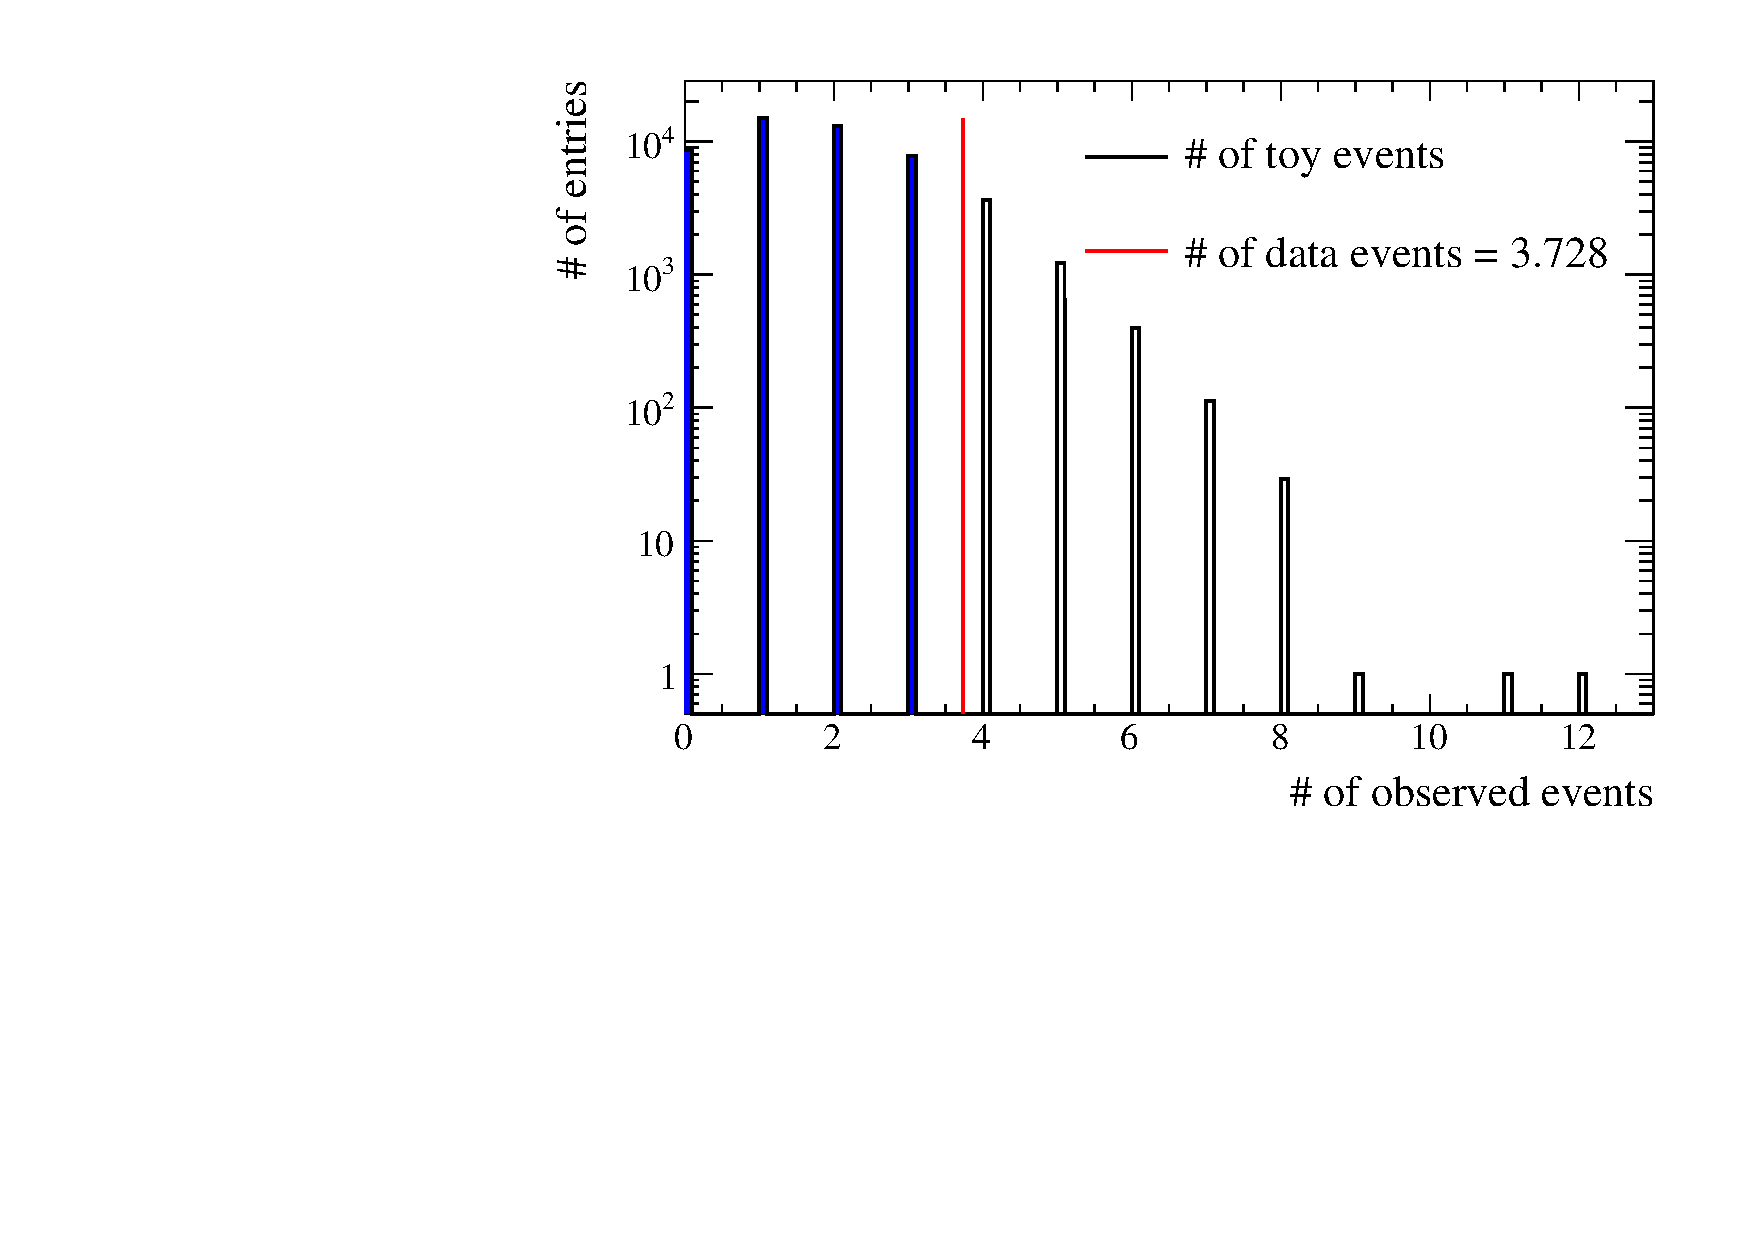
\includegraphics[width=0.9\textwidth]{./nuebar_plots/pvalue_median/pvalue_rate_4p0108E20POT_50ktoys.pdf}
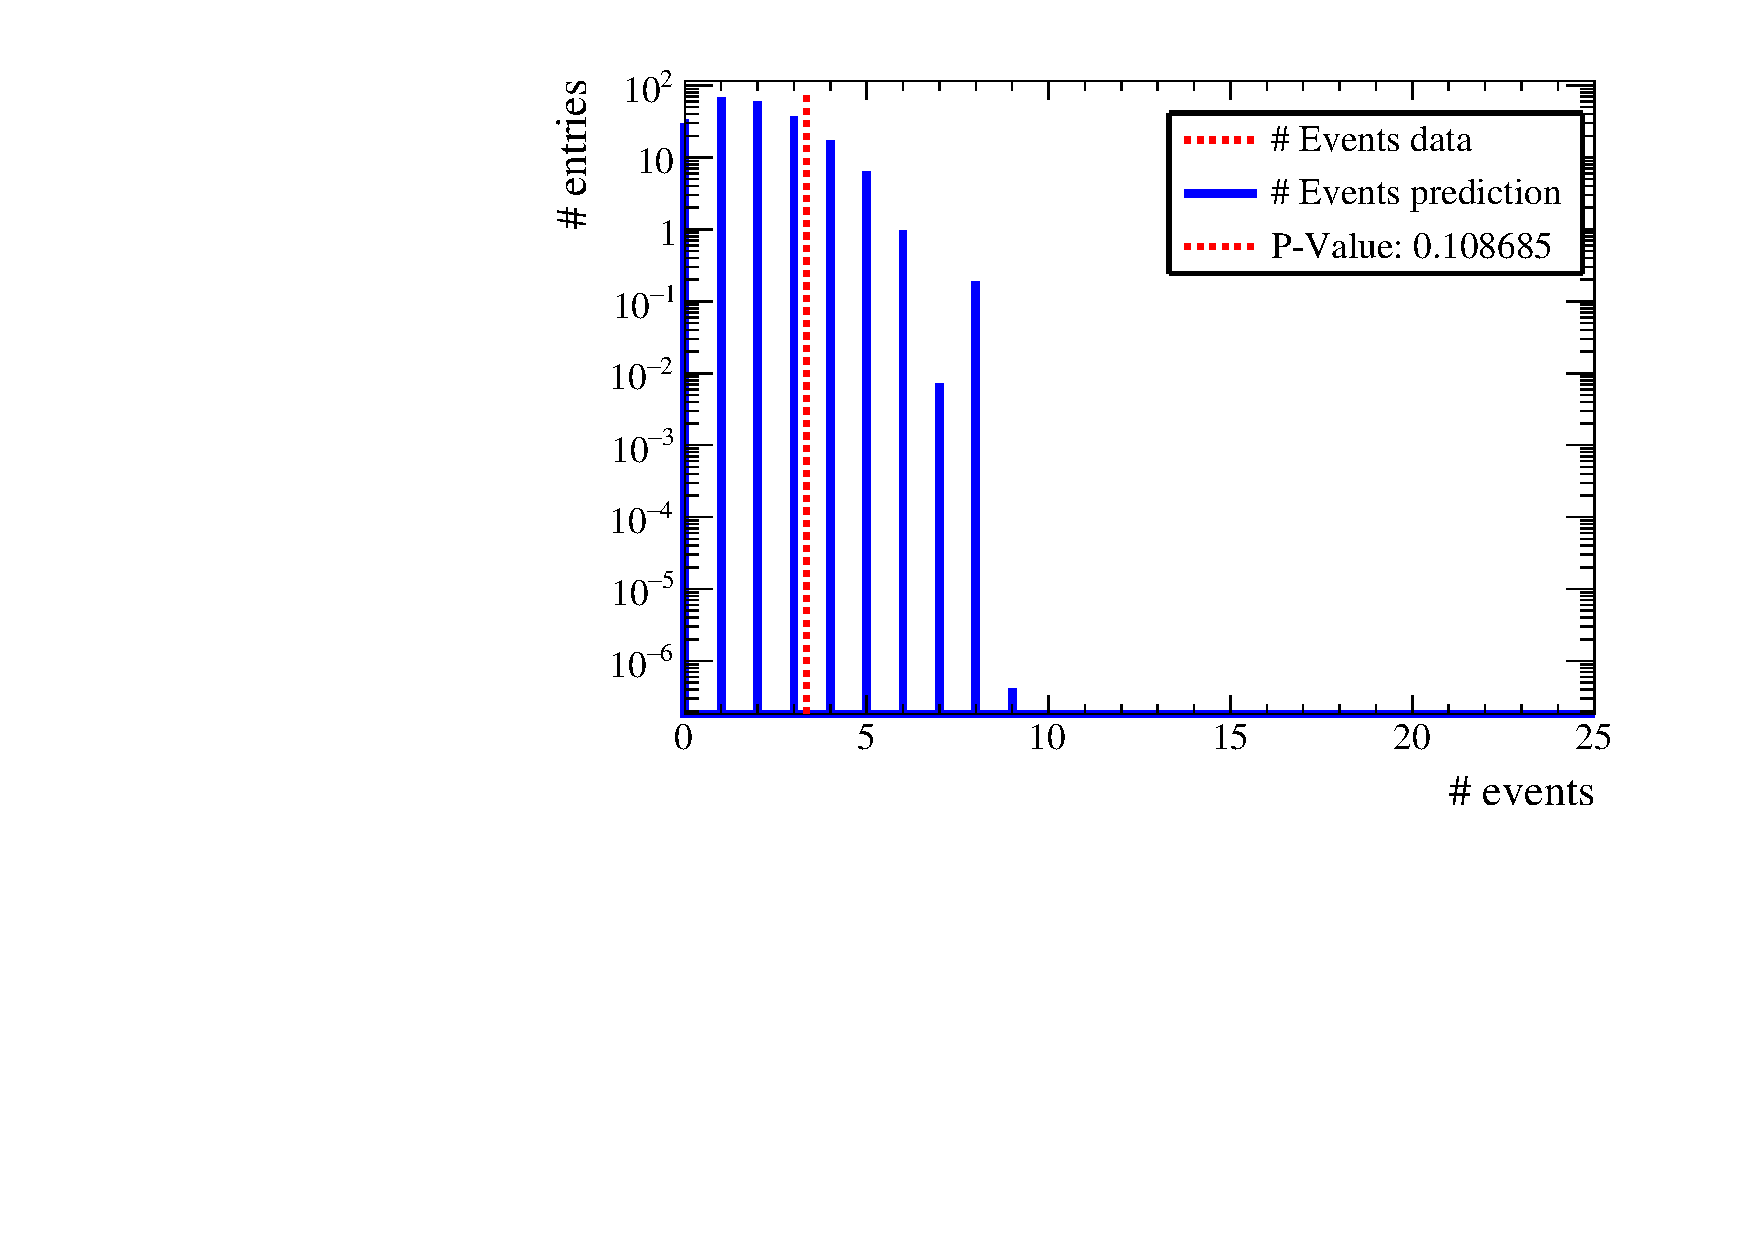
\includegraphics[width=0.6\textwidth]{./joint_plots/nuebar/rateonly/Asimov_beta1.pdf}
\caption {
%{\huge TO UPDATE} 
The distribution of the total number of events from each of the \NumToysLarge toy experiments. 
The red line corresponds to the total number of events given by the Asimov dataset. 
%The study is done with \TotalPotNuBar POT.
%\FakePotLow POT (left) and \FakePotHigh (right).
}
\label{fig:pvalue_rateonly}
\end{figure}

%--------------------------------------------------------------------------------------------------------------------




\subsection {Asimov rate+shape p-value}
\label{subsec:rateshape_median}


The expected distribution of $\Delta \chi^2$ for all the \NumToysLarge 
toy experiments
is shown in \cref{fig:pvalue_rateshape} for 
Run 1-6 statistic.
The $\Delta \chi^2$ from the Asimov dataset is 1.416.
The Asimov expected p-value is 0.0858 for the Run 1-6 statistic.

\begin{figure}
\center
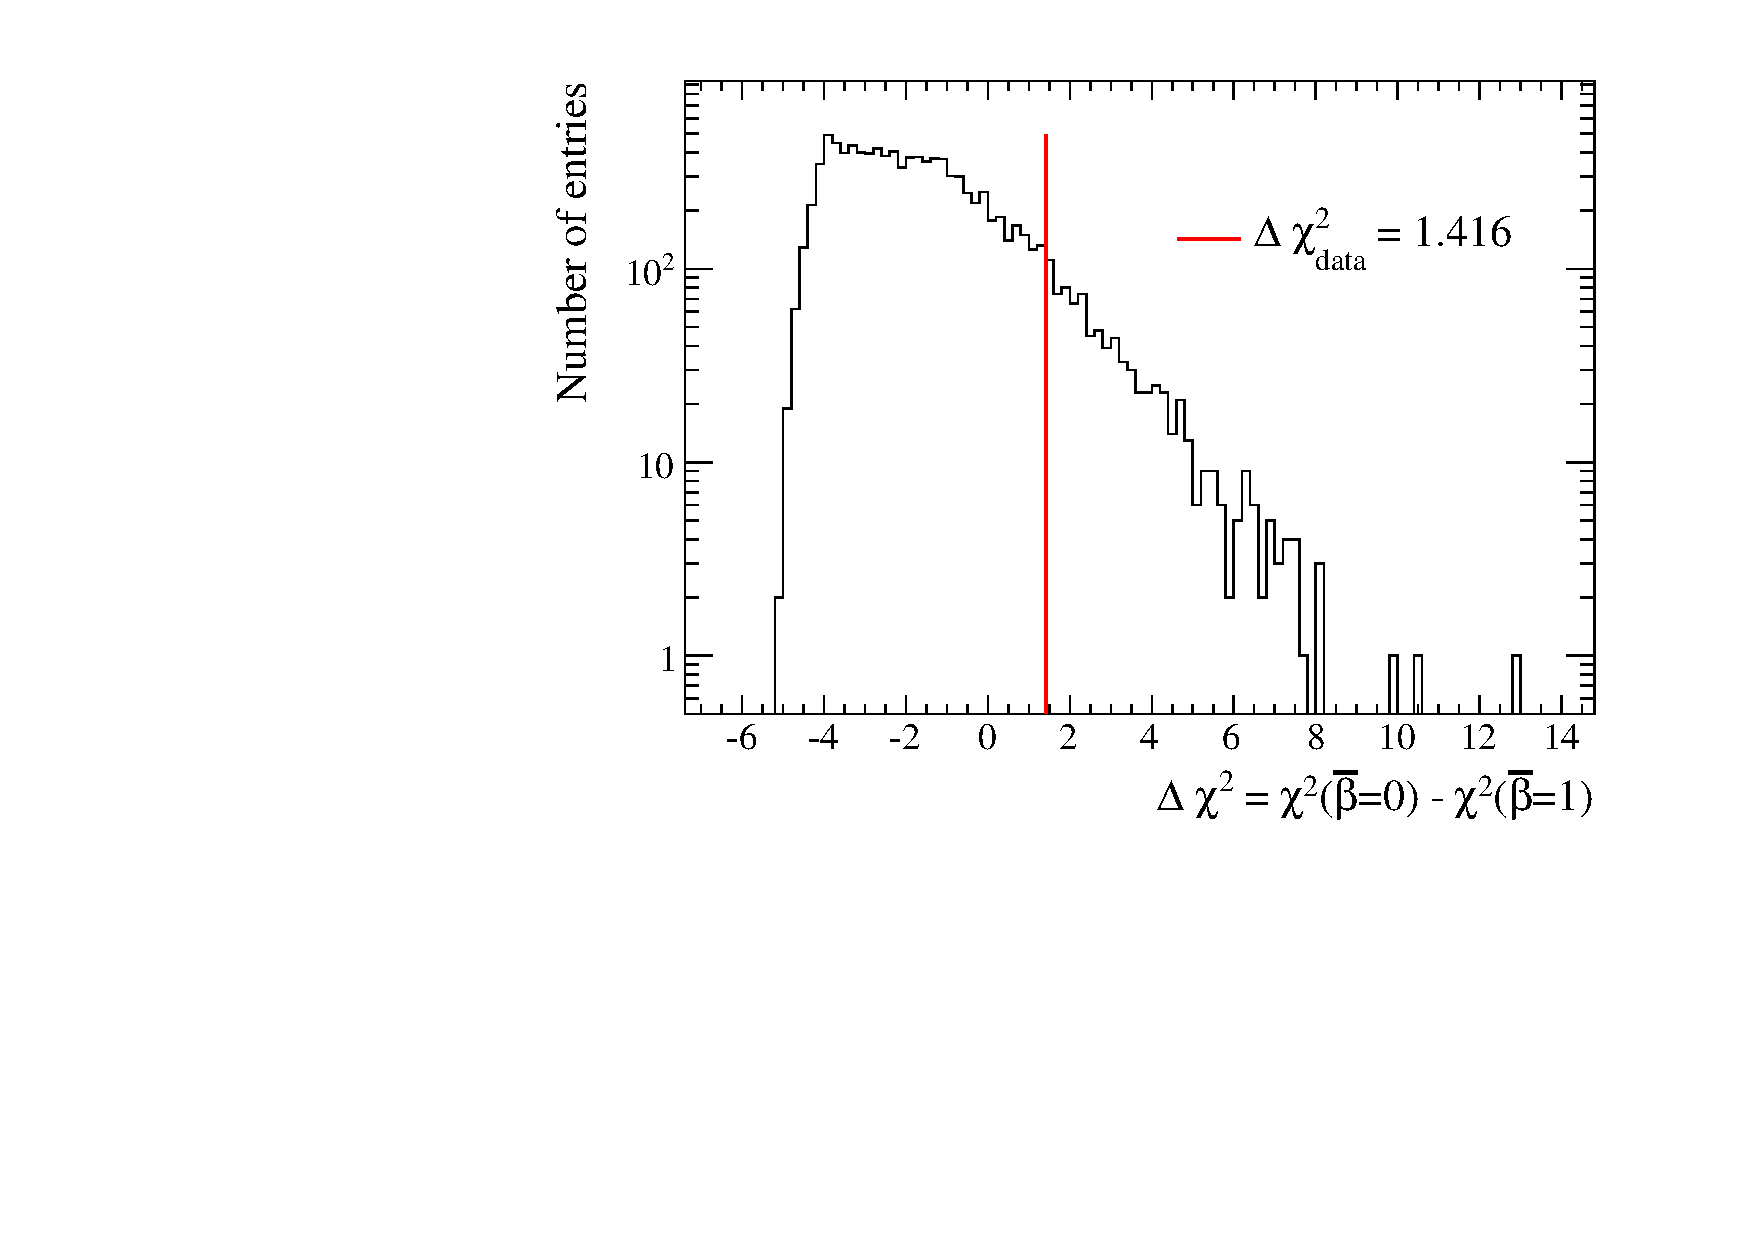
\includegraphics[width=0.48\linewidth]{./joint_plots/nuebar/rateshape/deltachisq_betabar_run16_10ktoys.pdf}
\caption {
Distribution of the $\Delta \chi^2$ for each of the \NumToysLarge 
toy experiments. 
The red line corresponds to $\Delta \chi^2$ obtained from the fit of the Asimov dataset A. 
The study is done with 
Run 1-6 statistic.
}
\label{fig:pvalue_rateshape}
\end{figure}

The p-value for the Asimov dataset as a function of $\beta$ or the total number of events is shown for 
Run 1-6 statistic
in \cref{fig:pvalue_Vs_beta_lowpot} and \cref{fig:pvalue_Vs_nevents_lowpot}. 

\begin{figure}
\center
%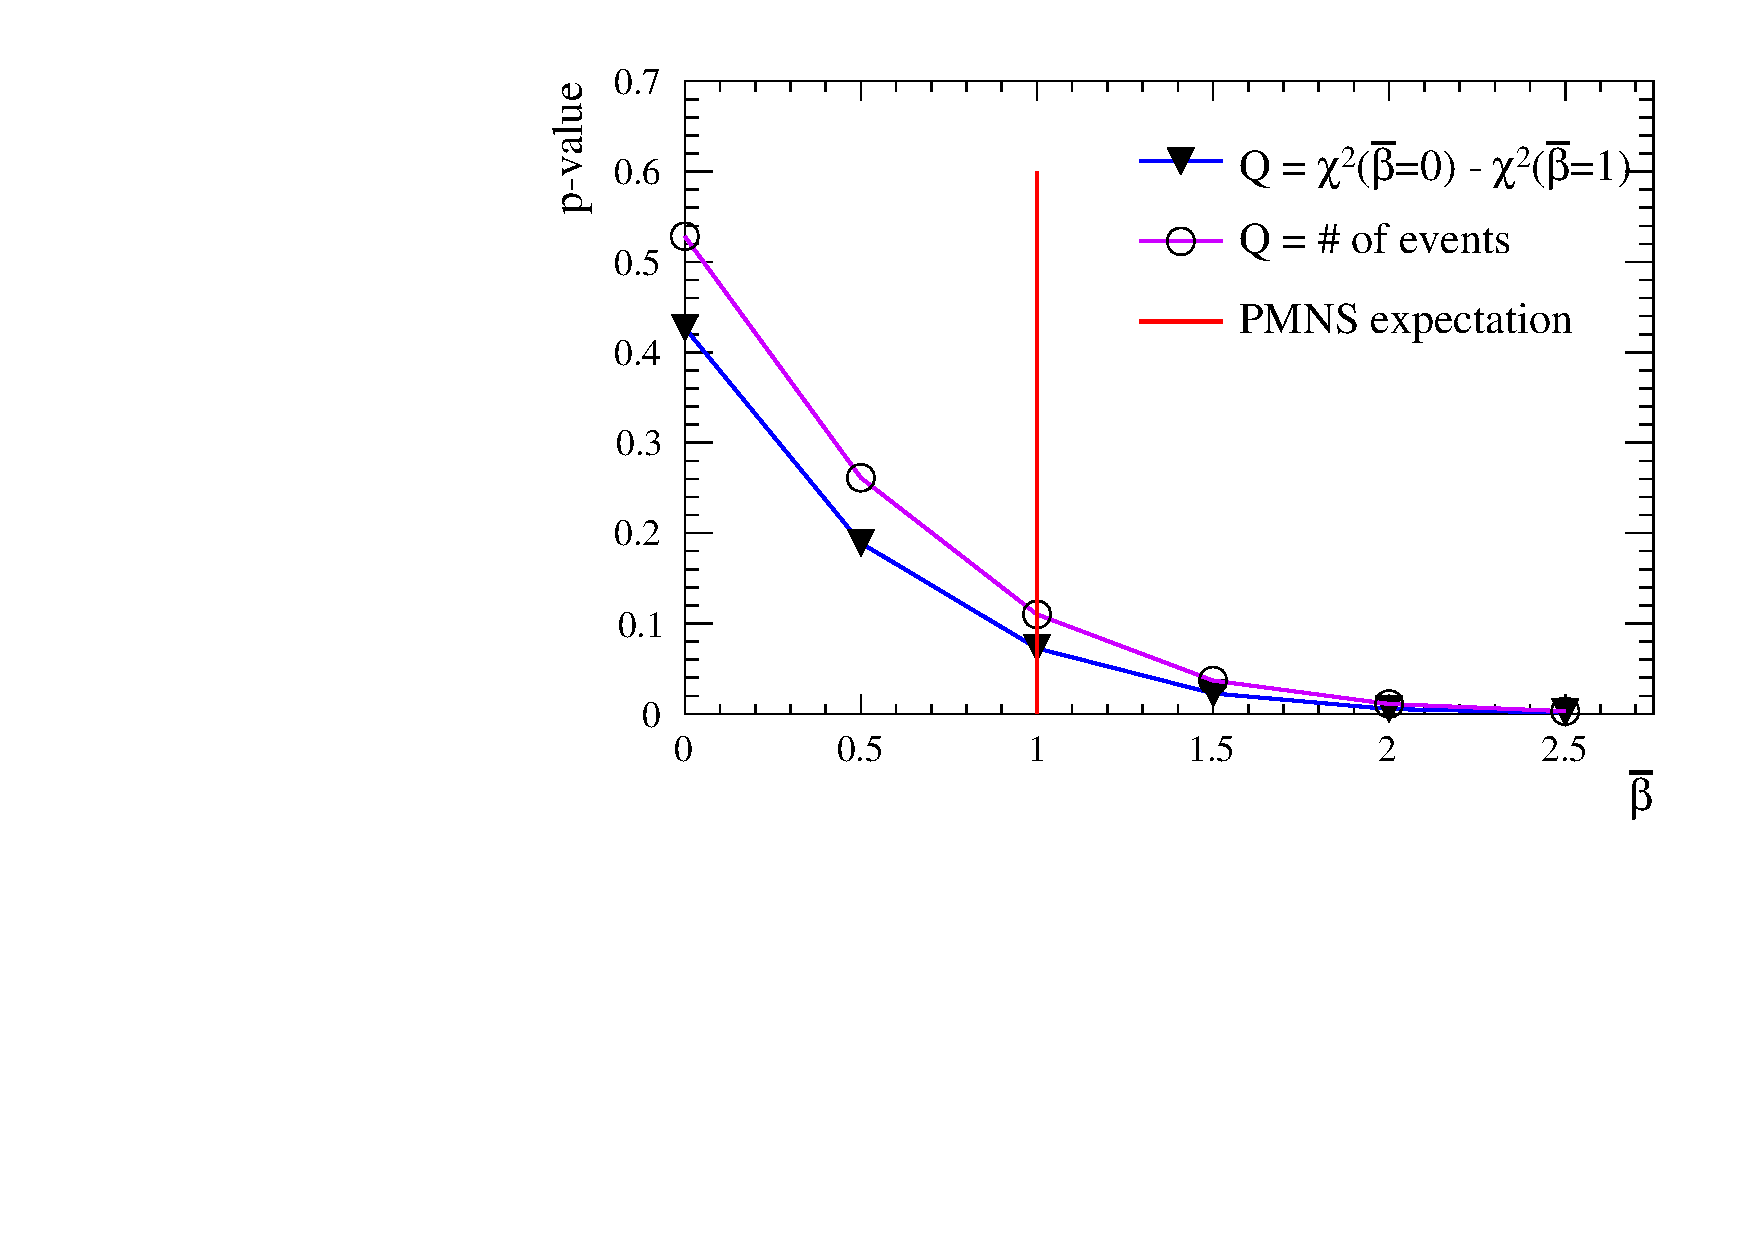
\includegraphics[width=0.48\linewidth]{./nuebar_plots/sensitivity/pvalue_Vs_beta_4p0108E20POT.pdf}
%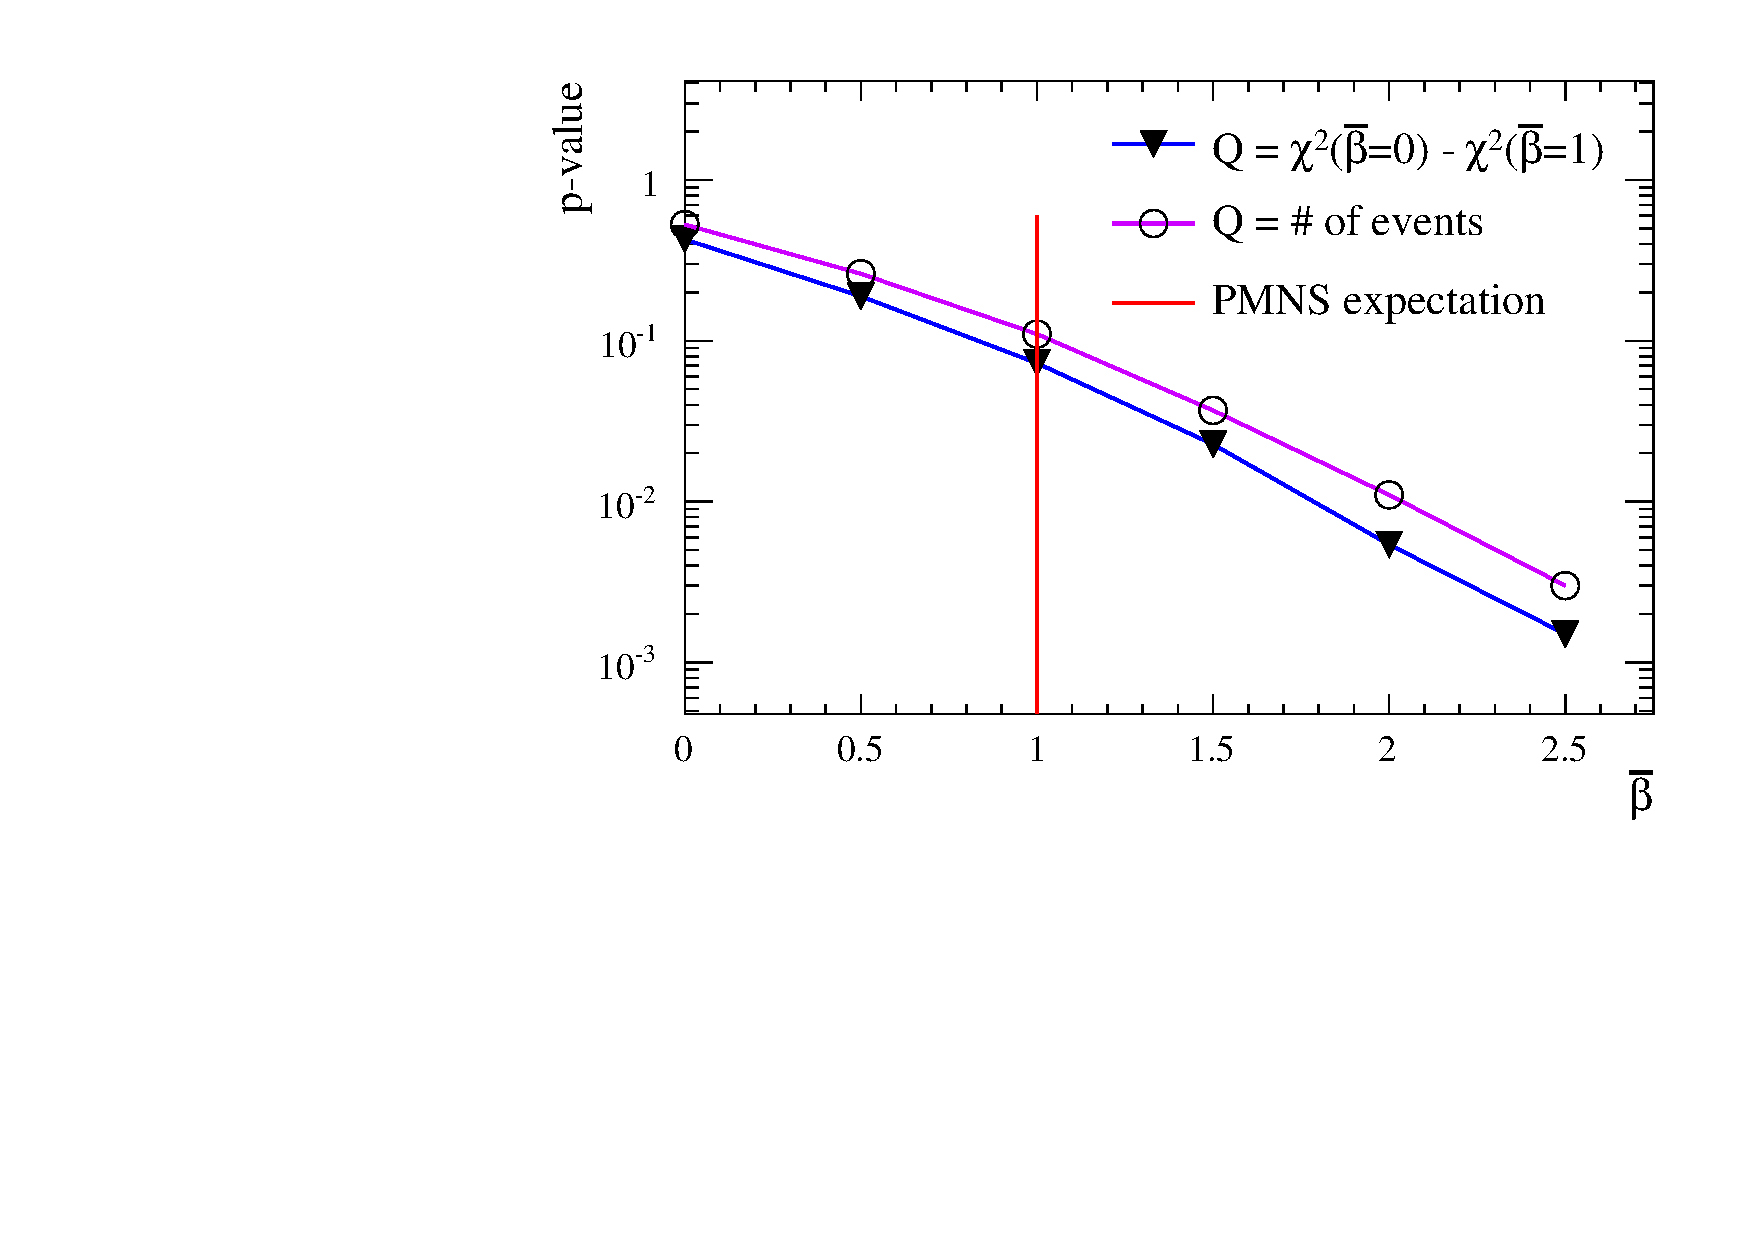
\includegraphics[width=0.48\linewidth]{./nuebar_plots/sensitivity/pvalue_Vs_beta_4p0108E20POT_log.pdf}
\begin{subfigure}[b]{0.49\textwidth}
\center
%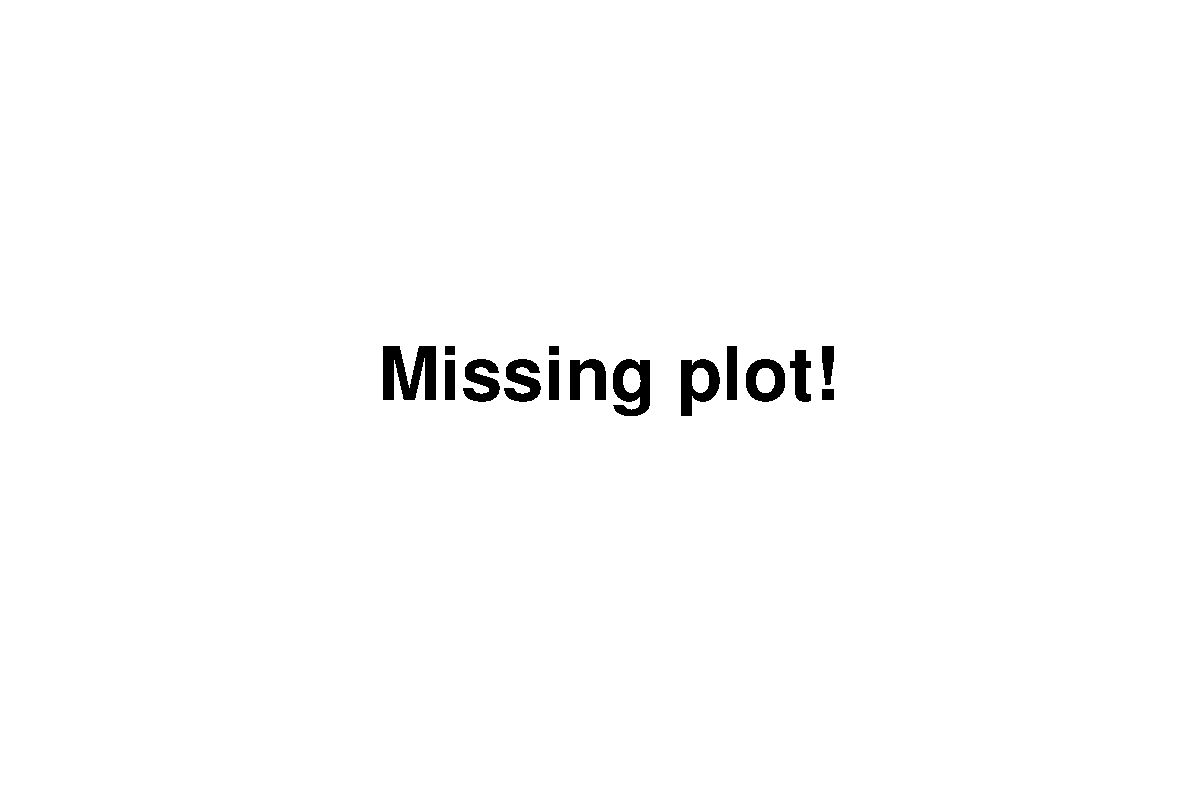
\includegraphics[width=0.9\textwidth]{./images/missing_plot-eps-converted-to.pdf}
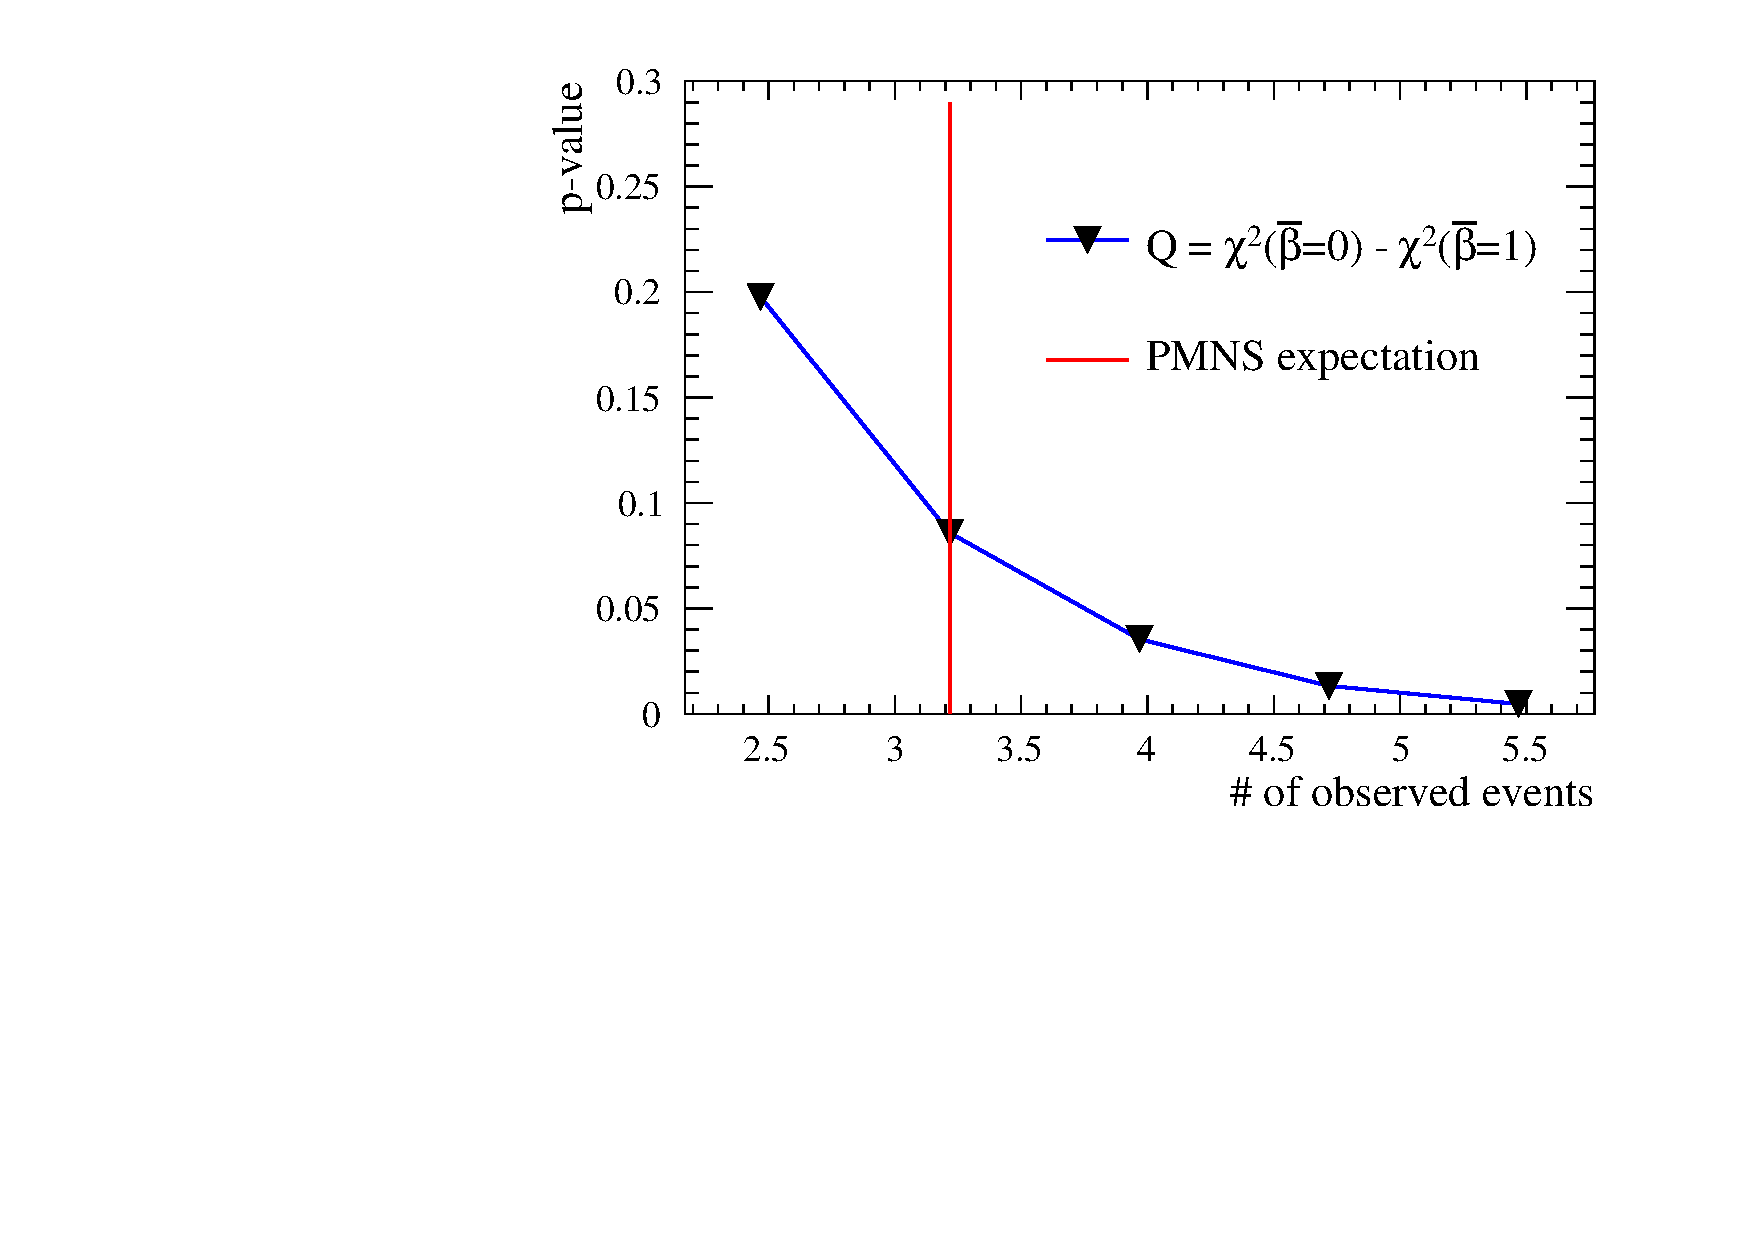
\includegraphics[width=0.9\linewidth]{./joint_plots/nuebar/rateshape/pvalue_Vs_nevt_ratepshape.pdf} 
\caption{Something}
\end{subfigure}
\begin{subfigure}[b]{0.49\textwidth}
\center
%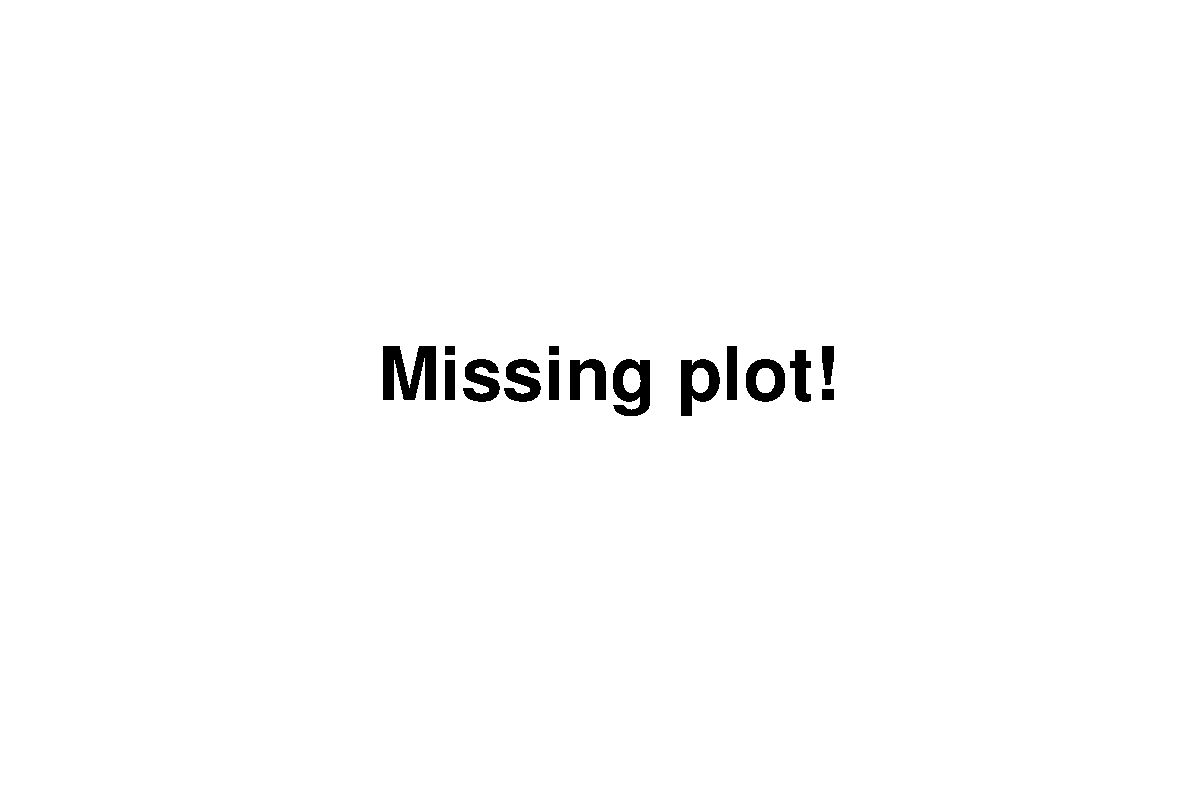
\includegraphics[width=0.9\textwidth]{./images/missing_plot-eps-converted-to.pdf}
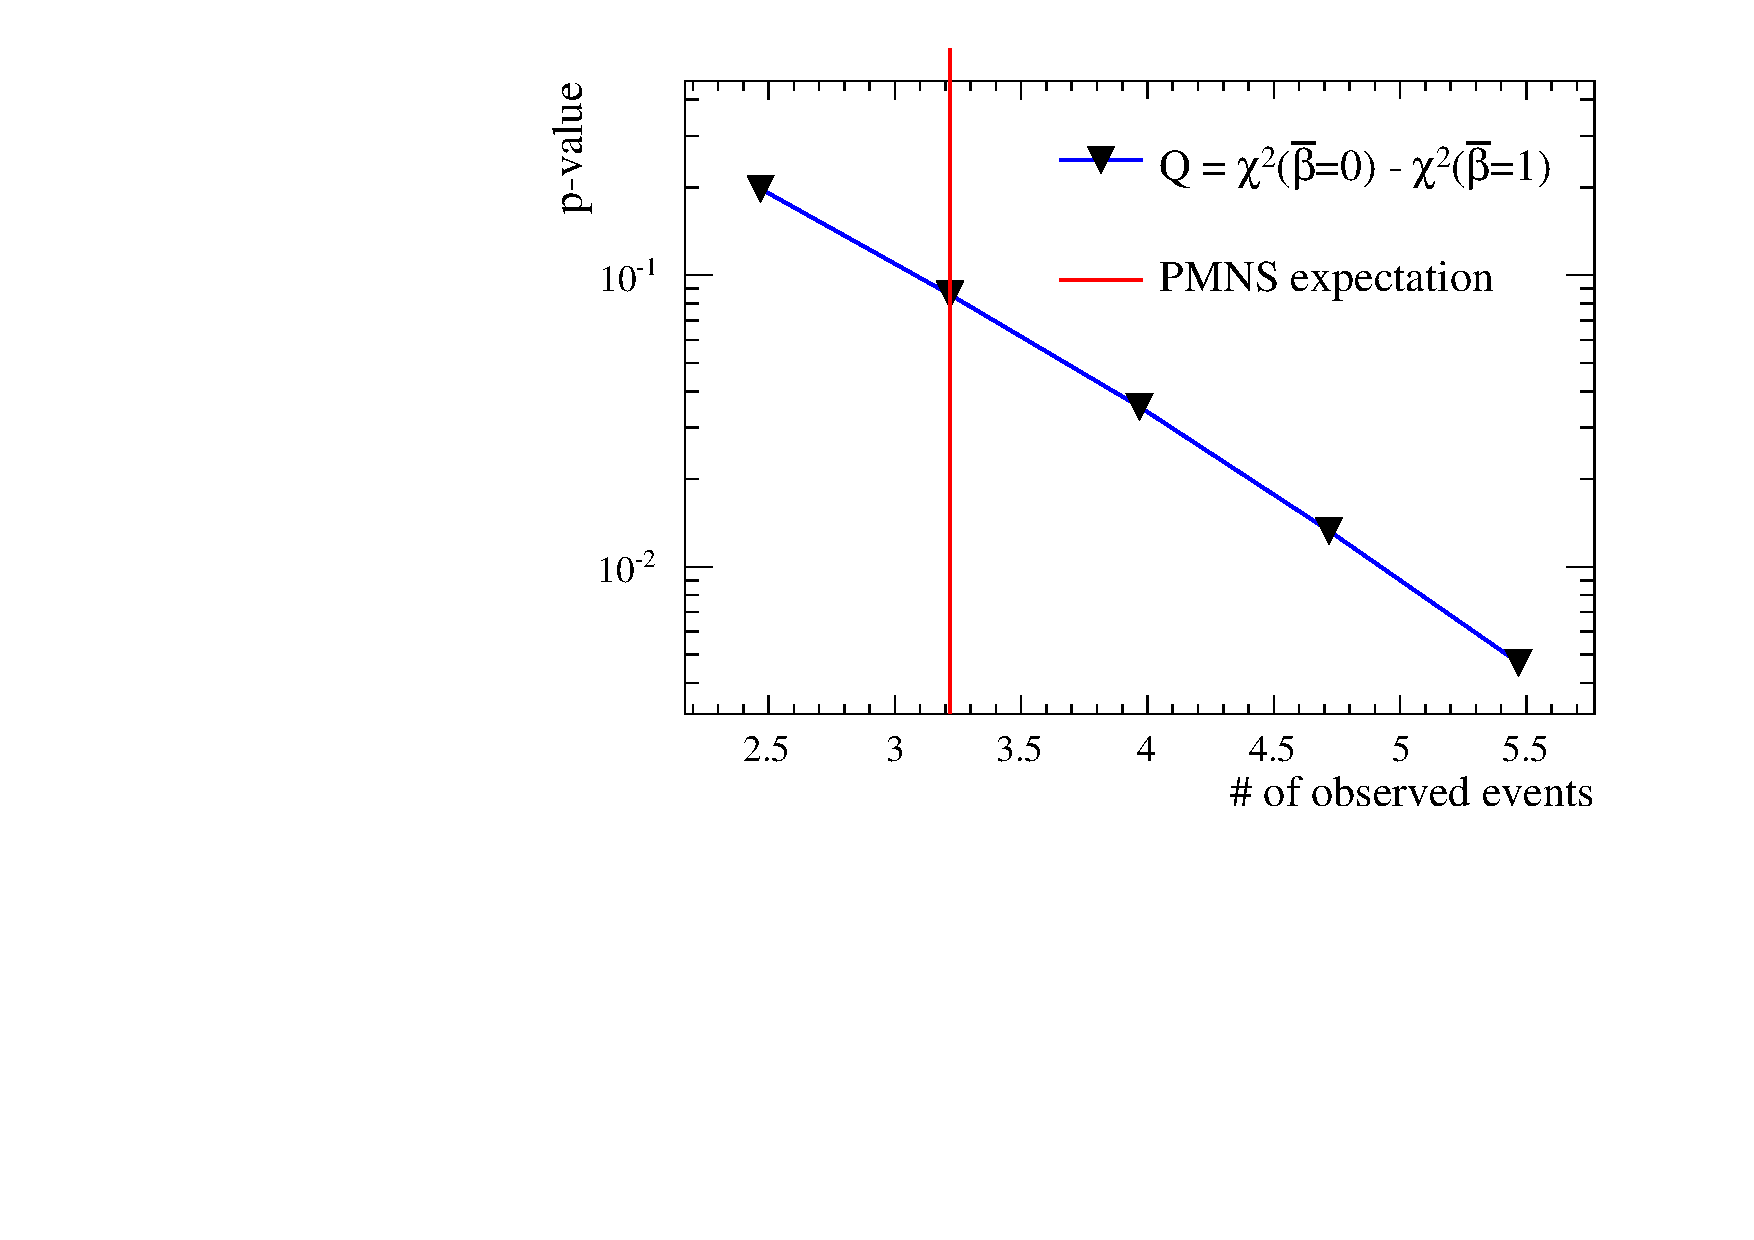
\includegraphics[width=0.9\linewidth]{./joint_plots/nuebar/rateshape/pvalue_Vs_nevt_ratepshape_log.pdf}
\caption{Something else}
\end{subfigure}
\caption {
%{\huge TO UPDATE} 
Rate-only (violet) and rate+shape (blue) p-value given by Asimov datasets for several values of $\beta$
in normal (left) and logarithmic (right) scale.
The red line corresponds to the PMNS expectation ($\beta =1$).
The study is done simulating the Run 1-6 statistic.
\NumToysLarge toys are used.
}
\label{fig:pvalue_Vs_beta_lowpot}
\end{figure}

\begin{figure}
\center
\begin{subfigure}[b]{0.49\textwidth}
\center
%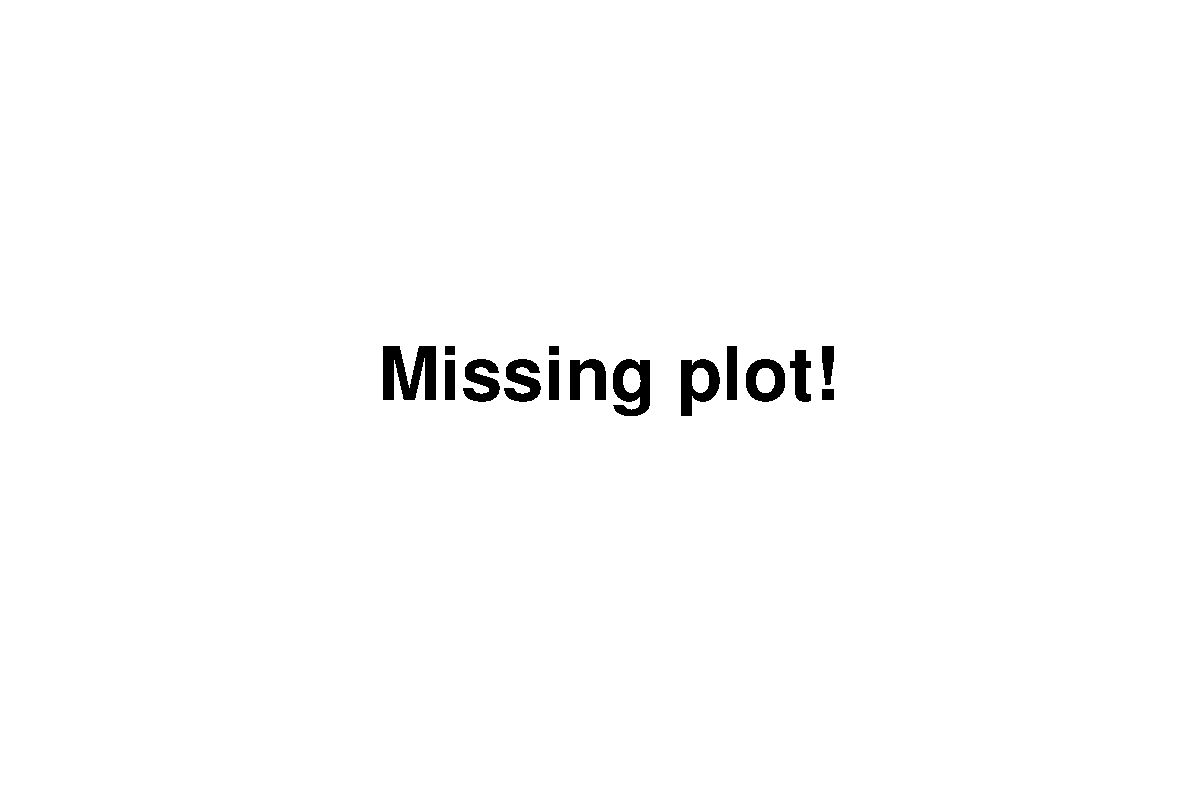
\includegraphics[width=0.9\textwidth]{./images/missing_plot-eps-converted-to.pdf}
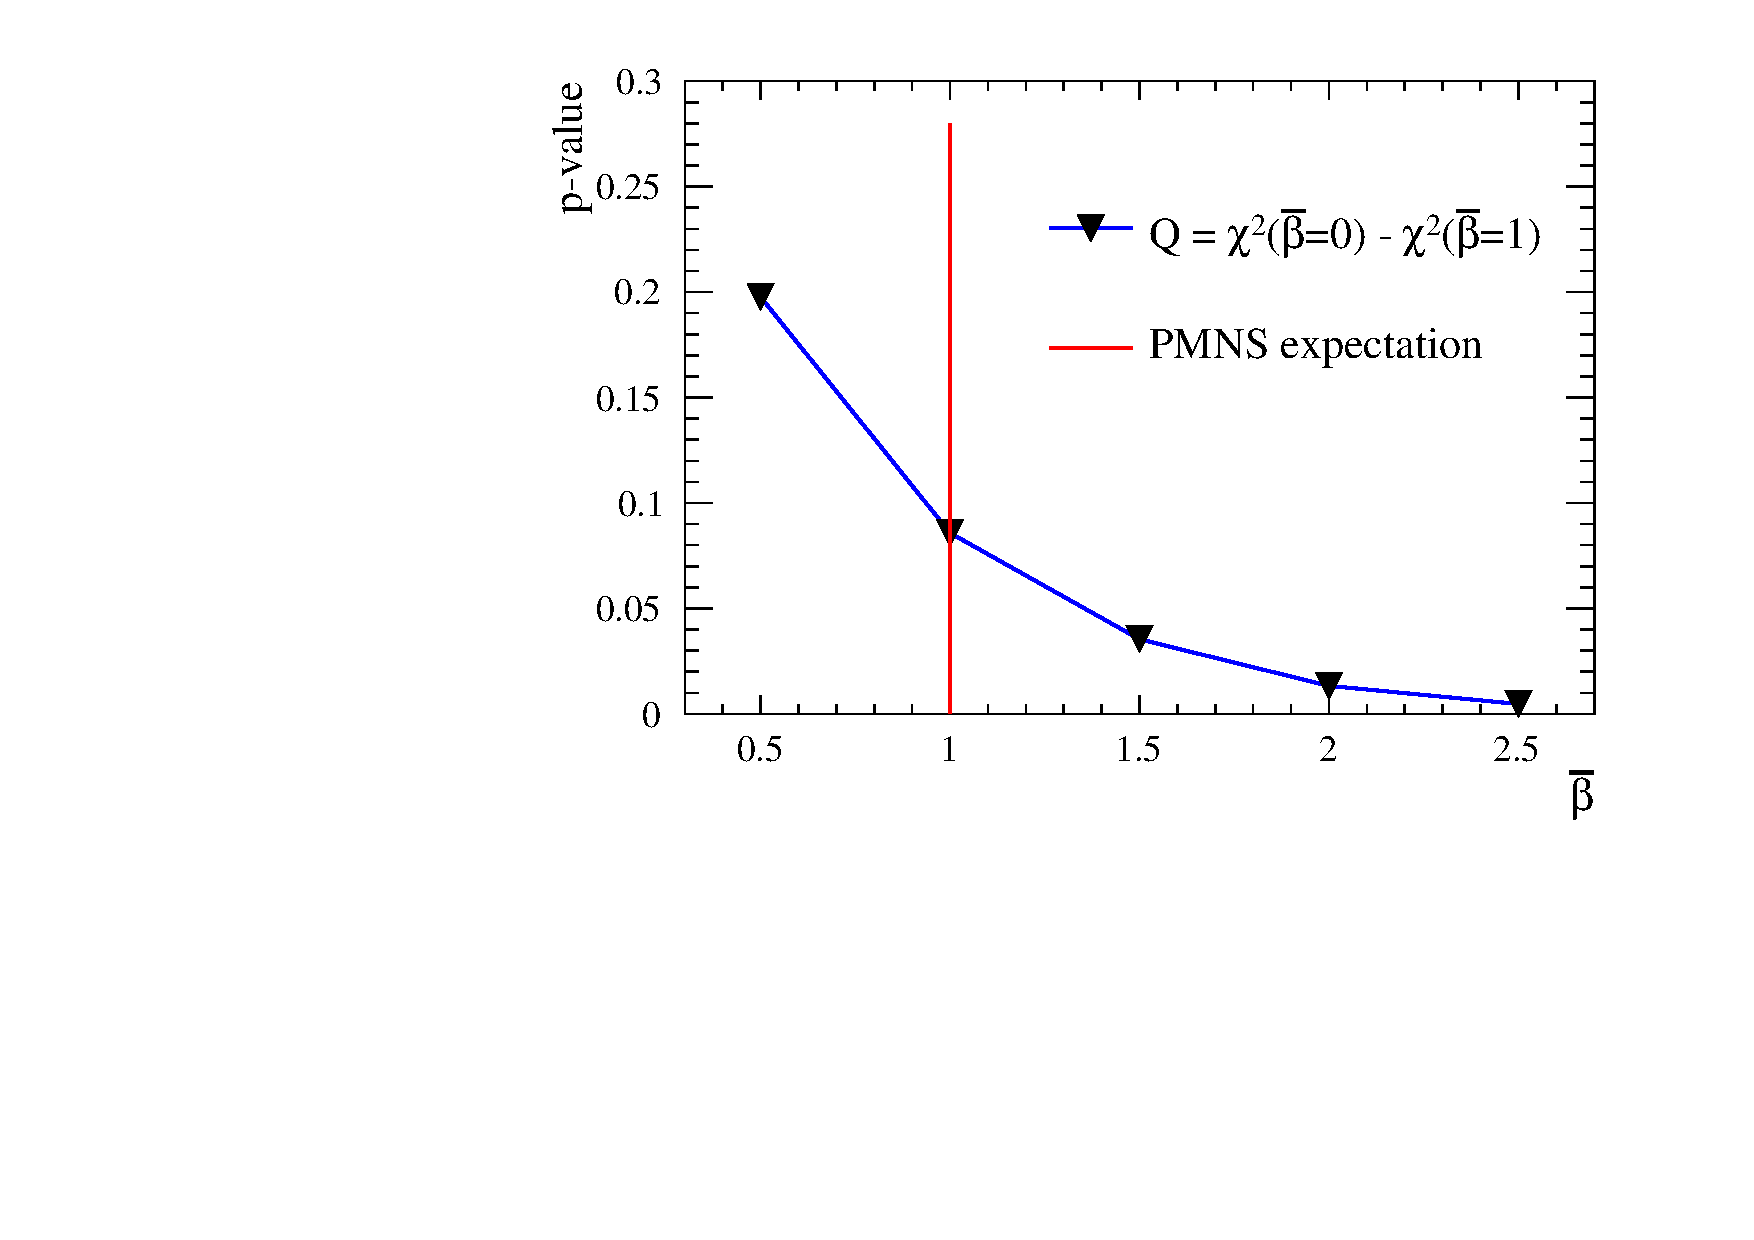
\includegraphics[width=0.9\linewidth]{./joint_plots/nuebar/rateshape/pvalue_Vs_betabar_ratepshape.pdf} 
\caption{Something}
\end{subfigure}
\begin{subfigure}[b]{0.49\textwidth}
\center
%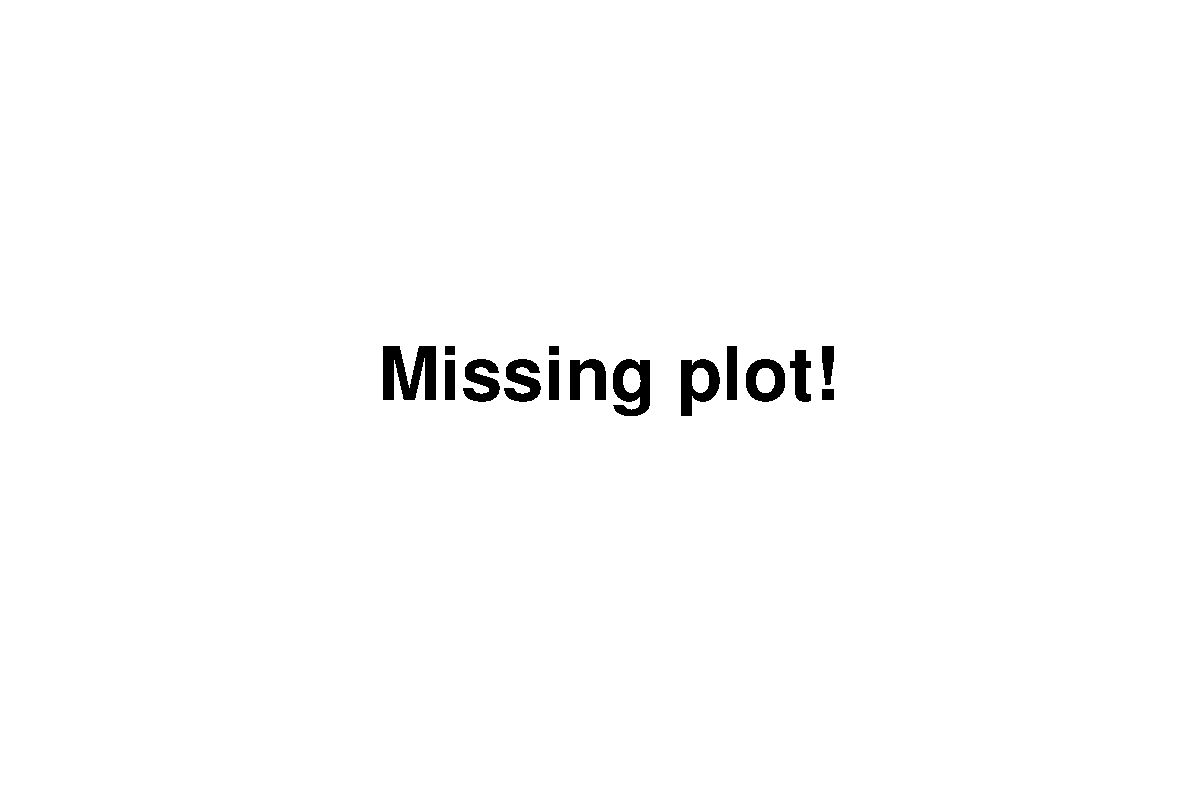
\includegraphics[width=0.9\textwidth]{./images/missing_plot-eps-converted-to.pdf}
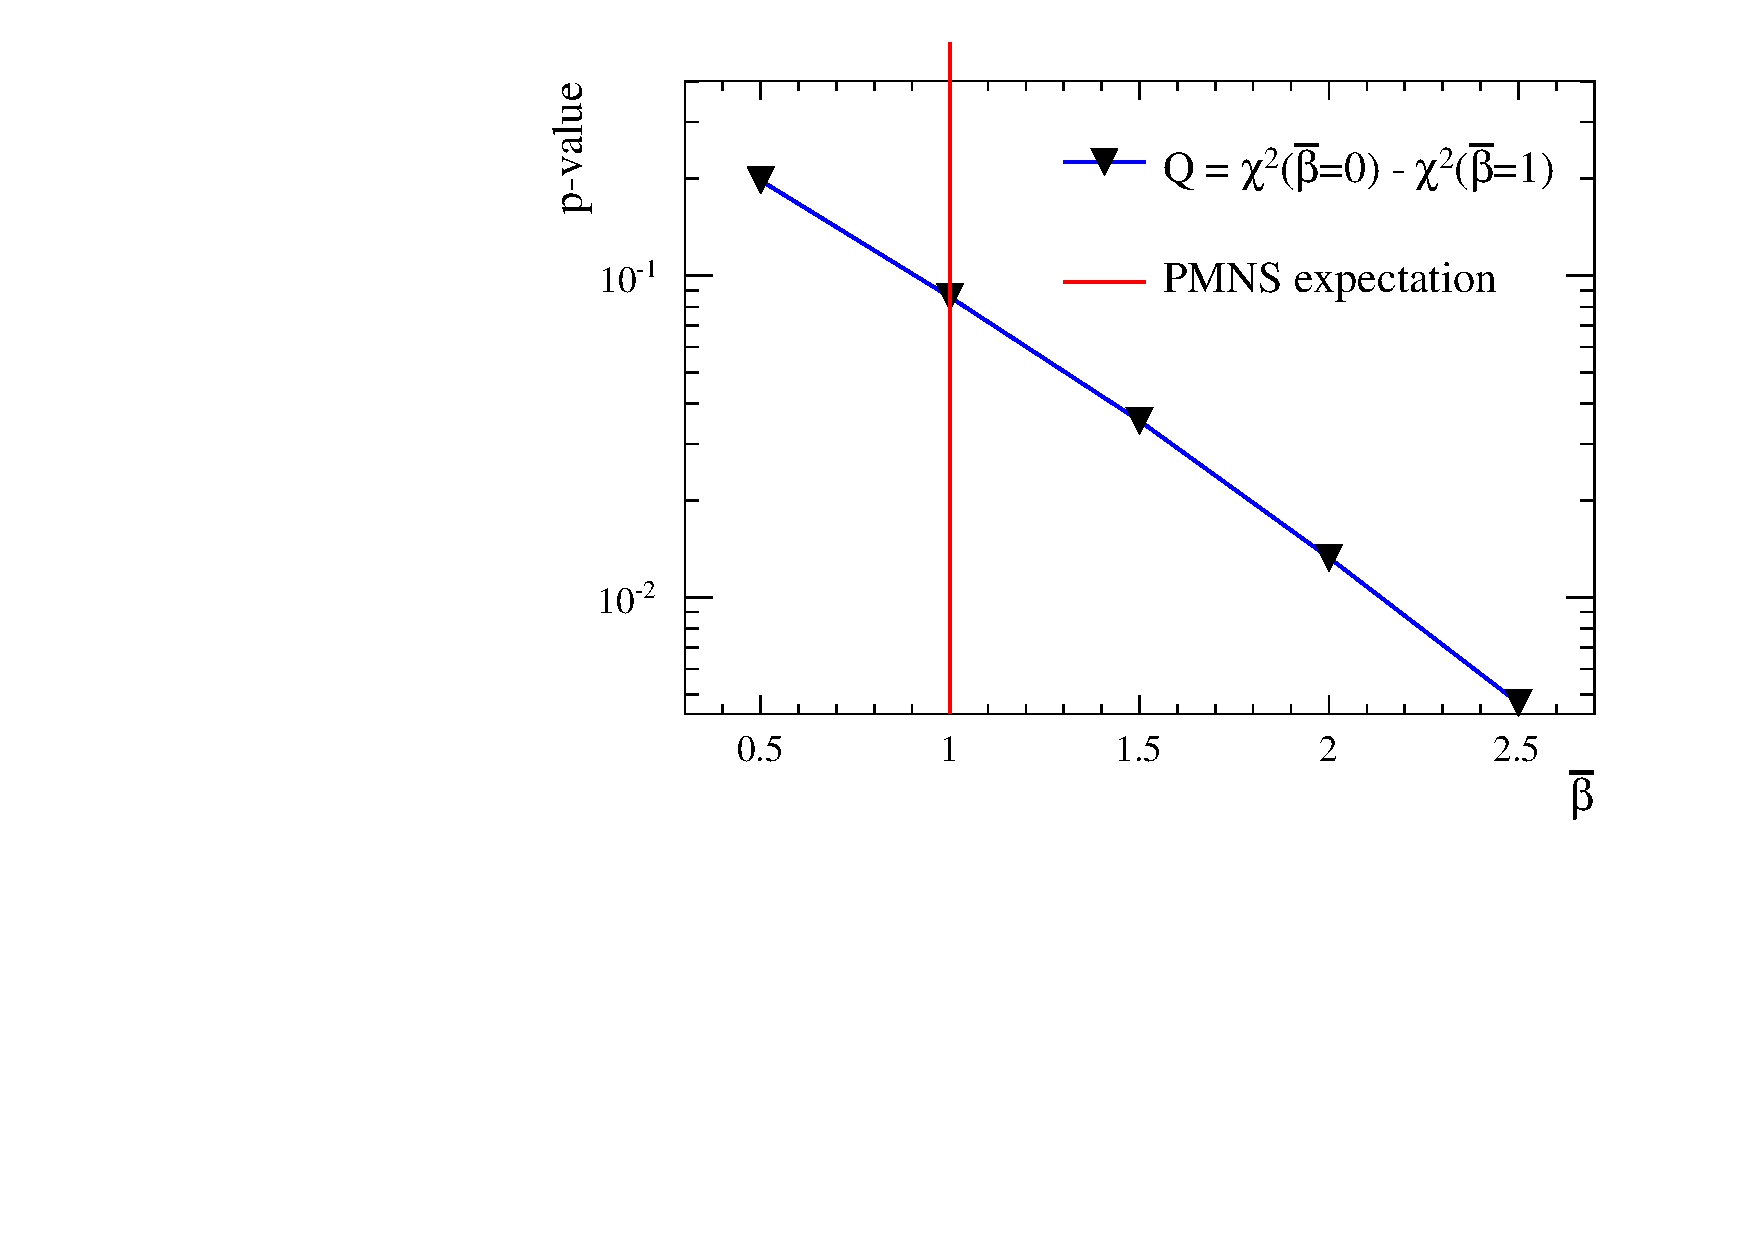
\includegraphics[width=0.9\linewidth]{./joint_plots/nuebar/rateshape/pvalue_Vs_betabar_ratepshape_log.pdf}
\caption{Something else}
\end{subfigure}
 \caption {
%{\huge TO UPDATE} 
Rate-only (violet) and rate+shape (blue) p-value for different number of observed events 
given by Asimov datasets corresponding to the several values of $\beta$ shown in \cref{fig:pvalue_Vs_beta_lowpot}.
Both normal (left) and logarithmic scales (right) are shown.
The red line corresponds to the PMNS expectation ($\beta =1$).
The study is done with Run 1-6 statistic. 
\NumToysLarge toys are used.
}
\label{fig:pvalue_Vs_nevents_lowpot}
\end{figure}


%\begin{figure}
%\center
%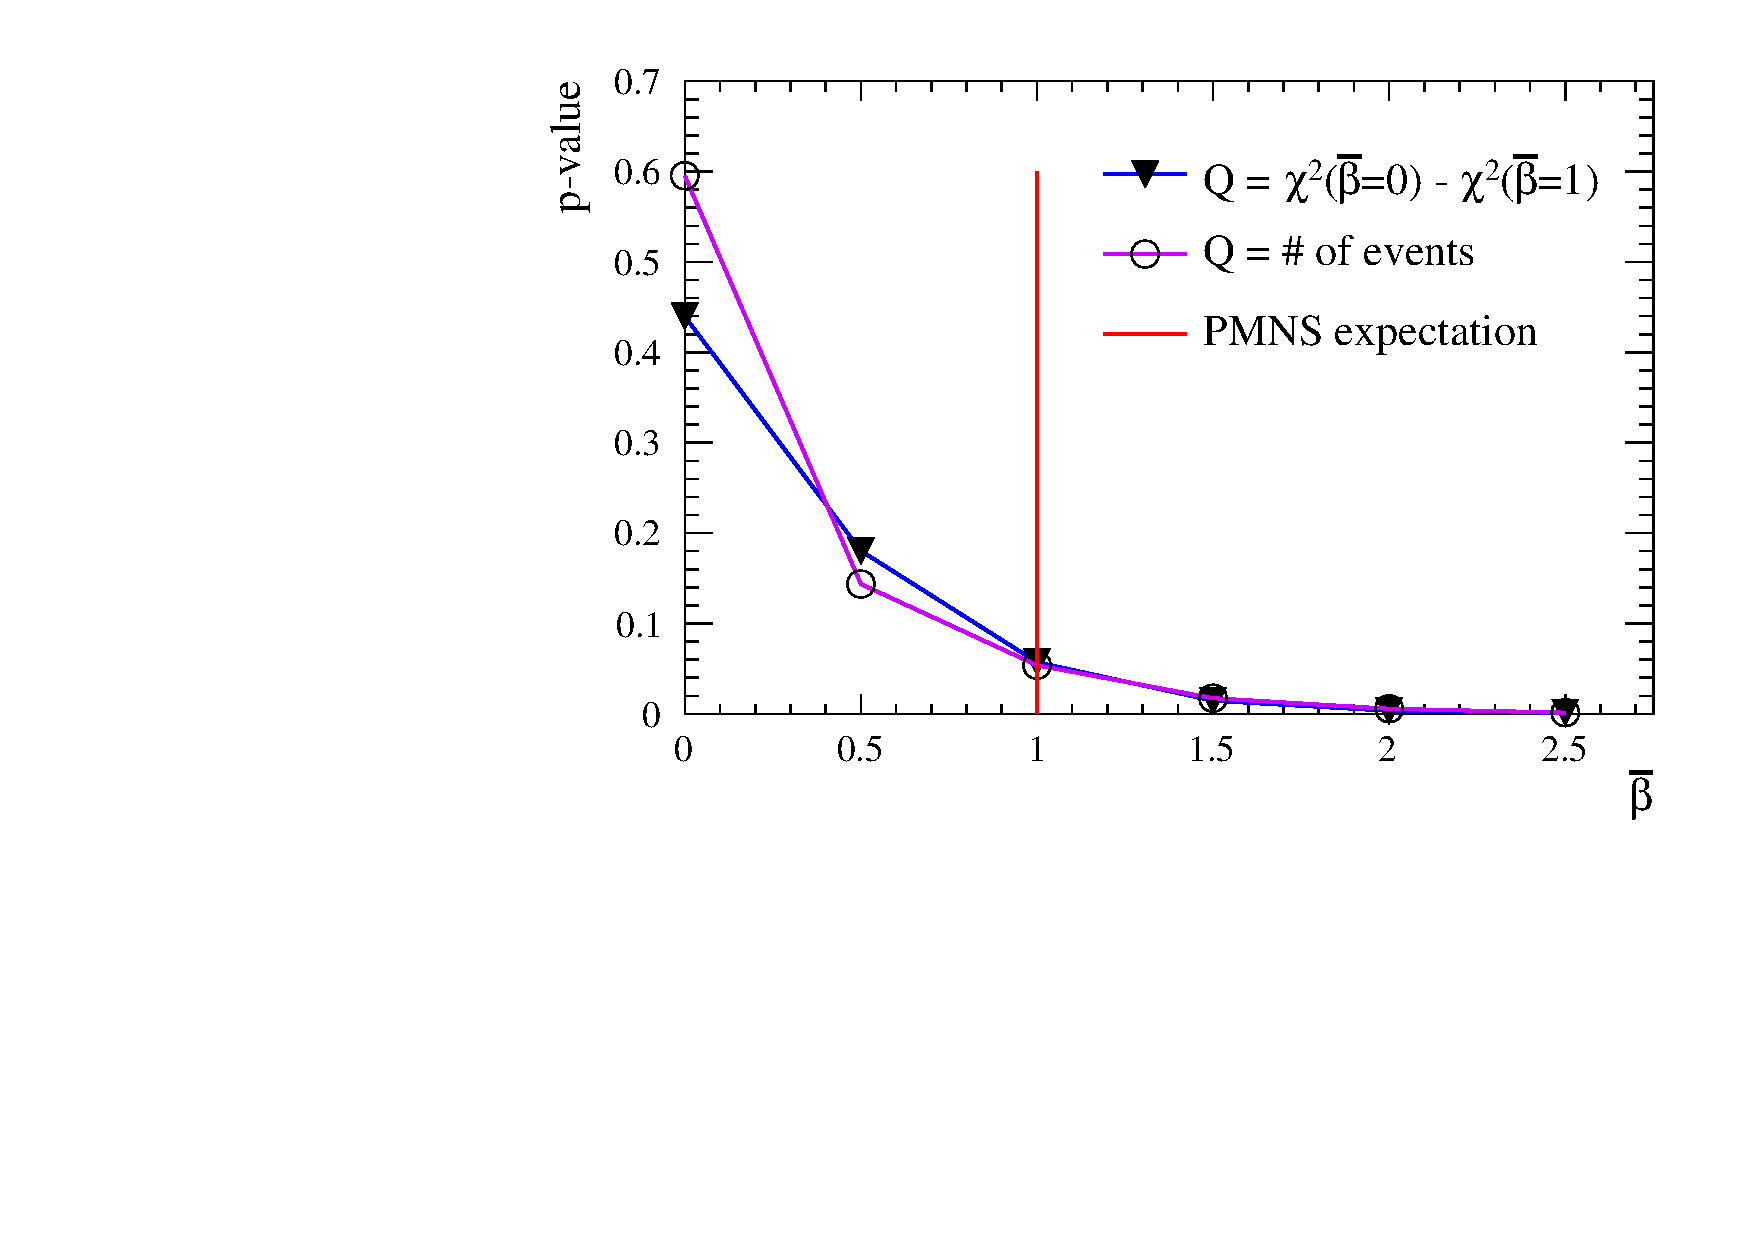
\includegraphics[width=0.48\linewidth]{./nuebar_plots/sensitivity/pvalue_Vs_beta_4p5E20POT.pdf}
%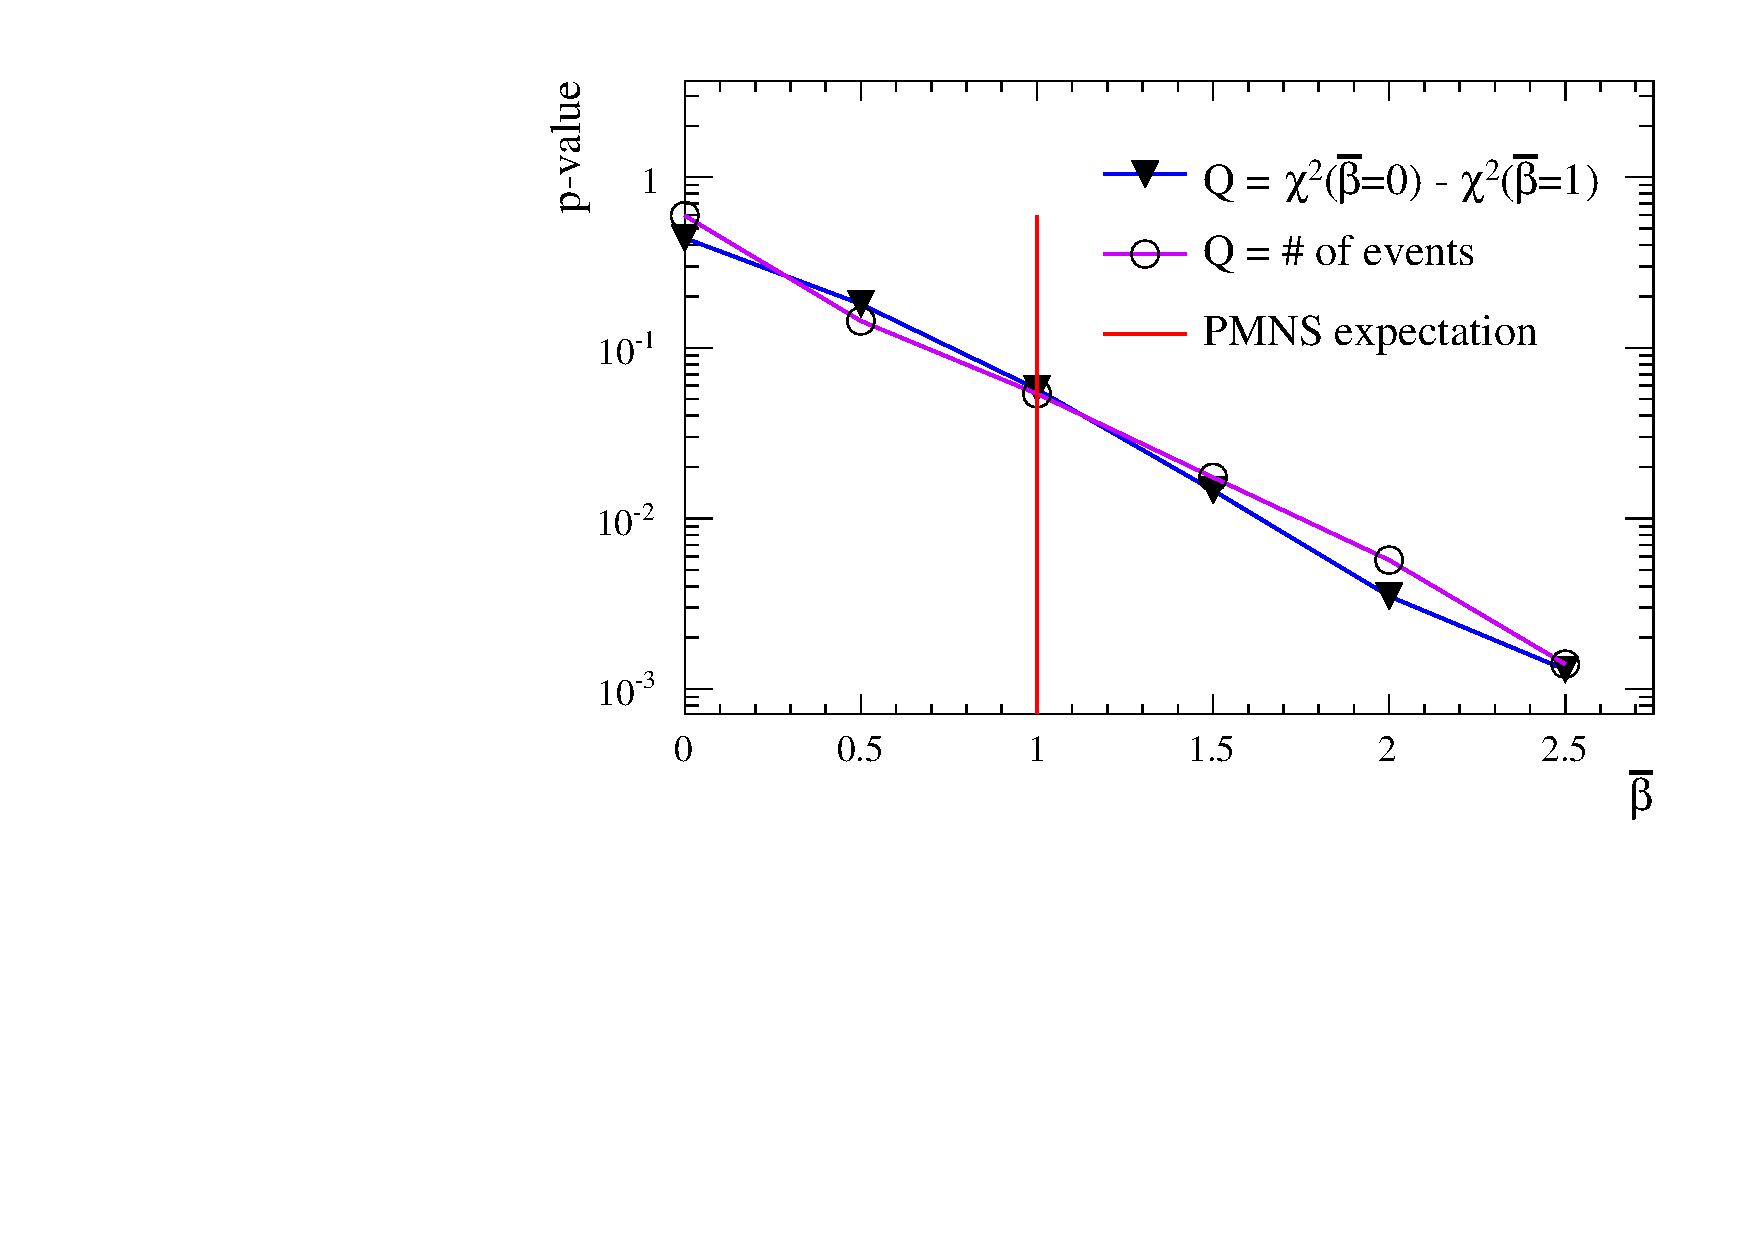
\includegraphics[width=0.48\linewidth]{./nuebar_plots/sensitivity/pvalue_Vs_beta_4p5E20POT_log.pdf}
%\caption {
%Rate-only (violet) and rate+shape (blue) p-value given by Asimov datasets for several values of $\beta$
%in normal (up) and logarithmic (bottom) scale.
%The red line corresponds to the PMNS expectation ($\beta =1$).
%The study is done with 
%\FakePotHigh POT.
%%\newline
%%{\bf TO UPDATE}
%%\newline
%}
%\label{fig:pvalue_Vs_beta_highpot}
%\end{figure}
%
%\begin{figure}
%\center
%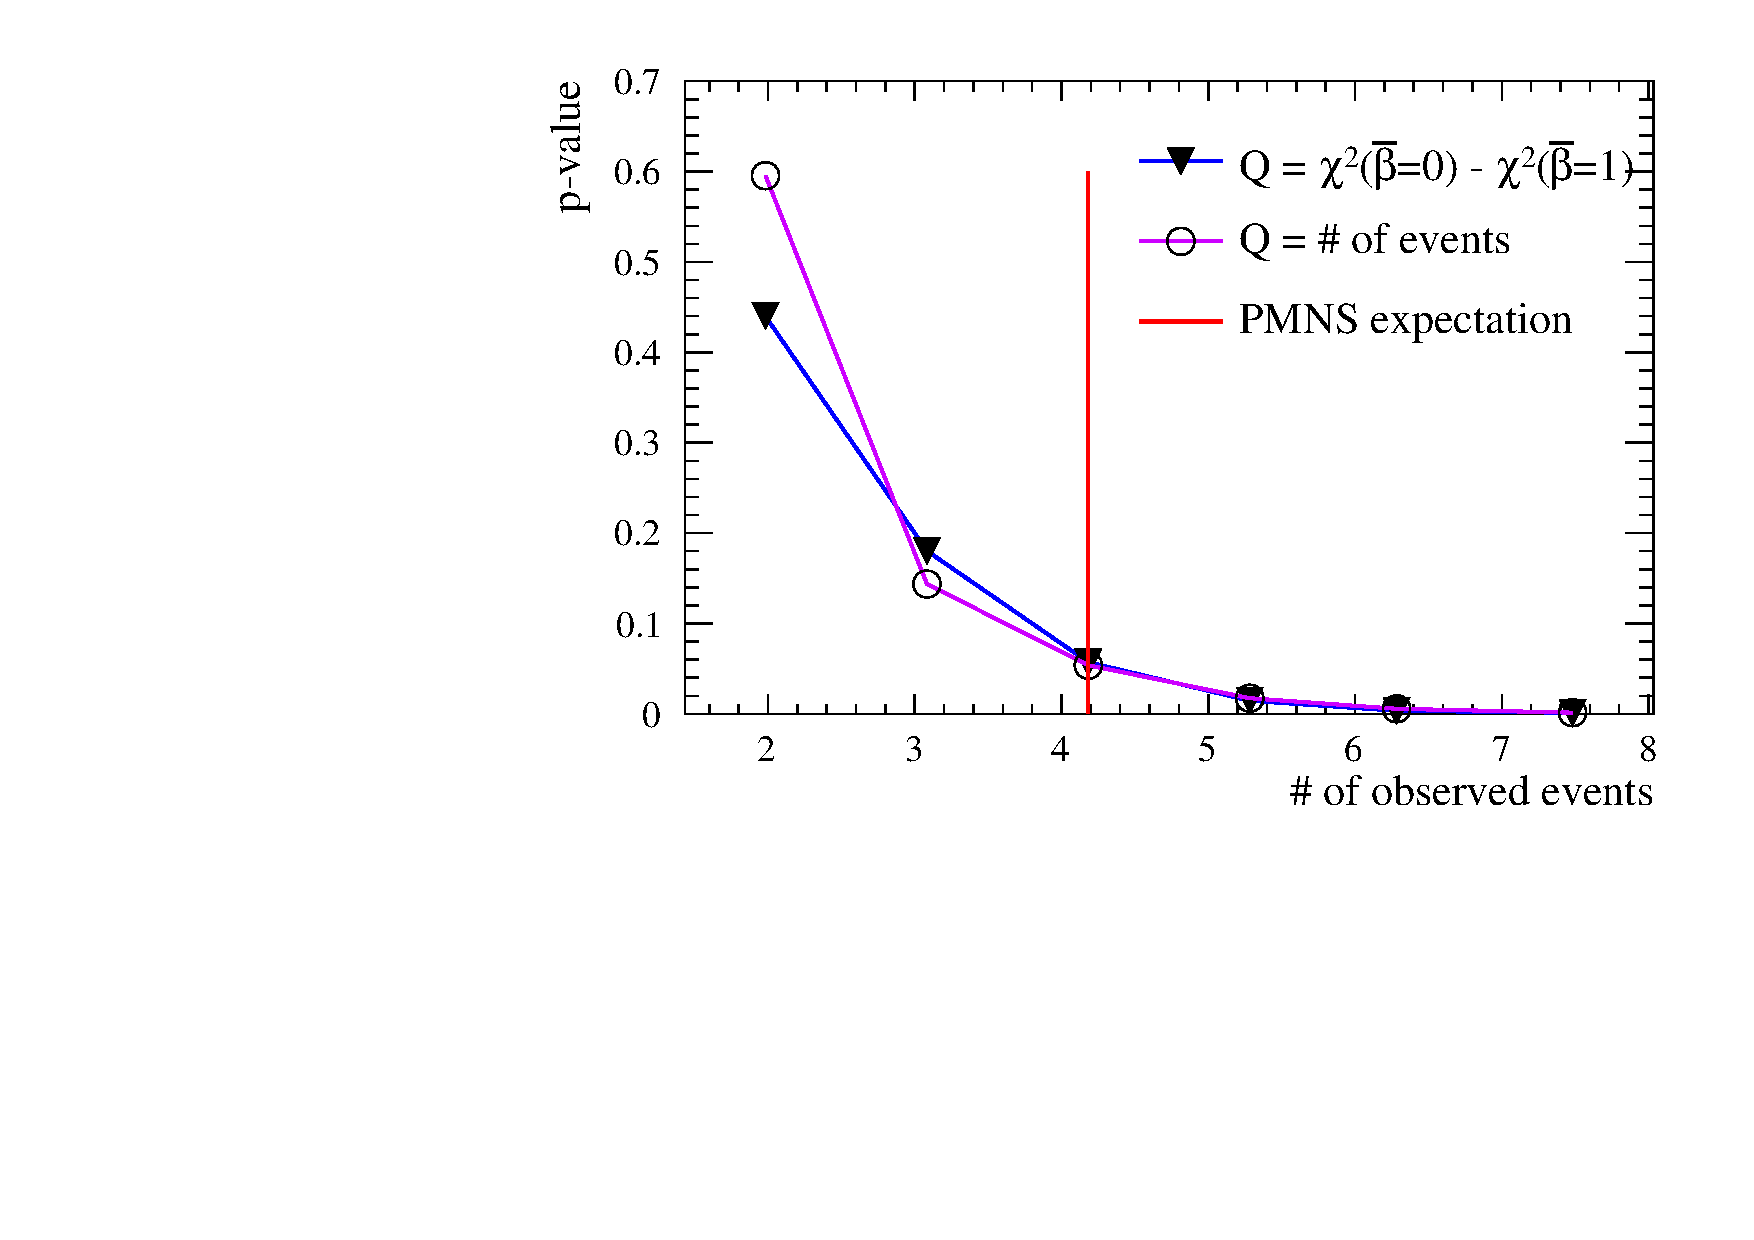
\includegraphics[width=0.48\linewidth]{./nuebar_plots/sensitivity/pvalue_Vs_nevents_4p5E20POT.pdf}
%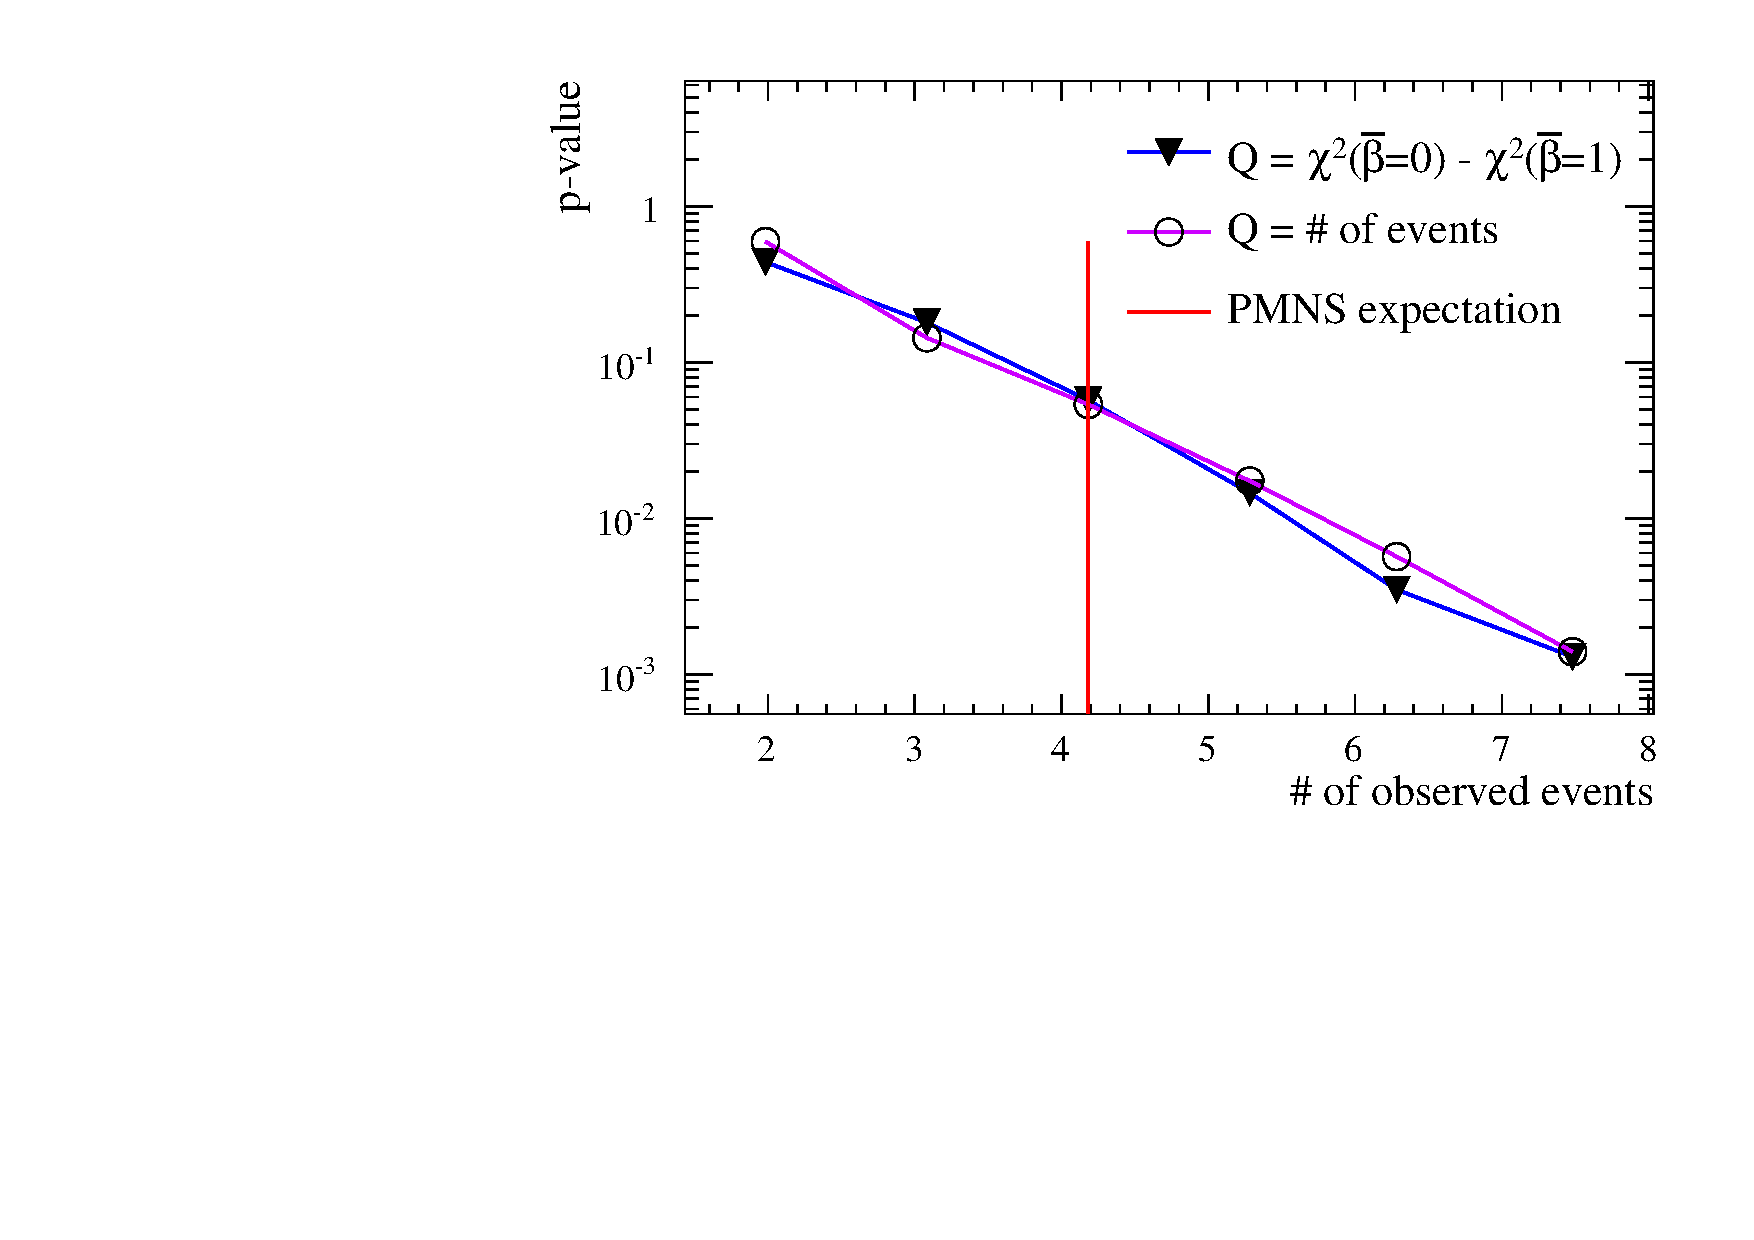
\includegraphics[width=0.48\linewidth]{./nuebar_plots/sensitivity/pvalue_Vs_nevents_4p5E20POT_log.pdf}
%\caption {
%Rate-only (violet) and rate+shape (blue) p-value for different number of observed events 
%given by Asimov datasets corresponding to the several values of $\beta$ shown in \cref{fig:pvalue_Vs_beta_highpot}.
%Both normal (up) and logarithmic scales (bottom) are shown.
%The red line corresponds to the PMNS expectation ($\beta =1$).
%The study is done with 
%\FakePotHigh POT.
%%\newline
%%{\bf TO UPDATE}
%%\newline
%}
%\label{fig:pvalue_Vs_nevents_highpot}
%\end{figure}


%--------------------------------------------------------------------------------------------------------------------

\subsection {Mean p-value}
\label{subsec:pvalue_mean}

The mean p-value is computed without using the Asimov dataset, but with toy experiments:
\begin{itemize}
\item the distributions shown in \cref{fig:pvalue_rateonly} and \cref{fig:pvalue_rateshape} 
	are used respectively for the rate-only and rate+shape p-value computations,
\item \NumToysLarge toys are produced with $\beta = 1$, 
\item for each toy with $\beta=1$ the test statistic (i.e. the number of events and 
	$\Delta \chi^2$ given in \cref{eq:deltachisq_rateshape})
	is computed and a 1-sided p-value (right tail) is quoted using the distributions 
	\cref{fig:pvalue_rateonly} and \cref{fig:pvalue_rateshape}, 
\item a distribution of rate-only and rate+shape p-values is obtained and the mean p-value is calculated.
\end{itemize}

The mean rate-only p-value, given by the mean of the p-value distribution shown in \cref{fig:pvalue_mean}, is XXX
while the mean rate+shape p-value is 0.170 for 
Run 1-6 statistic.
%\TotalPot POT.
%\FakePotLow POT.
%For \FakePotHigh POT the rate-only p-value is 0.188 while the rate+shape is 0.127.
%For both cases 
The mean p-value is larger than the Asimov one, which corresponds to the most probable p-value. 
It is worth to point out that sometimes it can happen that the rate-only
p-value is smaller than the rate+shape one. This can be due to both the discreteness of the rate-only
p-value or to the shape information wich can discard the $\bar{\nu}_e$ appearance hypothesis.
On average the rate+shape p-value is smaller than the rate-only one,
since it exploits also the shape information, but if a single dataset is used
it can happen that, due to the discreteness of test statistic (number of events), the rate-only p-value
is smaller than the rate+shape p-value.
Indeed a change of the number of events produce a not small jump in the p-value, 
as shown in the left plot of \cref{fig:pvalue_mean}, while the distribution of the 
rate+shape p-value is smooth and continuos.
For this reason it is important to quote both the p-values.
 
\begin{figure}
\center
%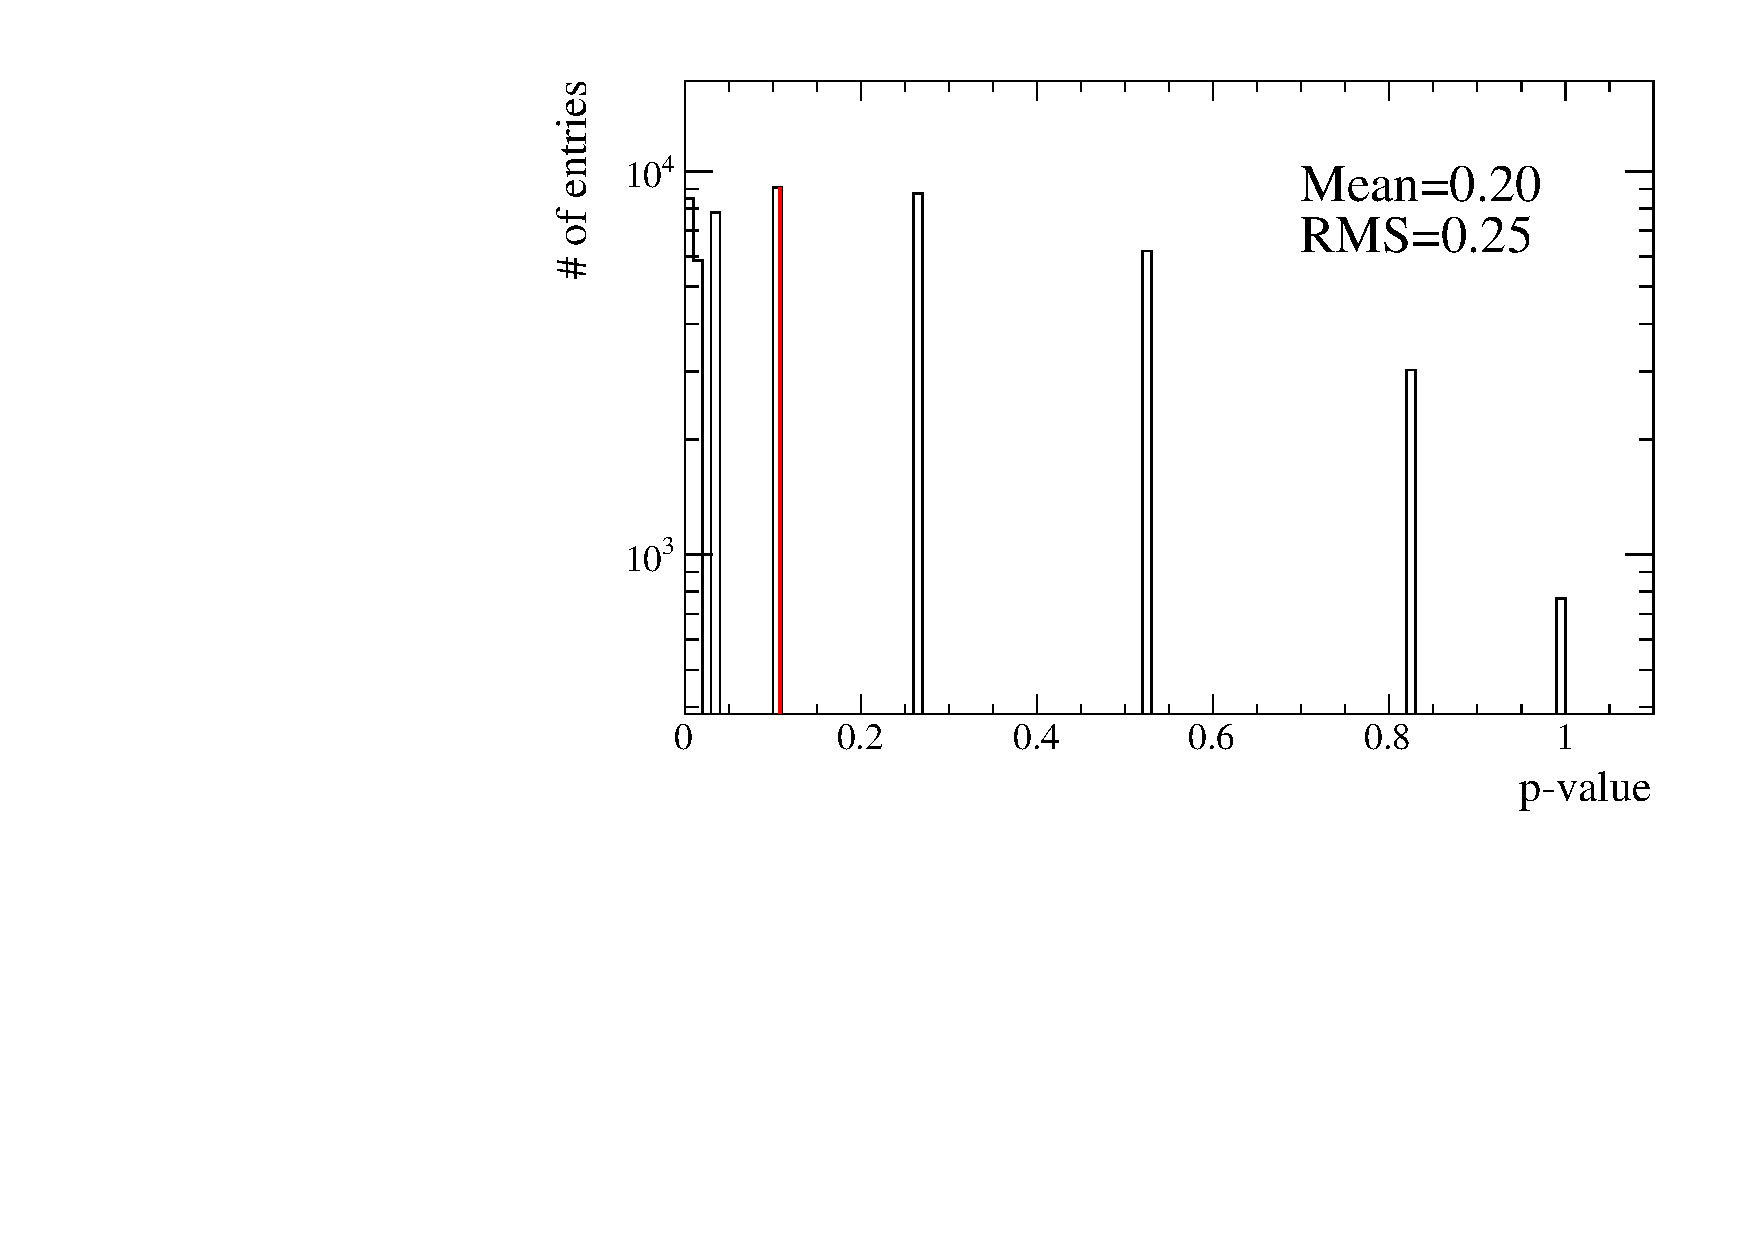
\includegraphics[width=0.48\linewidth]{./nuebar_plots/pvalue_mean/pvalue_rateonly_ave_all_4p0108E20POT_50ktoys.pdf}
\begin{subfigure}[b]{0.49\textwidth}
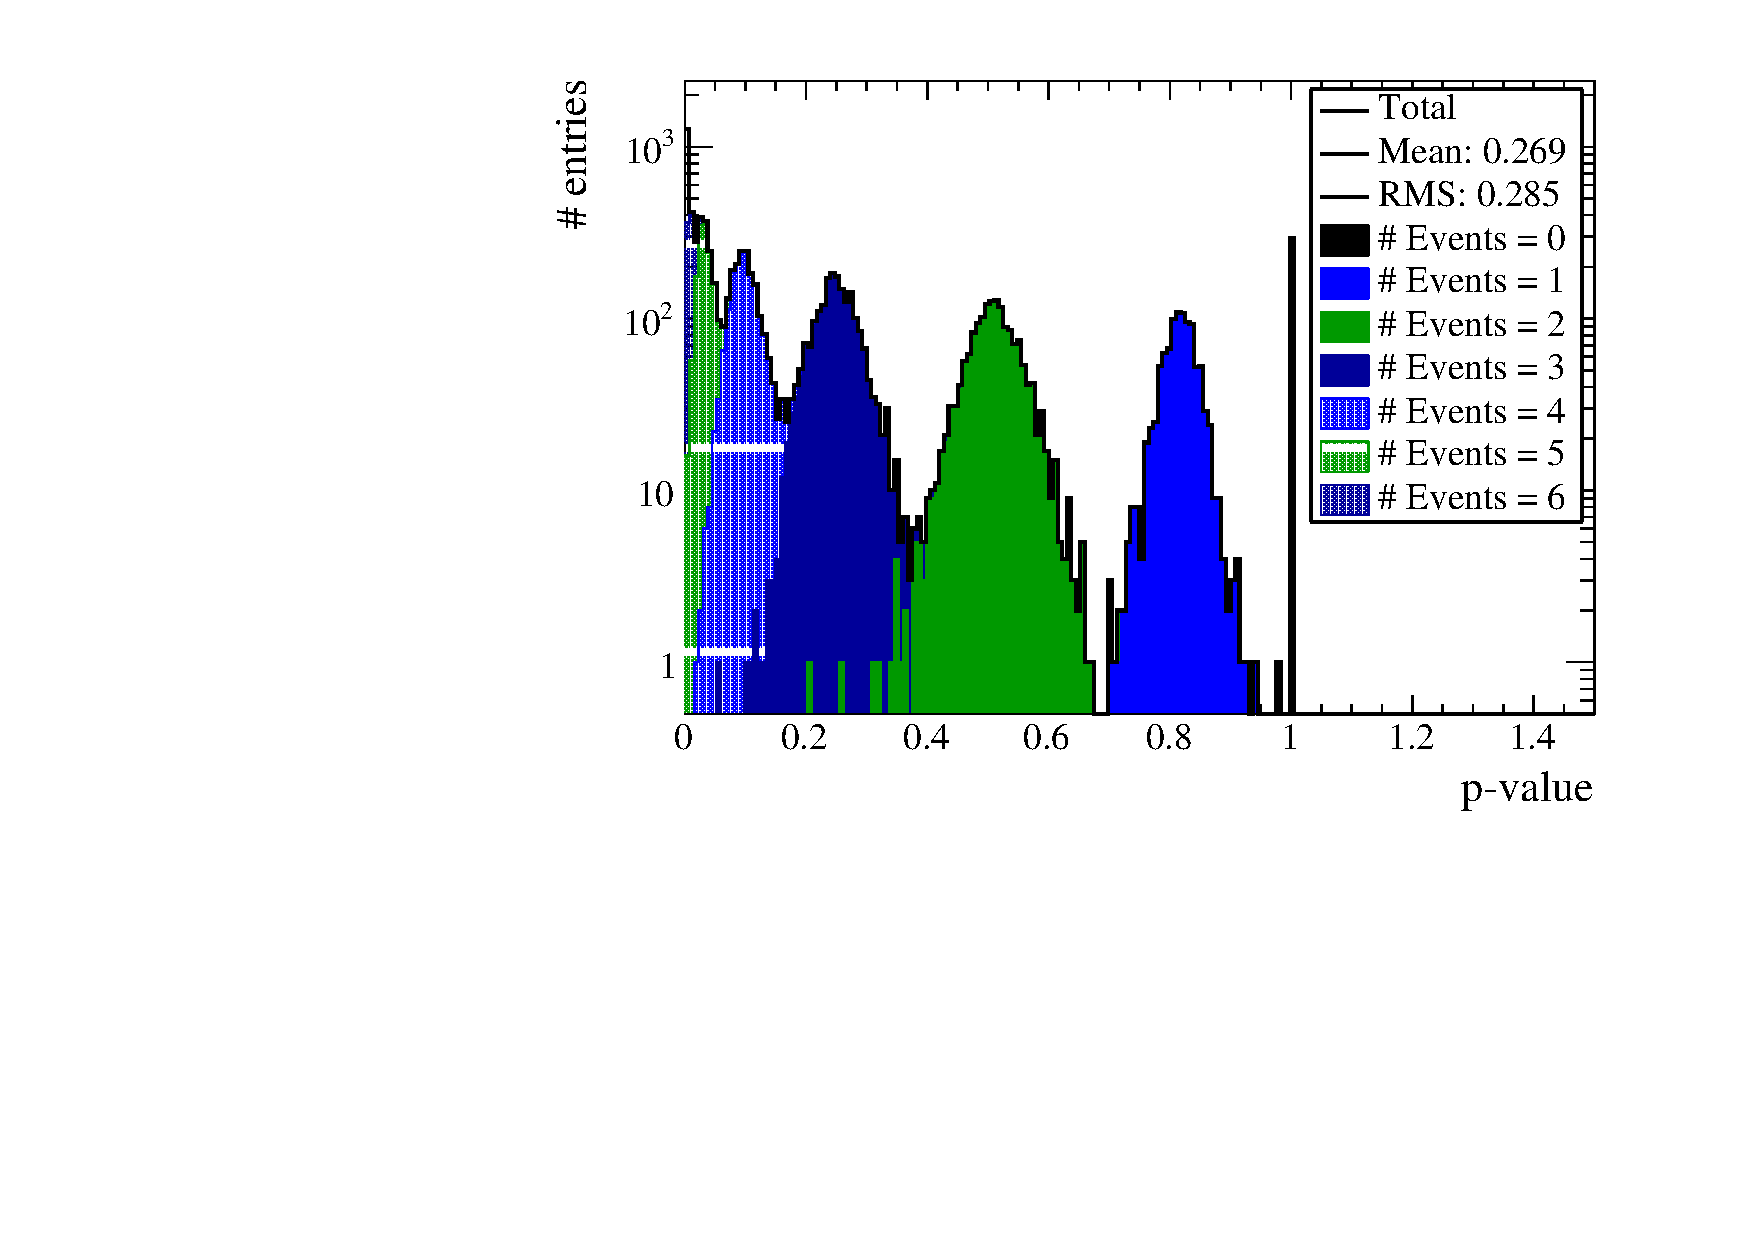
\includegraphics[width=0.9\textwidth]{./joint_plots/nuebar/rateonly/pvalue_data_beta1_dist_0.pdf}
\caption{Rate only}
\end{subfigure}
\begin{subfigure}[b]{0.49\textwidth}
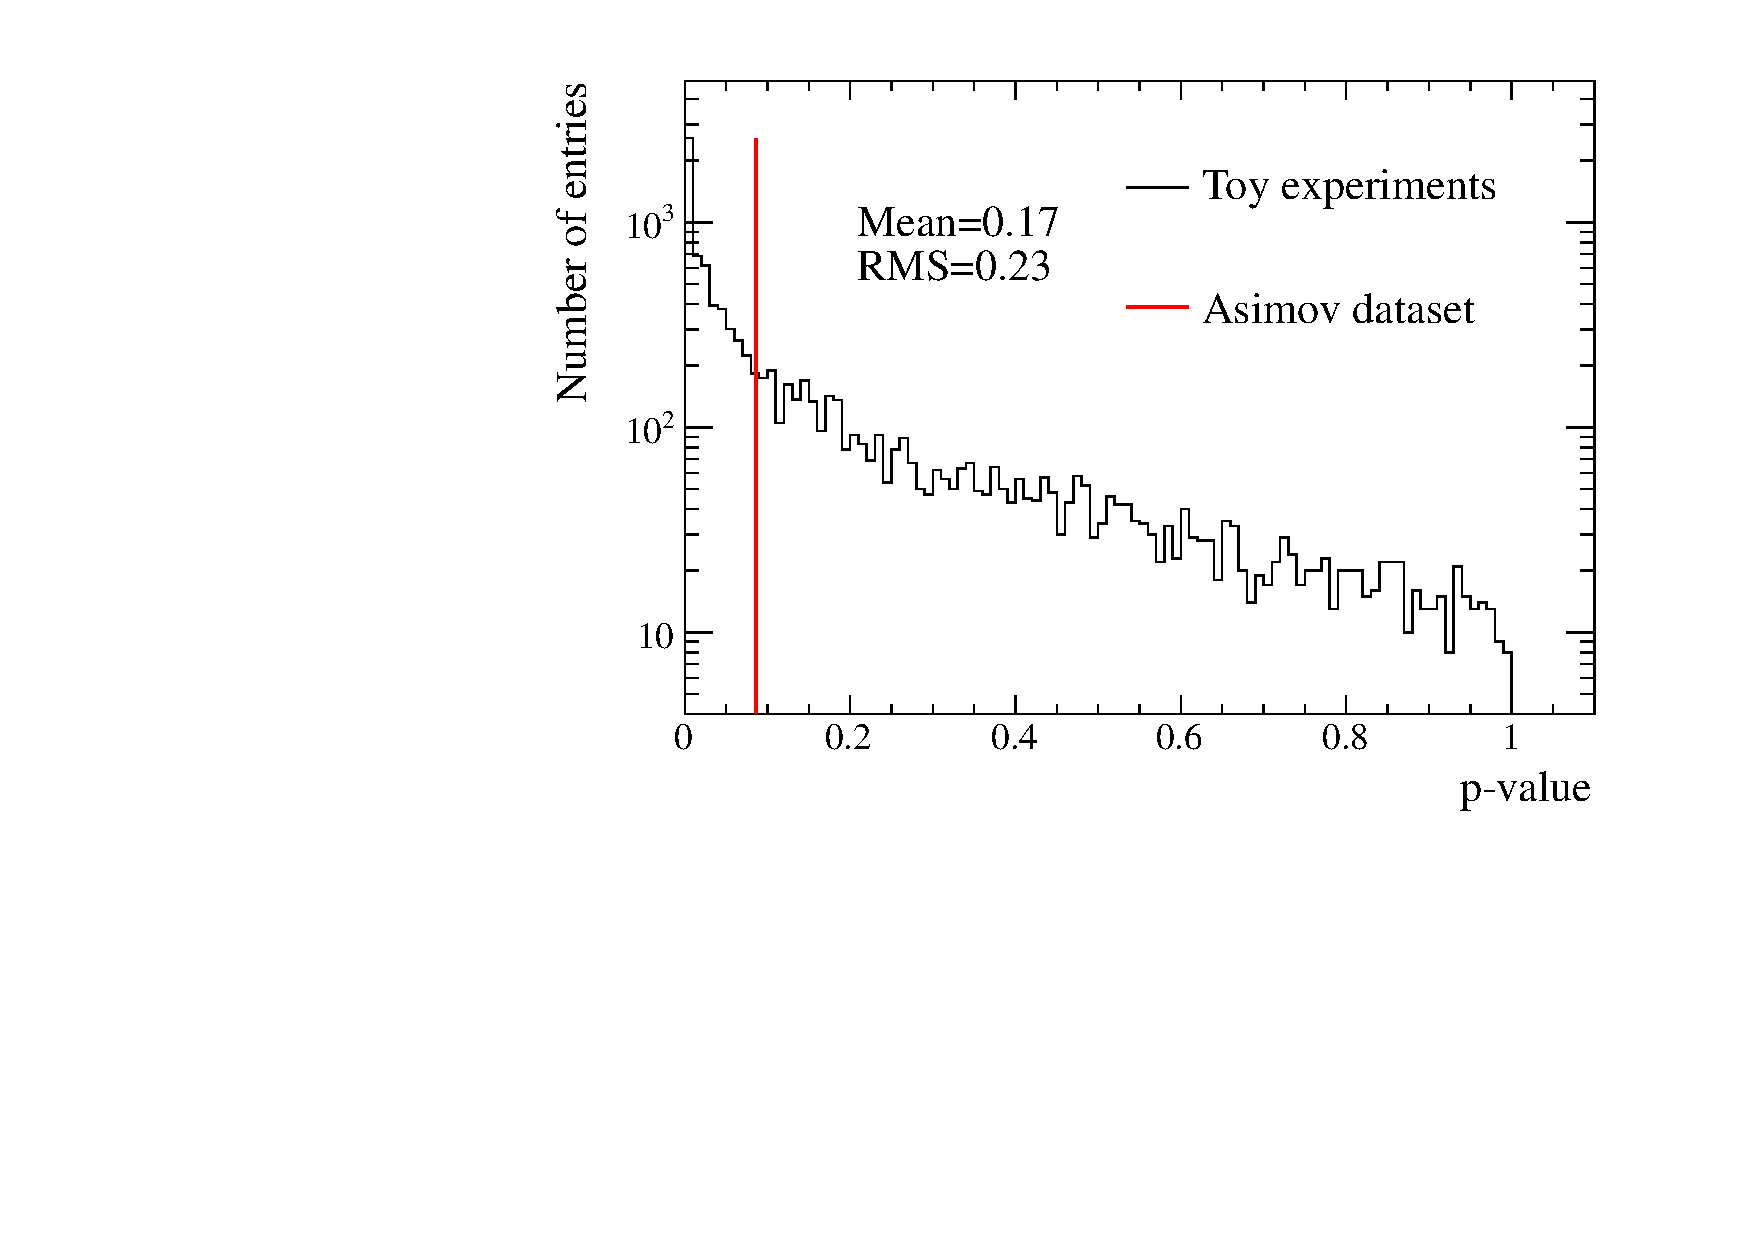
\includegraphics[width=0.9\textwidth]{./joint_plots/nuebar/rateshape/cPvalue_rateshape.pdf}
\caption{Rate + Shape}
\end{subfigure}
\caption {
%{\huge TO UPDATE} 
Distribution p-values obtained by \NumToysLarge toys with $\beta=1$.
The rate-only p-value is discrete and each filled bin correspond to toys with different number of events.
In both distributions the spike at p-value=1 corresponds to toys with no events.
The study is performed with 
Run 1-6 statistic.
\NumToysLarge toys are used.
}
\label{fig:pvalue_mean}
\end{figure}

In \cref{fig:pvalue_Vs_nevents_2Dplot} the rate+shape p-value as a function 
of the number of events for single toy produced with $\beta=1$ is shown for the Run 1-6 statistic.

\begin{figure}
\center
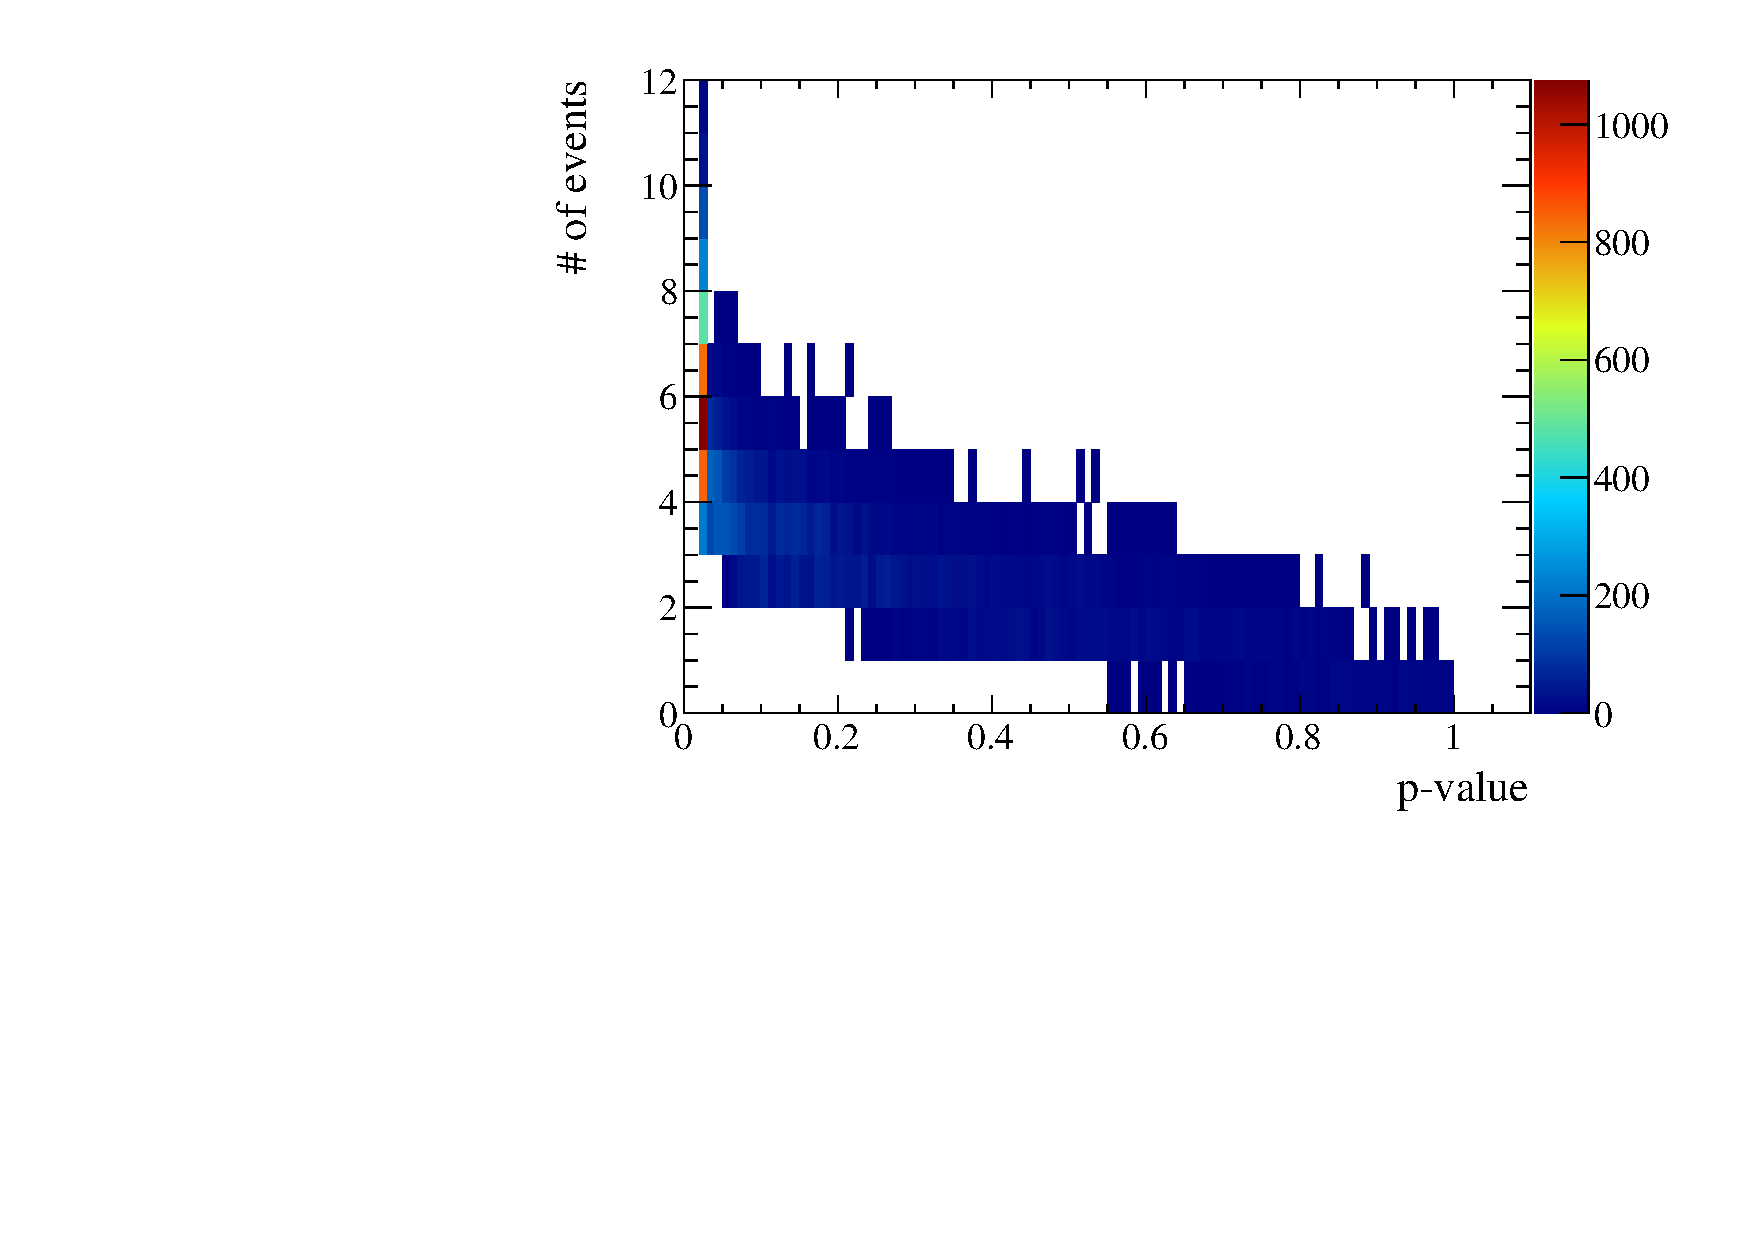
\includegraphics[width=0.6\linewidth]{./joint_plots/nuebar/rateshape/cPvalueVsNevt.pdf}
\caption {
The rate+shape p-value as a function of the number of events for a single toy produced with $\beta=1$ is shown for 
the Run 1-6 statistic.
\NumToysLarge toys are produced as described in \cref{subsec:pvalue_mean}. 
Each entry corresponds to a different toy. 
}
\label{fig:pvalue_Vs_nevents_2Dplot}
\end{figure}


%--------------------------------------------------------------------------------------------------------------------

\subsection {Summary of expected significance to $\bar{\nu}_e$ appearance}
\label{subsec:summary_sensi}

In \cref{tab:summary_sensi_lowpot} 
the expected rate-only and rate+shape p-values corresponding 
to 
Run 1-6 statistic.
In \cref{tab:summary_sensi_rateonly}
the expected rate-only p-value is shown for different number of observed events
for
Run 1-6 statistic.

%In \cref{tab:summary_sensi_manytoys_4p0108E20POT} and \cref{tab:summary_sensi_manytoys_8E20POT}
%the Asimov and Mean p-values are shown for both 
%Run 1-6 statistic 
%and $8\times 10^{20}$ POT.
%It can be seen that the expected p-value is very close to the one computed with \NumToysLarge toys.



\begin{table}
\centering
\begin{tabular}{| c | c | c |}
\hline
\# of observed events	                        	& Rate only      & Rate + Shape		    	\\
\hline
$N_{obs} = 2$      		                    	& 0.510          &          	\\
$ N_{obs} = 3$      		                    	& 0.251          &          	\\
$ \bf N_{obs} = 4$      		           	         & \bf 0.101     &             \\
$N_{obs} = 5$      		                    	& 0.0343        &        	\\
$N_{obs} = 6$      		                    	& 0.0103        &        	\\
\hline
\end{tabular}
\caption{
Summary of the expected rate-only p-values for different number of 
observed events. The simulated number of POT corresponds to Run 1-6.
\NumToysLarge toys are used to get the distribution of the test statistic and the 
Asimov data is used to compute the p-value.
The Asimov dataset for $\beta=1$ is in bold.
}
\label{tab:summary_sensi_rateonly}
\end{table}




\begin{table}
\centering
\begin{tabular}{| c | c | c |}
\hline
P-value	                                          	& Asimov    	& Mean 		    	\\
\hline
Rate-only                          			& 0.109           	& 0.269                  	\\
Rate+shape                          		& 0.0858          	& 0.170                 	\\
\hline
\end{tabular}
\caption{
Summary of the expected rate-only and rate+shape p-values for 
the Run 1-6 statistic.
The Asimov p-value is calculated using the Asimov dataset while the 
mean p-value is calculated making \NumToysLarge toys and taking the mean 
of the p-value distribution.
}
\label{tab:summary_sensi_lowpot}
\end{table}




%% Comparison with many toys
%
%\begin{table}
%\centering
%\begin{tabular}{| c | c | c |}
%\hline
%P-value	                                          			& Asimov    	  & Mean 		    	\\
%\hline
%Rate-only (\NumToys toys)         			& 0.110           & 0.207                  	\\
%Rate+shape (\NumToys toys)              		& 0.0726          & 0.143                  	\\
%\hline
%Rate-only (\NumToysLarge toys)        		& 0.109           & 0.203                	\\
%Rate+shape (\NumToysLarge toys)             	& 0.0699          & 0.139                	\\
%\hline
%\end{tabular}
%\caption{
%Summary of the expected rate-only and rate+shape p-values for 
%the Run 1-6 statistic, using \NumToys (up) and \NumToysLarge (bottom) toys for fake datasets (both $\beta=0$ and $\beta=1$).
%The Asimov p-value is calculated using the Asimov dataset while the mean one
%from \NumToys (up) and \NumToysLarge (bottom) toys and taking the mean 
%of the p-value distribution.
%}
%\label{tab:summary_sensi_manytoys_4p0108E20POT}
%\end{table}


%\begin{table}
%\centering
%\begin{tabular}{| c | c | c |}
%\hline
%P-value	                                          	& Asimov    	& Mean 		    	\\
%\hline
%Rate-only (\NumToys toys)        			& 0.0343           & 0.1004                   	\\
%Rate+shape (\NumToys toys)             		& 0.0249          	& 0.0649                 	\\
%\hline
%Rate-only (\NumToysLarge toys)        			& 0.0331           & 0.1007                   	\\
%Rate+shape (\NumToysLarge toys)             		& 0.0243          	& 0.0660                 	\\
%\hline
%\end{tabular}
%\caption{
%Summary of the expected rate-only and rate+shape p-values for 
%$8 \times 10^{20}$ POT, using \NumToys (up) and \NumToysLarge (bottom) toys for fake datasets (both $\beta=0$ and $\beta=1$).
%The Asimov p-value is calculated using the Asimov dataset while the mean one
%from \NumToys (up) and \NumToysLarge (bottom) toys and taking the mean 
%of the p-value distribution.
%}
%\label{tab:summary_sensi_manytoys_8E20POT}
%\end{table}

%





\begin{table}
\centering
\begin{tabular}{| c | c | c |}
\hline
		                                          	& p-value $\leq 0.10$    		& p-value $\leq 0.05$ 		\\
\hline
Fraction of toys	(rate-only)			& XXX\%					& XXX\%				\\
Fraction of toys	(rate+shape) 		& 58.0\%					& 46.5\%				\\
\hline
\end{tabular}
\caption{
The probability to have a p-value smaller than 0.05 and 0.10 is shown.
\NumToysLarge toys for
the Run 1-6 statistic
are produced.
Then for each toy the p-value is computed as described in section~\ref{subsec:pvalue_mean}.
}
\label{tab:pvalue_mean_0p05_lowpot}
\end{table}

\begin{table}
\centering
\begin{tabular}{| c | c | c |}
\hline
\# obs events $>$ \# exp bkg		& p-value    	 & Fraction of toys    	\\
\hline
Rate-only                          			&   XXX	    	& XXX\%             	\\
Rate+shape                          		&   0.102   	& 86.9\%                 	\\
\hline
\end{tabular}
\caption{
Summary of the expected rate-only and rate+shape mean p-values for 
the Run 1-6 statistic.
%\FakePotLow POT.
The Asimov p-value is calculated using the Asimov dataset while the 
mean p-value is calculated making \NumToysLarge toys and taking the mean 
of the p-value distribution.
Only fake datasets with number of observed events higher than the
expected background are considered.
The fraction of selected toys is shown as well. 
}
\label{tab:pvalue_mean_bkg_lowpot}
\end{table}



\begin{table}
\centering
\begin{tabular}{| c | c |}
\hline
p-value (rate-only) $>$ p-value (rate+shape)		& Probability          	\\
\hline
All toys									& XXX\%		 							\\
Toys w/ \# obs. events $>$ \# exp. bkg 			& XXX\%									\\
\hline
\end{tabular}
\caption{
The probability to have a rate-only p-value larger than the rate+shape p-value is shown.
\NumToysLarge toys for 
the Run 1-6 statistic.
%\FakePotLow POT are produced.
Then for each toy the p-value is computed as described in section~\ref{subsec:pvalue_mean}.
Both all toys are considered as well as the toys with the number of observed events larger
than the number of expected background.
}
\label{tab:pvalue_mean_rate_large_shape_lowpot}
\end{table}




The mean rate-only and rate+shape p-values, obtained considering only p-values smaller than 0.05 (0.10), 
are shown \cref{tab:pvalue_mean_0p05_lowpot}.
%The corresponding figures are shown in \cref{app:rateshape_mean_pvalue}.

In \cref{tab:pvalue_mean_bkg_lowpot}
mean p-values corresponding to 
Run 1-6 statistic
for those fake datasets with the number of observed events higher than the expected background are shown. 

In \cref{tab:pvalue_mean_rate_large_shape_lowpot} 
the probability to have the rate-only p-value smaller than the rate+shape p-value is shown for
Run 1-6 statistic


\clearpage



\section {Results of the $\bar{\nu}_{e}$-appearance analysis}
\label{sec:results_nuebar}

%--------------------------------------------------------------------------------------
% p-value
%--------------------------------------------------------------------------------------

\subsection {Significance to $\bar{\nu}_e$ appearance}
\label{sec:pvalue_nuebar}

The rate-only and rate+shape p-values for $\bar{\nu}_e$-appearance are performed
on the combined 
Run 1-6 statistic
following the same procedure as in \cref{sec:sensitivity_nuebarapp}. 
1-sided p-values are computed on the right tail of the test statistic expected distribution.
All the \NSyst{} systematic parameters are marginalised.
A summary of the observed number of events in Super-K, $\Delta \chi^{2}$ and p-values is given
in \cref{tab:results}.



%...........................................................
%
% Delta Chisq and # of events distributions with data overlapped
%

\begin{figure}
\center
%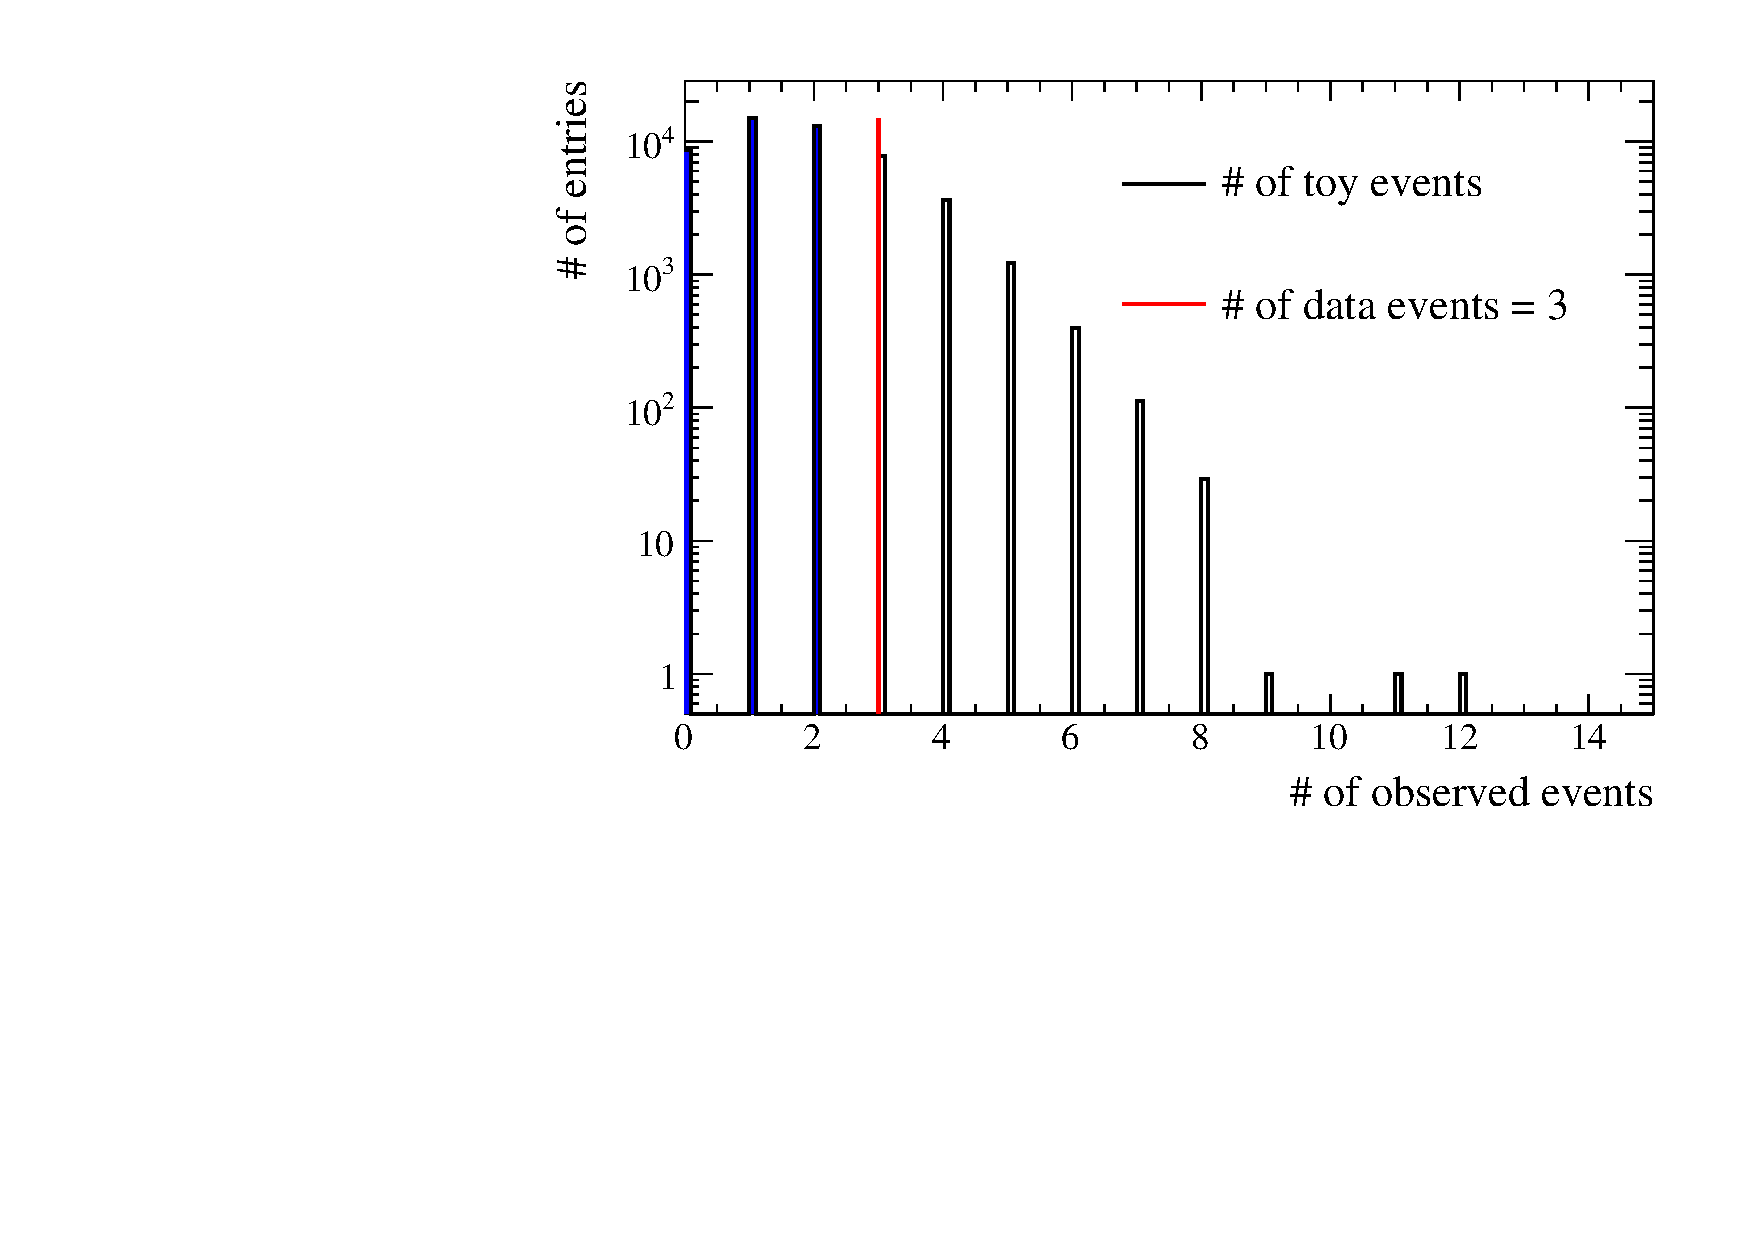
\includegraphics[width=0.9\textwidth]{./nuebar_plots/results/pvalue_rateonly_50ktoys}
%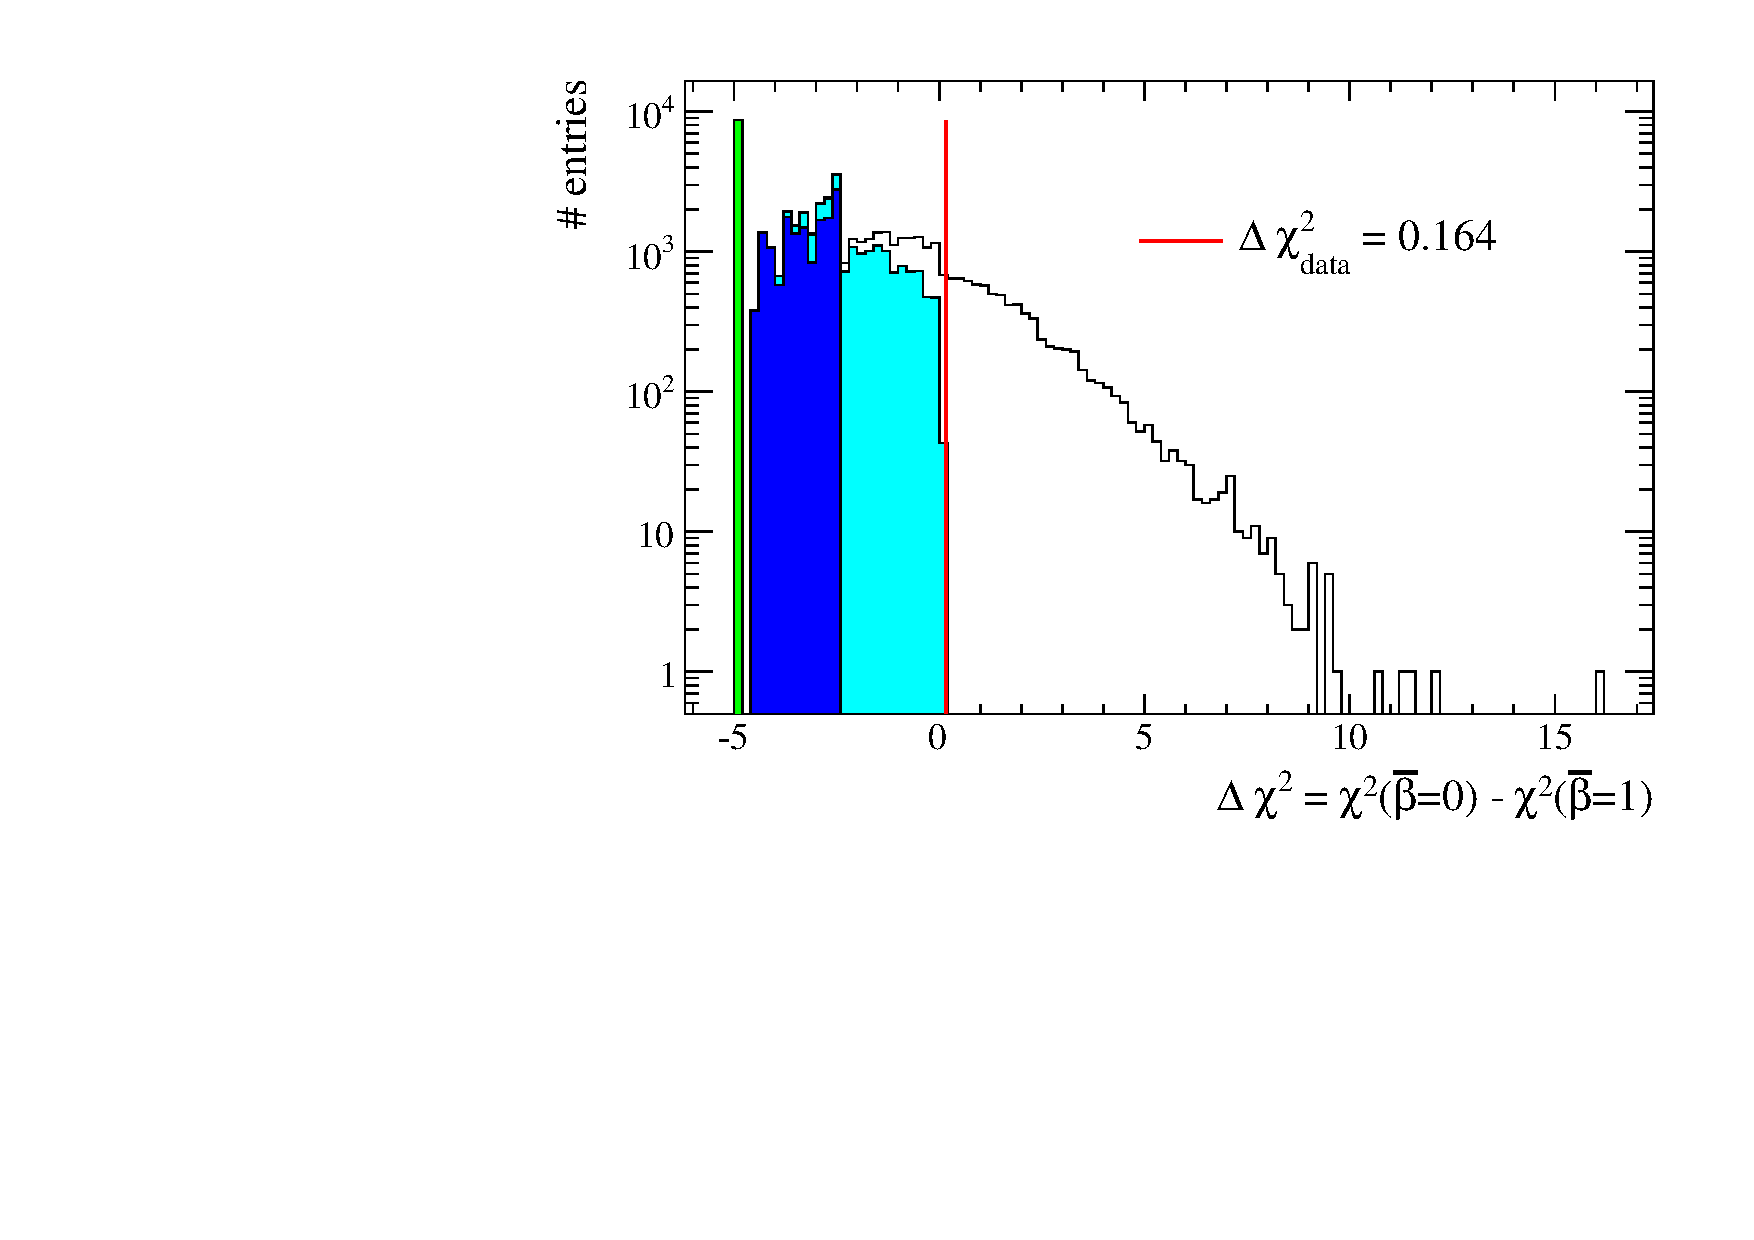
\includegraphics[width=0.9\textwidth]{./nuebar_plots/results/pvalue_rateshape_50ktoys}
\begin{subfigure}[b]{0.49\textwidth}
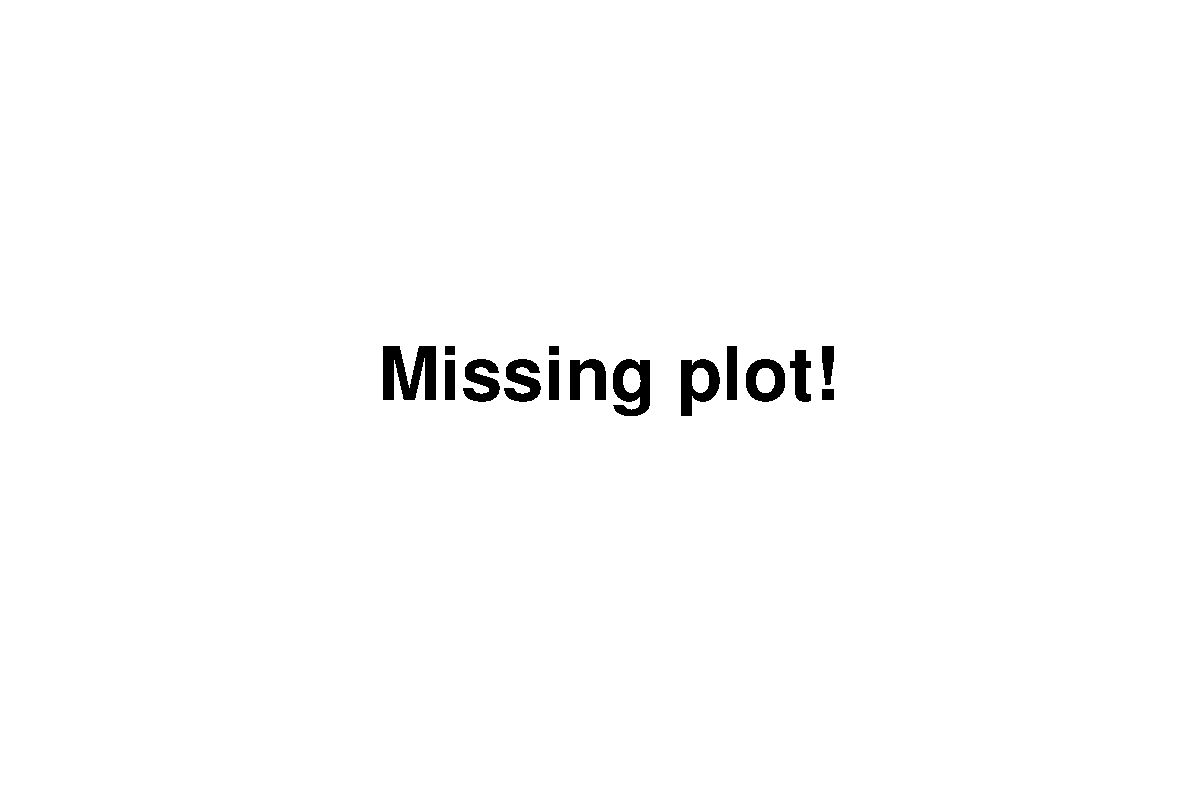
\includegraphics[width=0.9\textwidth]{./images/missing_plot-eps-converted-to.pdf}
\caption{Caption}
\end{subfigure}
\begin{subfigure}[b]{0.49\textwidth}
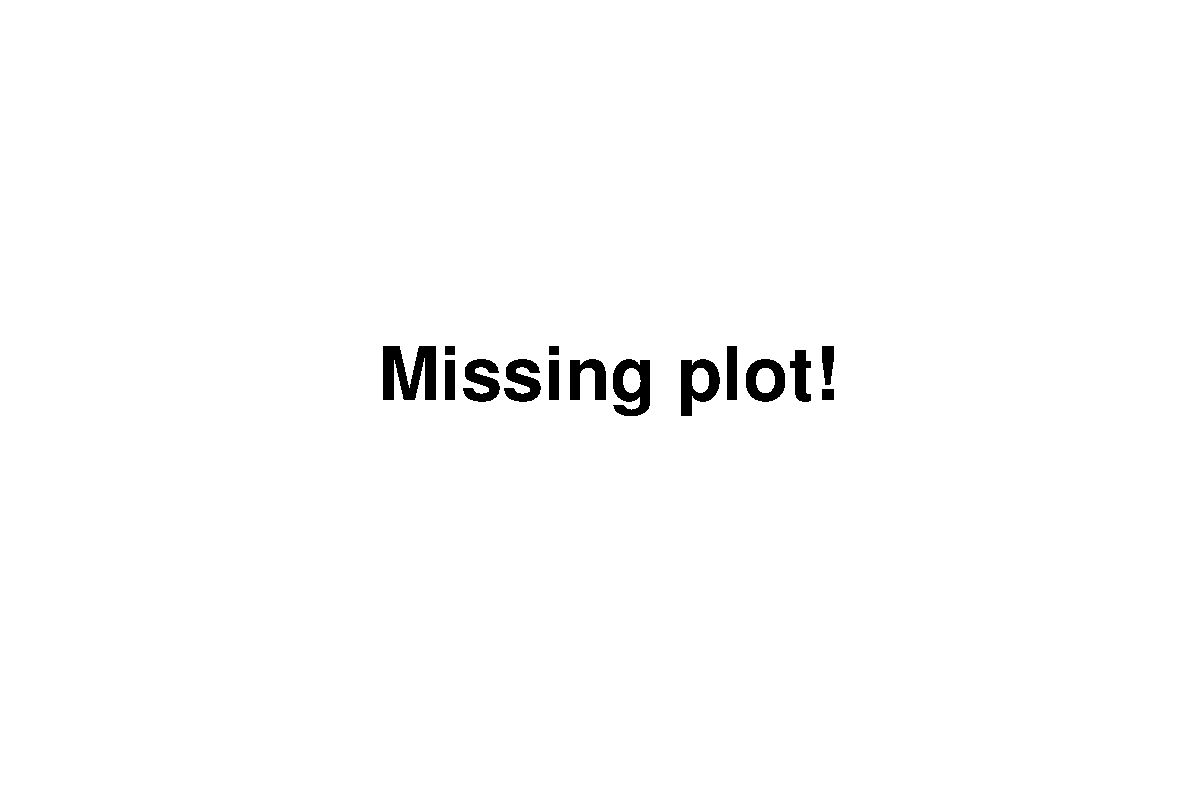
\includegraphics[width=0.9\textwidth]{./images/missing_plot-eps-converted-to.pdf}
\caption{Caption}
\end{subfigure}
\caption {
%{\huge TO UPDATE} 
The distribution of the total number of events from each of the \NumToysLarge toy experiments. 
The red line corresponds to the total number of events (left) and $\Delta \chi^2$ (right) given by the Run 5+6 dataset. 
Data correspond to Run 1-6 statistic. %\TotalPot POT.
The distribution of the test statistics are obtained by performing 50k toys. 
%\FakePotLow POT (left) and \FakePotHigh (right).
}
\label{fig:pvalue_rateonly_data}
\end{figure}


%...........................................................
%
% Table summarizing p-value for different test statistics
%
\begin{table}[htb]
\centering
\begin{tabular}{| c | c | c | c | c | c |}
\hline
Observed num. of events 		& p-value (rate-only)	 	& $\chi^2 (\beta=0)$ 		& $\chi^2 (\beta=1)$	 	& $\Delta \chi^2$ 	& p-value (rate+shape)  	\\
\hline
X				 		& XXX 		 		& XXX				& XXX				& XXX		 	& XXX			  	\\

\hline
\end{tabular}
\caption{
%{\huge TO UPDATE} 
Summary of observed number of events, $\chi^2$ for $\beta=0$ and $\beta=1$, $\Delta \chi^2$, rate-only and rate+shape p-values from the combined Run 5+6 dataset.
The quoted $\chi^2$ values were computed from \cref{eq:loglikemarg},
while $\Delta \chi^2$ from \cref{eq:deltachisq_rateshape} in \cref{sec:oscfit_method}.
using the reconstructed energy binning scheme given in \cref{sec:mc_templates:template_binning}.
The p-values are obtained performing \NumToysLarge toys with $\beta=0$ in order to get the distribution of the test statistic.
}
\label{tab:results}
\end{table}


%...........................................................

% Discussion about the p-value
%

The distribution of the expected test statistics, compared with the one obtained from the Run5-6 dataset, is shown in \cref{fig:pvalue_rateonly_data}.


%...........................................................
%
% Delta Chisq and # of events distributions with data overlapped signal and bkg
%

In \cref{fig:pvalue_rateonly_sigbkg} and \cref{fig:pvalue_rateshape_sigbkg}
the distributions of the test statistic, for rate-only and rate+shape analyses, are shown and compared with the data.
It is already clear that the current dataset is compatible with both $\beta=0$ and $\beta=1$, since the 
significance for both cases is not large enough.

\begin{figure}
\center
%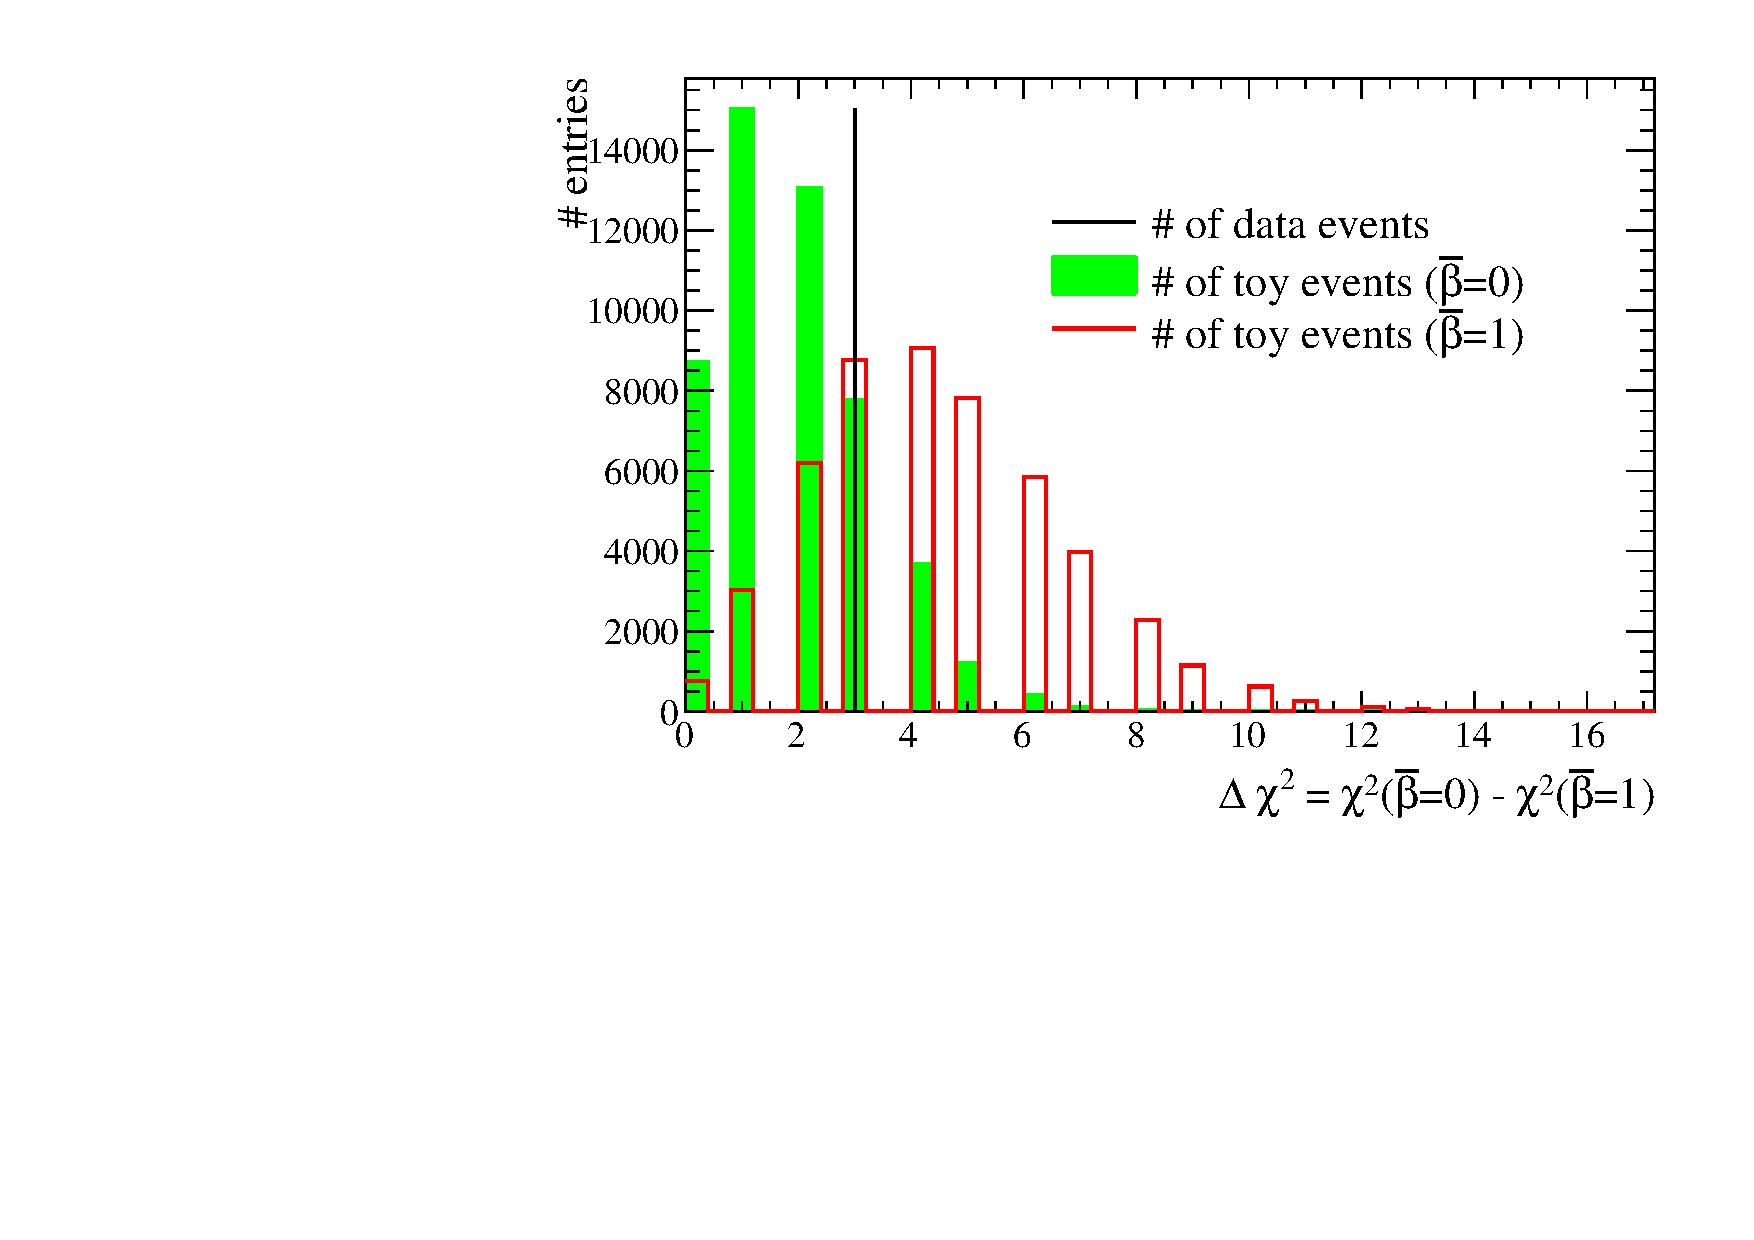
\includegraphics[width=0.9\textwidth]{./nuebar_plots/results/pvalue_rateonly_sigbkg_50ktoys.pdf}
%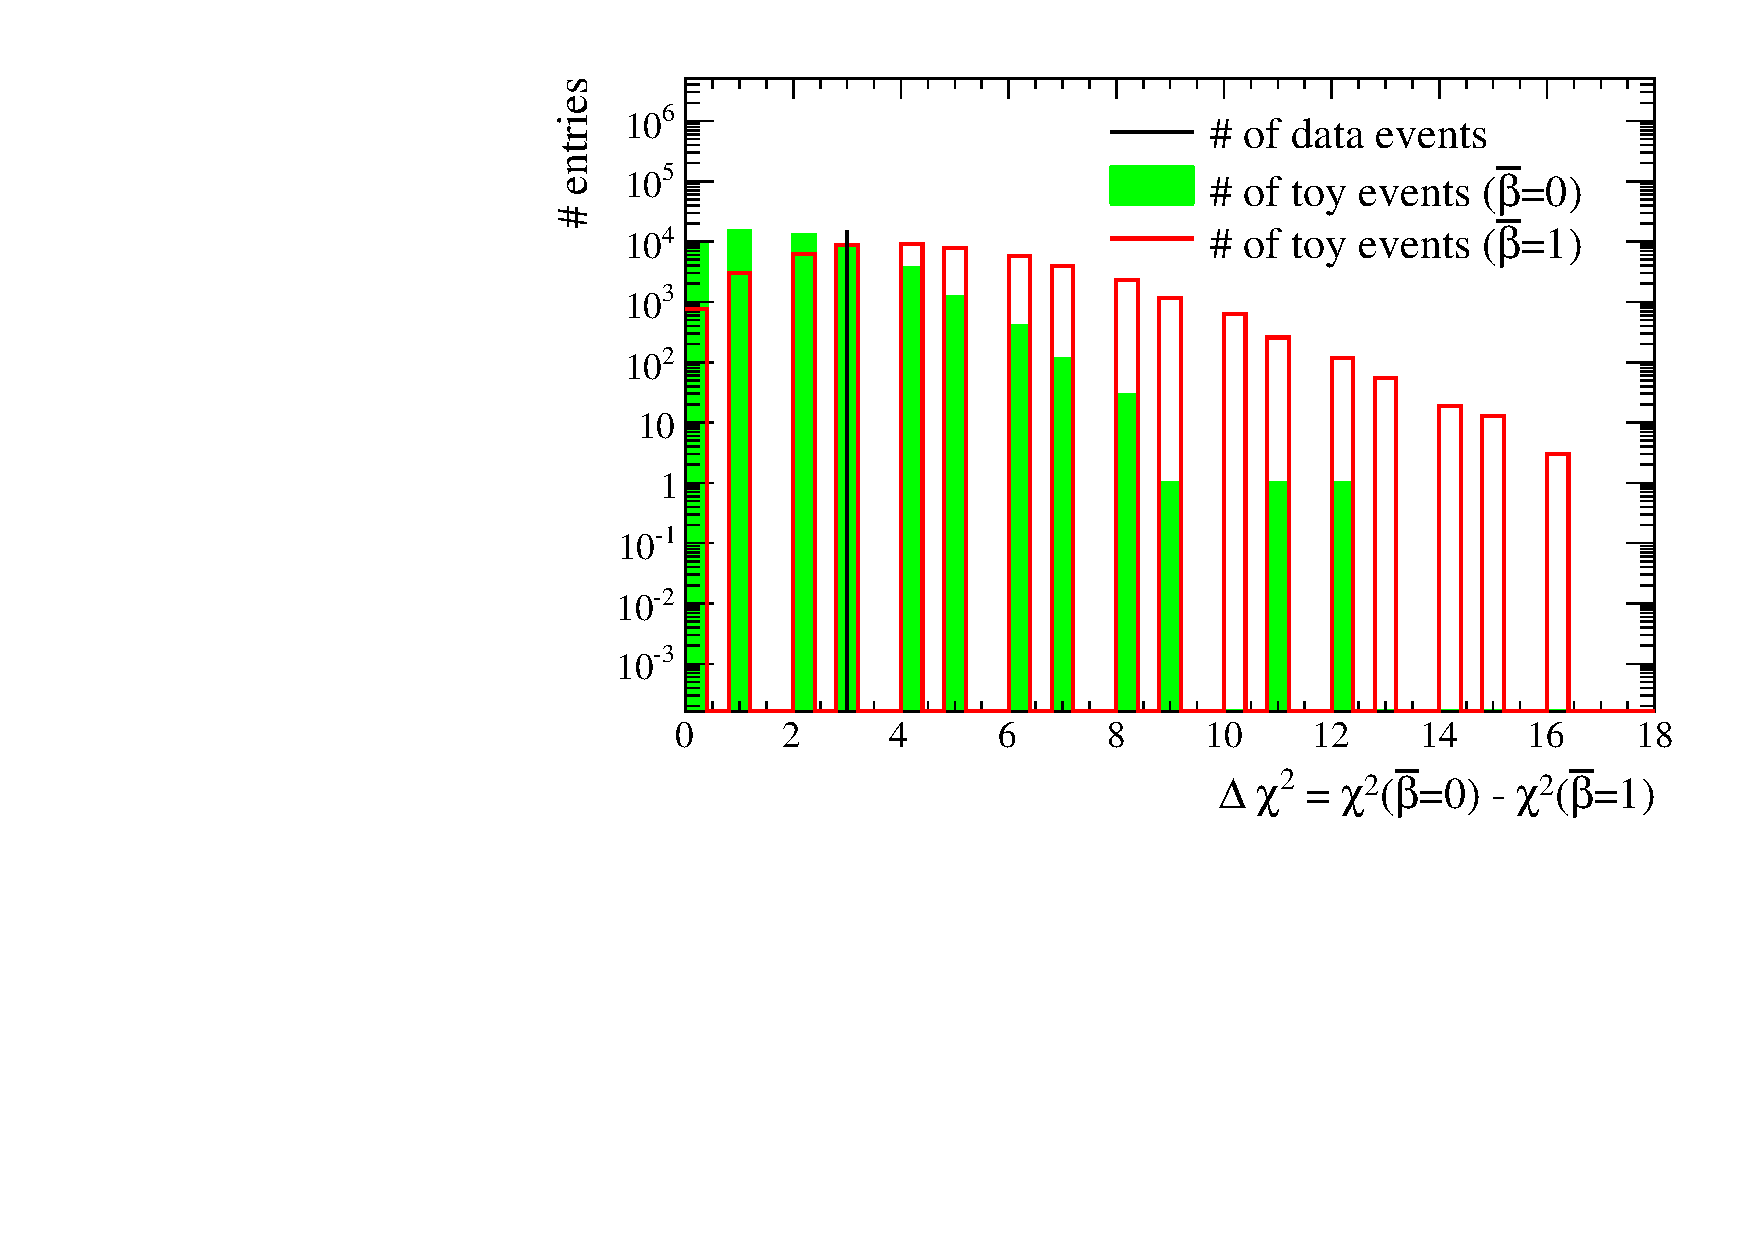
\includegraphics[width=0.9\textwidth]{./nuebar_plots/results/pvalue_rateonly_sigbkg_50ktoys_log_zoom.pdf}
\begin{subfigure}[b]{0.49\textwidth}
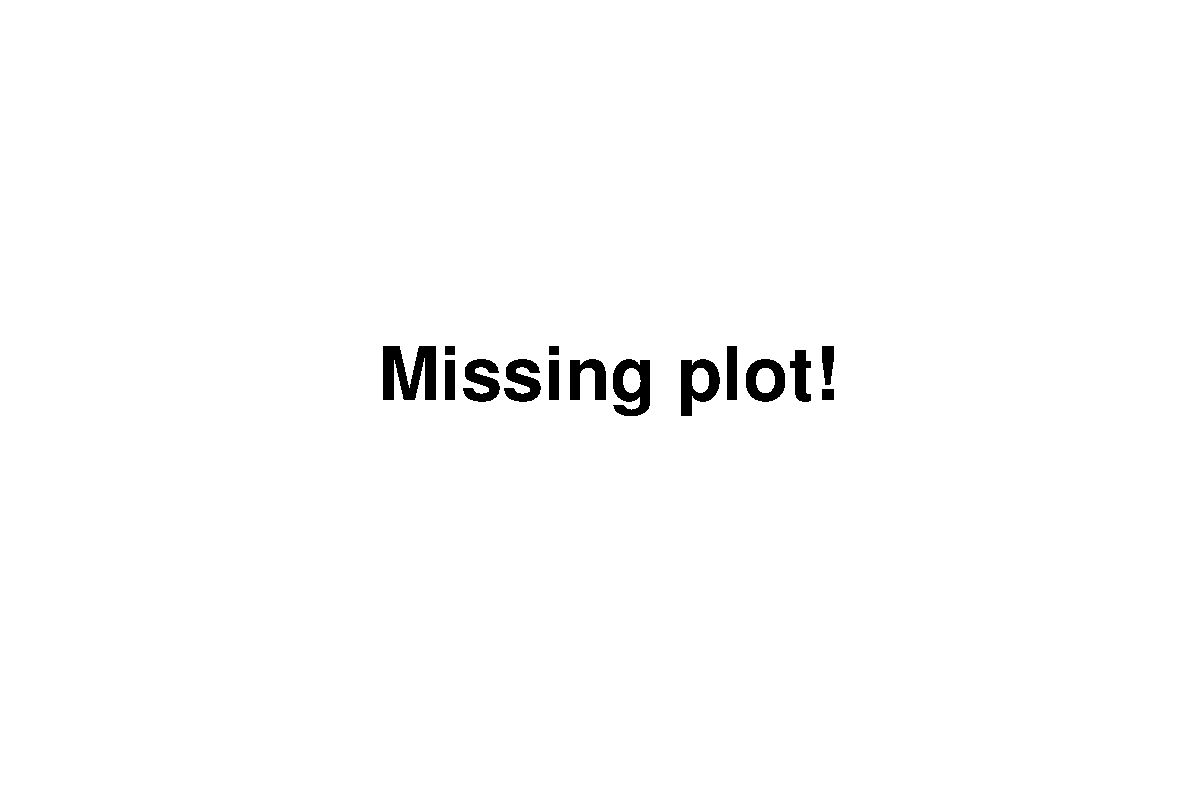
\includegraphics[width=0.9\textwidth]{./images/missing_plot-eps-converted-to.pdf}
\caption{Caption}
\end{subfigure}
\begin{subfigure}[b]{0.49\textwidth}
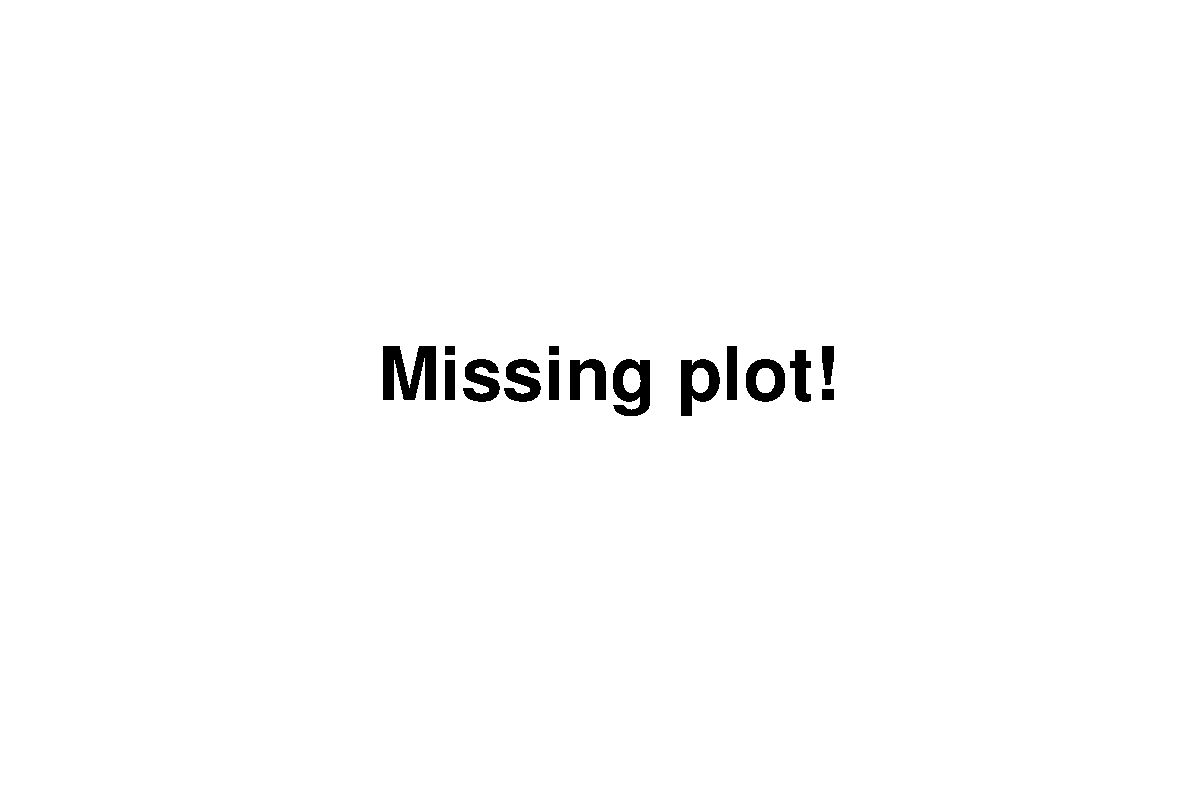
\includegraphics[width=0.9\textwidth]{./images/missing_plot-eps-converted-to.pdf}
\caption{Caption}
\end{subfigure}
\caption {
%{\huge TO UPDATE} 
The distribution of the total number of events from each of the \NumToysLarge toy experiments is
shown for both $\beta=0$ (green) and $\beta=1$ (red).
The black line corresponds to the total number of events observed in the Run 5+6 dataset. 
Data correspond to Run 1-6 statistic. %\TotalPot POT.
Both linear (left) and logarithmic (right) scales are shown.
}
\label{fig:pvalue_rateonly_sigbkg}
\end{figure}

\begin{figure}
\center
%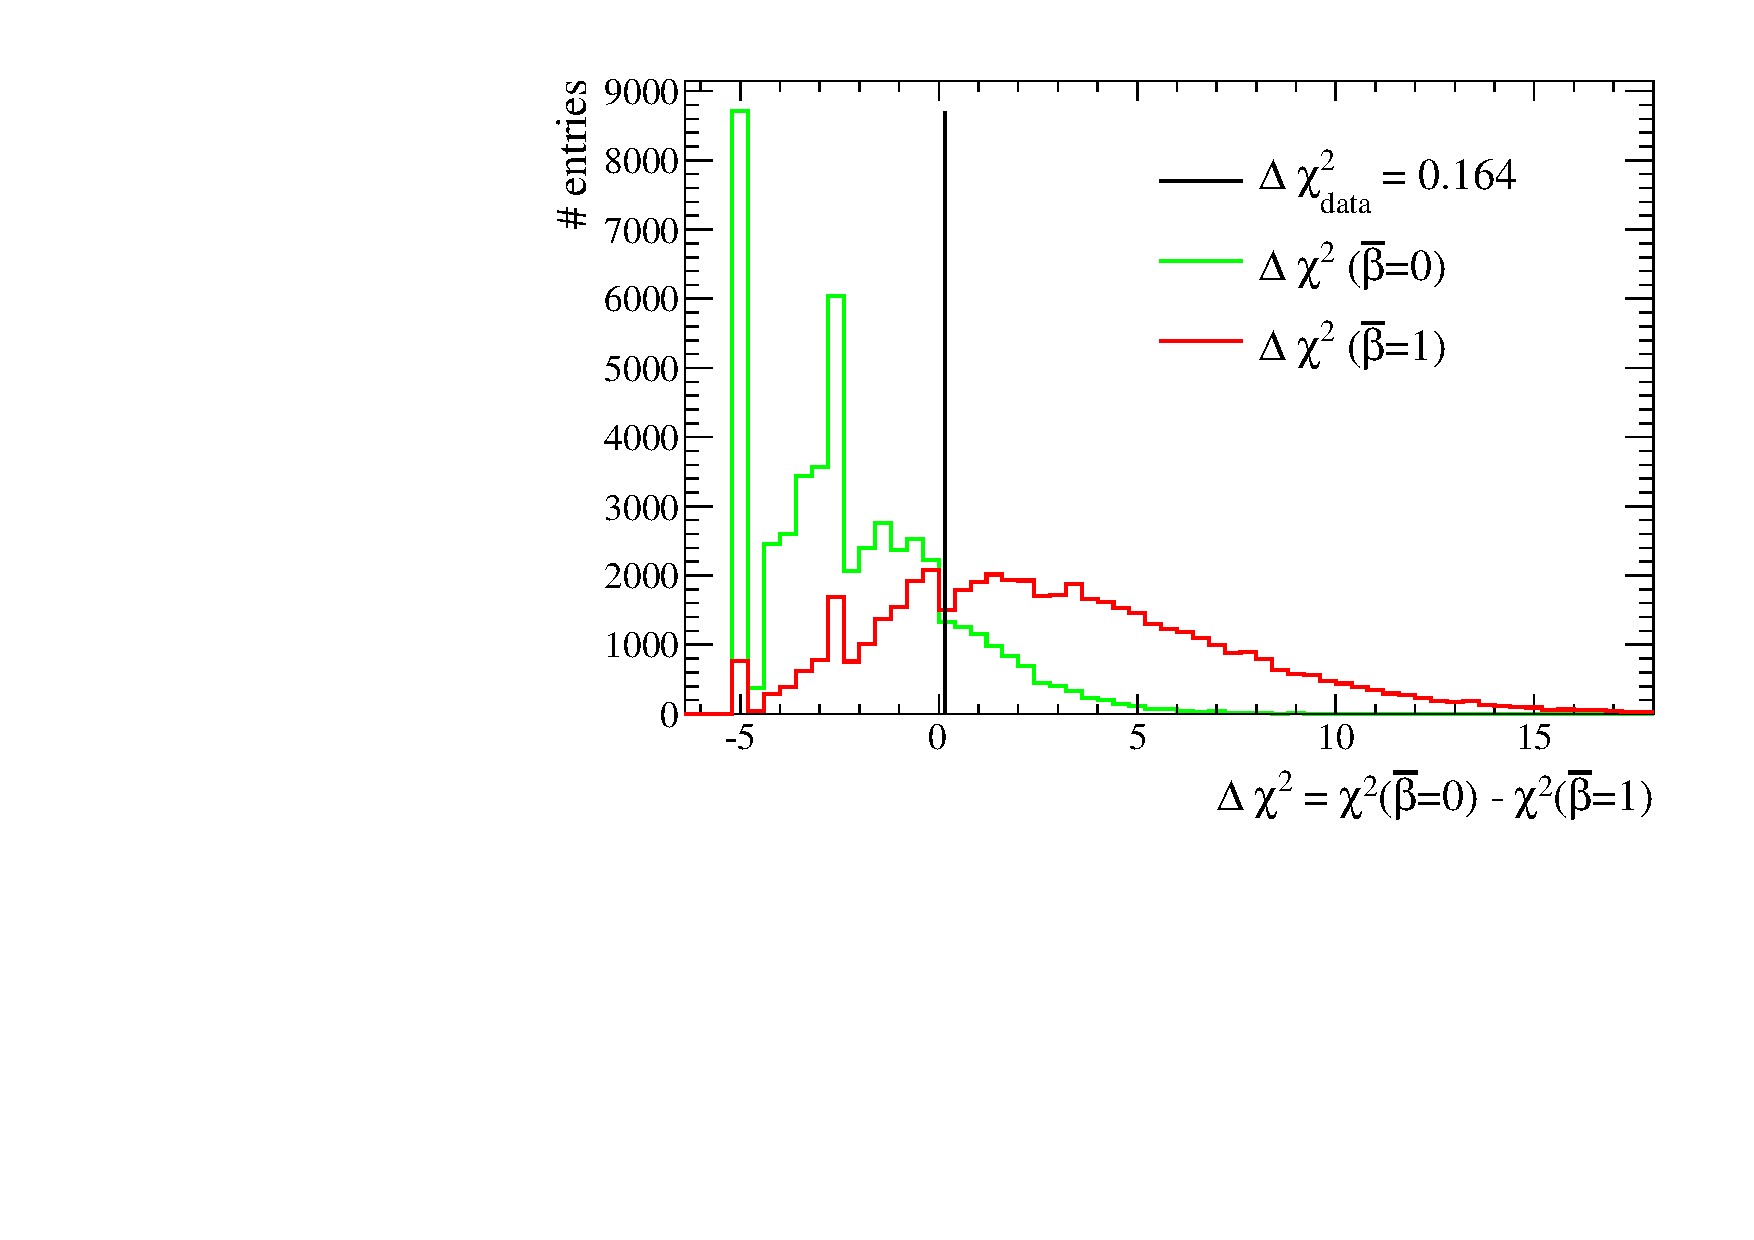
\includegraphics[width=0.9\textwidth]{./nuebar_plots/results/pvalue_rateshape_sigbkg_50ktoys.pdf}
%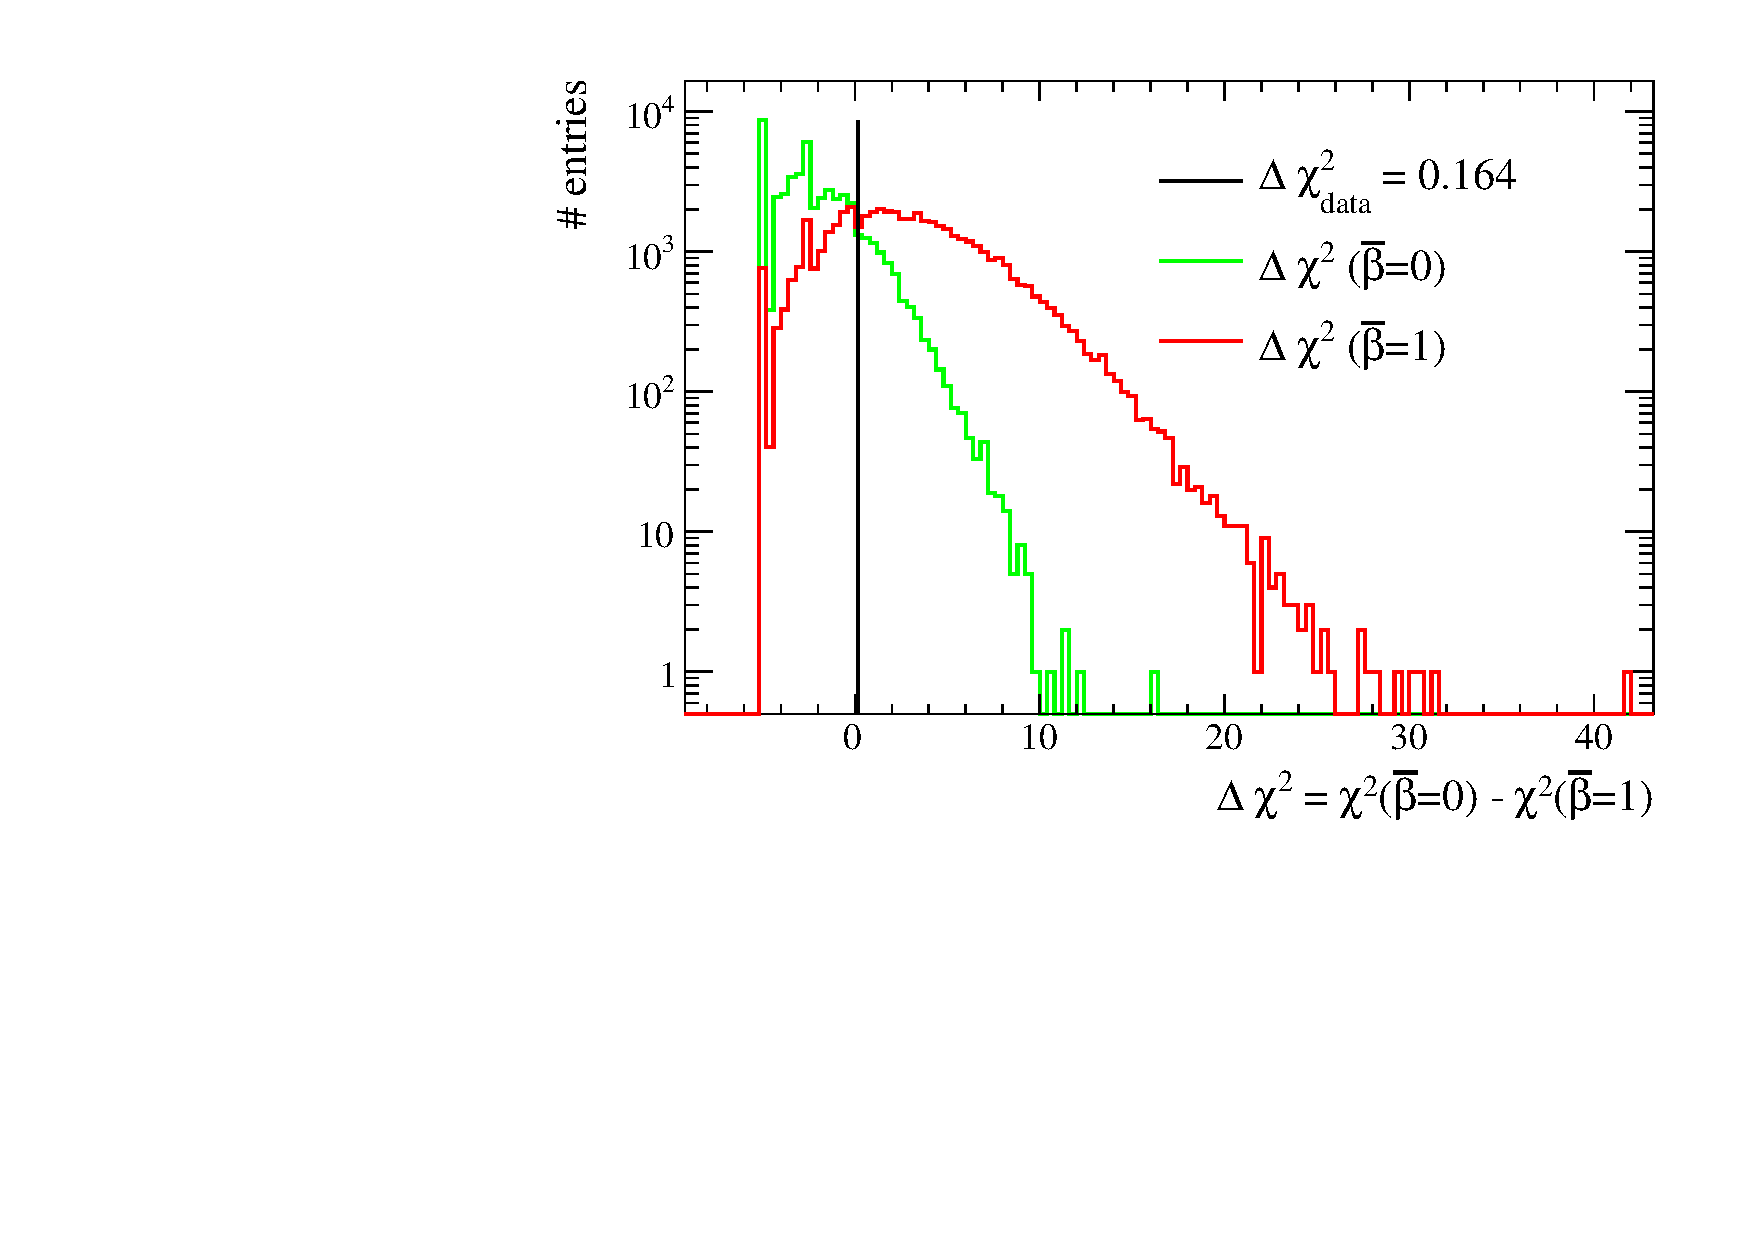
\includegraphics[width=0.9\textwidth]{./nuebar_plots/results/pvalue_rateshape_sigbkg_50ktoys_log.pdf}
\begin{subfigure}[b]{0.49\textwidth}
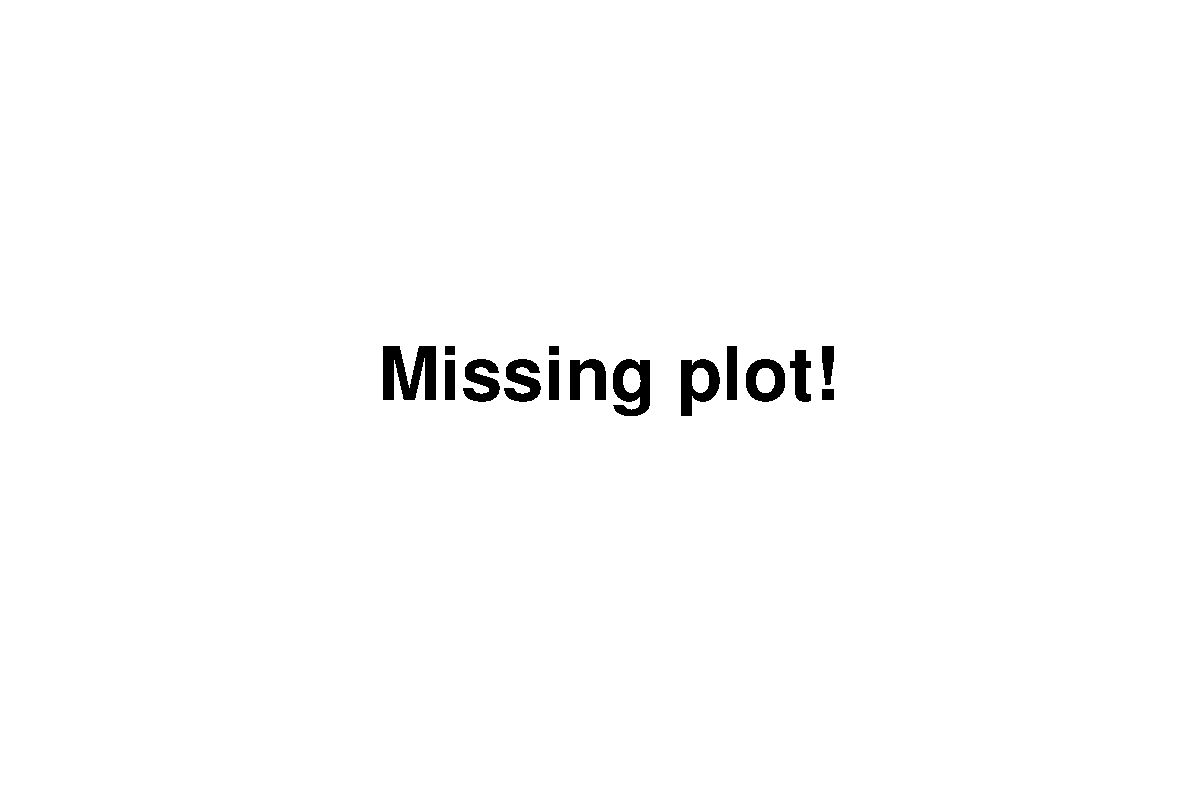
\includegraphics[width=0.9\textwidth]{./images/missing_plot-eps-converted-to.pdf}
\caption{Caption}
\end{subfigure}
\begin{subfigure}[b]{0.49\textwidth}
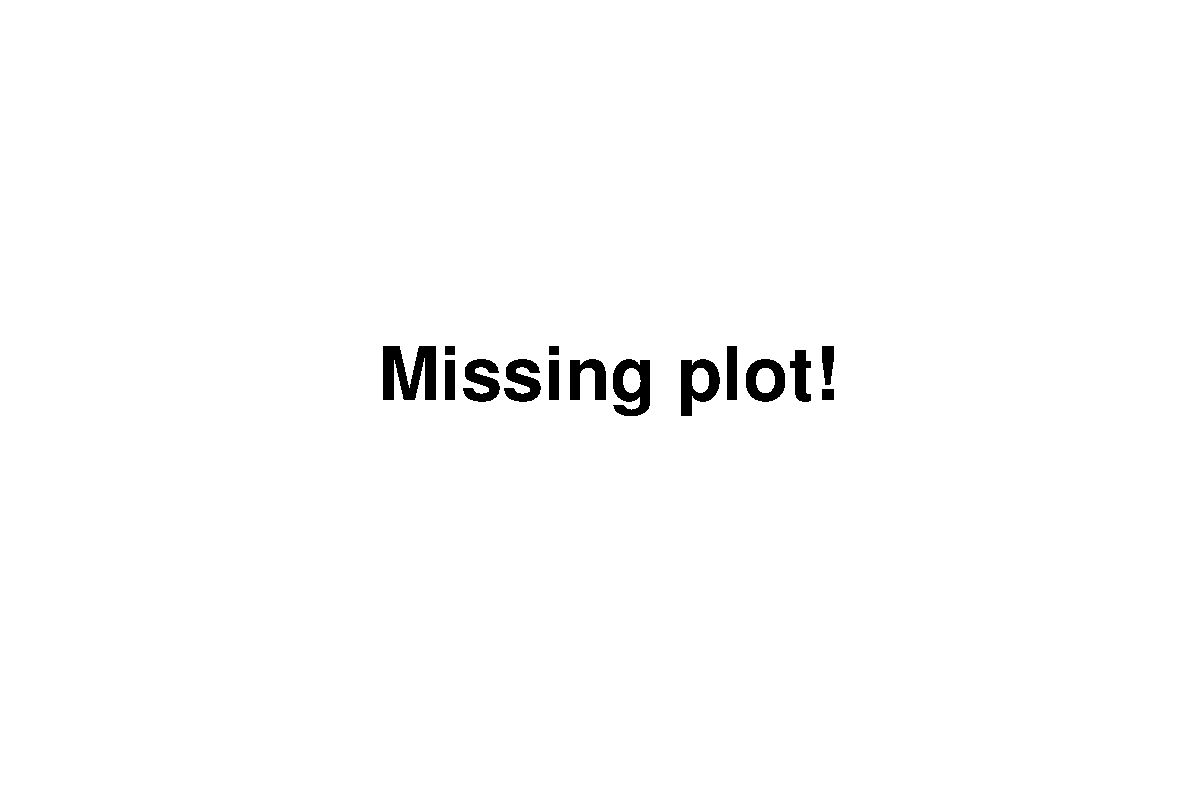
\includegraphics[width=0.9\textwidth]{./images/missing_plot-eps-converted-to.pdf}
\caption{Caption}
\end{subfigure}\caption {
%{\huge TO UPDATE} 
The distribution of the test statistic $\Delta \chi^2$ for each of the \NumToysLarge toy experiments is shown for
both $\beta=0$ (green) and $\beta=1$ (red). 
The black line corresponds to the $\Delta \chi^2$ obtained from the Run 5+6 dataset. 
Data correspond to Run 1-6 statistic. %\TotalPot POT.
Both linear (left) and logarithmic (right) scales are shown.
}
\label{fig:pvalue_rateshape_sigbkg}
\end{figure}

In order to quantify it, the 1-sided p-value given $\bar{\nu}_e$ appearance was calculated as well.
In this case, contrary to the case of null $\bar{\nu}_e$ appearance hypothesis, the 1-sided p-value
is computed on the left tail of the expected distribution of the test statistic, where the 
observed value of $\Delta \chi^2$ is placed.
As shown in \cref{tab:results_bkg} the p-value given $\bar{\nu}_e$ appearance is slightly larger than 
the background only hypothesis. The fit slightly prefers the hypothesis of $\bar{\nu}_e$ appearance,
though the significance is not large enough to claim any possible hint yet.
% of $\bar{\nu}_e$ appearance.

%...........................................................
%
% Table summarizing p-value for different test statistics
%
\begin{table}[htb]
\centering
\begin{tabular}{| c | c | c | c | c | c |}
\hline
hypothesis		 		& p-value (rate-only)	  	& p-value (rate+shape)  	\\
\hline
$\beta=0.5$			  	& 0.246 			 	& XXX			  	\\
\hline
$\beta=1$			 		& 0.089 			 	& XXX			  	\\
\hline
$\beta=1.5$				& 0.123 			 	& XXX			  	\\
\hline
$\beta=2$			 		& 0.026 			 	& XXX			  	\\
\hline
$\beta=2.5$		 		& 0.010 			 	& XXX			  	\\

\hline
\end{tabular}
\caption{
%{\huge TO UPDATE} 
Summary of 1-sided rate-only and rate+shape p-values from the combined Run 5+6 dataset.
The 1-sided p-values are obtained performing 50k toys with $\beta=0$ for background only hypothesis
and $\beta=1$ for $\bar{\nu}_e$ appearance hypothesis, in order to get the distribution of the test statistic.
In the first case the p-value given null $\bar{\nu}_e$ appearance is obtained on the right tail of the expected distribution,
while for $\beta=1$ the 1-sided p-value is obtained on the left tail of the expected distribution.
}
\label{tab:results_bkg}
\end{table}





\clearpage
